% ----------------------------------------------------------------
% Thesis - Main document
% ----------------------------------------------------------------

\documentclass{thesisclass}
% as defined in thesisclass.cls


%% ------------------------- --------
%% | Information about the thesis  |
%% ---------------------------------

\newcommand{\myname}{Muti Ur Rehman}
\newcommand{\mytitle}{Panoptic Segmentation for Urban Scenarios}

\newcommand{\reviewerone}{Prof. Dr.-Ing. Christoph Stiller}
\newcommand{\advisorone}{Frank Bieder, M.Sc.}
\newcommand{\reviewertwo}{Prof. Dr.-Ing. Michael Heizmann}
\newcommand{\advisortwo}{Hannes Weinreuter, M.Sc.}

\newcommand{\timeandplace}{Karlsruhe, September 2020}

\newcommand{\frontmatterhint}{Draft! / Vorl\"aufige Fassung!}

\definecolor{c1}{HTML}{9ACFC6}
\definecolor{c2}{HTML}{DABBD6}
\definecolor{c3}{HTML}{CBDCB9}
\definecolor{c4}{HTML}{9AC3E1}
\definecolor{c5}{HTML}{DEBBA5}
\definecolor{c6}{HTML}{C4DDE5}
\newcommand*{\xMin}{0}%
\newcommand*{\xMax}{6}%
\newcommand*{\yMin}{0}%
\newcommand*{\yMax}{4}%

\newcommand*{\xMinR}{9.5}%
\newcommand*{\xMaxR}{12.5}%
\newcommand*{\yMinR}{1}%
\newcommand*{\yMaxR}{3}%


%% -------------------------------
%% |  Information for PDF file   |
%% -------------------------------
\hypersetup{
 pdfauthor={\myname},
 pdftitle={\mytitle},
 pdfsubject={Thesis},
 pdfkeywords={}
}
\usepackage[english]{babel}  	% English
%\usepackage[ngerman]{babel}  	% German


%% -------------------------------
%% |    My packages /commands    |
%% -------------------------------
% track changes
    %\usepackage{changes} 		% highlight changes
	\usepackage[final]{changes}	% don't highlight changes

% tables
	\usepackage{array,multirow,graphicx}

% pseudocode
	\usepackage[ruled,vlined]{algorithm2e}

% for forcing positions of tables, figures, ...
	\usepackage{float}

% units
	\usepackage{siunitx}
	\usepackage{dcolumn}
	
% Additional
	\usepackage[numbers]{natbib}
	\usepackage{subfigure}
	\usepackage{pgfplots}
    \usepackage{amsmath}
    \usepackage{neuralnetwork}
    \usepackage{ifthen}
    \usepackage{tikz}
    \usepackage{amssymb}
    \usepackage{bm}
    \usetikzlibrary{arrows.meta}
    \usetikzlibrary{decorations.pathreplacing}
    \usetikzlibrary{matrix, positioning}
    \usepackage{pdfpages}
    %\usepackage{natbib}
    \usepackage{natbib}
    \usepackage{rotating}
    \usepackage{array}
    \usepackage{booktabs}


%% --------------------------------
%% |      glossaries               |
%% --------------------------------
\newif\ifuseglossaries			% as the glossaries package sometimes causes problems, you can switch if of
								% if switching of, remember to remove all \gls{}/... statements
								
\useglossariestrue				% use glossaries (acronyms and online references)
%\useglossariesfalse			% don't use glossaries

\ifuseglossaries
	\usepackage[acronym,xindy,toc,nomain,nonumberlist,nopostdot,notranslate]{glossaries}%

	\newglossary[onlineref]{onlineref}{onli}{onlo}{Online References}
	
	\newglossarystyle{mylong}{%
  		\setglossarystyle{long}%
  		\renewcommand*{\glsnamefont}[1]{\textbf{##1}}%
  	}%
  	
  	\newglossarystyle{mylist}{%
  		\setglossarystyle{list}%
  		\renewcommand*{\glsnamefont}[1]{\textrm{\textmd{##1}}}%
  	}%
  	
  	\makeglossaries
  	
	% ordinary acronyms
	\newacronym{ma}{MA}{My Acronym}
	\newacronym{iou}{IOU}{Intersection over Union}
	\newacronym{sq}{SQ}{Segmentation Quality}	
	\newacronym{rq}{RQ}{Recognition Quality}
	\newacronym{pq}{PQ}{Panoptic Quality}
	\newacronym{fcn}{FCN}{Fully Convolutional Network}
	\newacronym{cnns}{CNNs}{Convolutional Neural Networks}
	\newacronym{mlp}{MLP}{Multi-Layer Perceptron}
	\newacronym{anns}{ANNs}{Artificial Neural Networks}
	\newacronym{sgd}{SGD}{Stochastic Gradient Descent}
	\newacronym{tp}{TP}{True Positive}
	\newacronym{fp}{FP}{False Positive}
	\newacronym{fn}{FN}{False Negative}
	\newacronym{nms}{NMS}{Non-Maxima Suppression}
	\newacronym{gpu}{GPU}{Graphics Processing Unit}
	\newacronym{pc}{PC}{Parsing Covering}
	\newacronym{gd}{GD}{Gradient Descent}
	\newacronym{aspp}{ASPP}{Atrous Spatial Pyramid Pooling Module}
	% usage: \gls{} \glspl{} or \acrshort{}
	
	% online references
	\newglossaryentry{online_reference}{
		type=onlineref, 
		name={[01]}, 
		description={\hspace{1.5mm}My Online Reference\newline 
			\href{http://www.mrt.kit.edu/}{http://www.mrt.kit.edu/}\newline 
			retrieved 2016-04-28 }}
\else
\fi


%% ---------------------------------
%% | ToDo Marker - only for draft! |
%% ---------------------------------
% Remove this section for final version!
\setlength{\marginparwidth}{20mm}

\newcommand{\margtodo}
{\marginpar{\textbf{\textcolor{blue}{ToDo}}}{}}

\newcommand{\todoo}[1]
{{\textbf{\textcolor{blue}{(\margtodo{}1)}}}{}}

\newcommand{\margmajortodo}
{\marginpar{\textbf{\textcolor{red}{ToDo}}}{}}

\newcommand{\majortodo}[1]
{{\textbf{\textcolor{red}{(\margmajortodo{}#1)}}}{}}


\newcolumntype{P}[2]{%
  >{\begin{turn}{#1}\begin{minipage}{#2}\small\raggedright\hspace{0pt}}l%
  <{\end{minipage}\end{turn}}%
}

%% --------------------------------
%% | Draft Marker - only for draft! |
%% --------------------------------
% Remove this section for final version!
%\usepackage{draftwatermark}
%\SetWatermarkText{\hspace{10pt}-draft-}
%\SetWatermarkScale{2.3}
%\SetWatermarkColor[gray]{0.95}


%% --------------------------------
%% | Old Marker - only for draft! |
%% --------------------------------
% Remove this section for final version!
\newenvironment{deprecated}
{\begin{color}{gray}}
{\end{color}}


%% --------------------------------
%% | Settings for word separation |
%% --------------------------------
% Help for separation:
% In german package the following hints are additionally available:
% "- = Additional separation
% "| = Suppress ligation and possible separation (e.g. Schaf"|fell)
% "~ = Hyphenation without separation (e.g. bergauf und "~ab)
% "= = Hyphenation with separation before and after
% "" = Separation without a hyphenation (e.g. und/""oder)

% Describe separation hints here:
\hyphenation{
Wort-tren-nung
% Ma-na-ge-ment  Netz-werk-ele-men-ten
% Netz-werk Netz-werk-re-ser-vie-rung
% Netz-werk-adap-ter Fein-ju-stier-ung
% Da-ten-strom-spe-zi-fi-ka-tion Pa-ket-rumpf
% Kon-troll-in-stanz
}

%%%%%%%%%%%%%%%%%%%%%%%%%%%%%%%%%
%% Here, main documents begins %%
%%%%%%%%%%%%%%%%%%%%%%%%%%%%%%%%%
\begin{document}


\frontmatter

% !TeX root = ../thesis.tex
%% titlepage.tex
%%

% coordinates for the bg shape on the titlepage
\newcommand{\diameter}{20}
\newcommand{\xone}{-15}
\newcommand{\xtwo}{160}
\newcommand{\yone}{15}
\newcommand{\ytwo}{-253}

\begin{titlepage}
% bg shape
\begin{tikzpicture}[overlay]
\draw[color=gray]
 		 (\xone mm, \yone mm)
  -- (\xtwo mm, \yone mm)
 arc (90:0:\diameter pt)
  -- (\xtwo mm + \diameter pt , \ytwo mm)
	-- (\xone mm + \diameter pt , \ytwo mm)
 arc (270:180:\diameter pt)
	-- (\xone mm, \yone mm);
\end{tikzpicture}

	\begin{textblock}{10}[0,0](4,2.5)
		
\includegraphics[width=.3\textwidth]{Graphics/Logos/KITLogo_RGB.pdf}
	\end{textblock}

	\begin{textblock}{10}[0,0](13.5,2.25)
		
\includegraphics[width=.25\textwidth]{Graphics/Logos/mrt.pdf}
	\end{textblock}

	\changefont{phv}{m}{n}	% helvetica
	\vspace*{3.5cm}
	\begin{center}
		\Huge{\mytitle}
		\vspace*{2cm}\\
		\Large{
			\iflanguage{english}{Master's Thesis of}
												  {Masterarbeit\\von}
		}\\
		\vspace*{1cm}
		\huge{\myname}\\
		\vspace*{1cm}
		\Large{
			\iflanguage{english}{Institute of Measurement and Control Systems}
			{Institut f\"ur Mess- und Regelungstechnik}
			\\
      \iflanguage{english}{Karlsruhe Institute of Technology}
			{Karlsruher Institut f\"ur Technologie}
		}
	\end{center}
	\vspace*{1cm}
\Large{
\begin{center}
\begin{tabular}[ht]{l c l}
  \iflanguage{english}{Reviewer}{Gutachter}: & \hfill  & \reviewerone\\
  \iflanguage{english}{Advisor}{Betreuender Mitarbeiter}: & \hfill  & \advisor\\
\end{tabular}
\end{center}
}

\vspace{1cm}

\begin{center}
{\color{red} \frontmatterhint}
\end{center}

\vspace{2cm}
\begin{center}
\large{\timeandplace}
\end{center}


\begin{textblock}{10}[0,0](4,16.8)
\tiny{
	\iflanguage{english}
		{KIT -- The Research University in the Helmholtz Association}
		{KIT -- Die Forschungsuniversit\"at in der Helmholtz-Gemeinschaft}
}
\end{textblock}

\begin{textblock}{10}[0,0](14,16.75)
\large{
	\textbf{www.kit.edu}
}
\end{textblock}

\end{titlepage}

\blankpage
% !TeX root = ../thesis.tex

\chapter*{Declaration / Erkl\"arung}
Ich versichere hiermit wahrheitsgemäß, die Arbeit bis auf die dem Aufgabensteller bereits bekannten Hilfsmittel selbständig angefertigt,
alle benutzten Hilfsmittel vollständig angegeben und alles kenntlich gemacht zu haben, was aus Arbeiten anderer unverändert oder mit Abänderungen entnommen wurde.\\

\vspace{2cm}
\myname \\
Karlsruhe, 29.04.2016\\

\blankpage
% !TeX root = ../thesis.tex

\chapter*{Acknowledgement / Danksagung}

\blankpage
% !TeX root = ../thesis.tex

\chapter*{Abstract}
\addcontentsline{toc}{chapter}{Abstract}

\blindtext



\chapter*{Kurzfassung}
\addcontentsline{toc}{chapter}{Kurzfassung}

\blindtext

\blankpage

\tableofcontents

% Acronyms
\ifuseglossaries
	\newpage
	\thispagestyle{empty}
	\printglossary[type=acronym, style=mylong]
\else
\fi


%% -----------------
%% |   Main part   |
%% -----------------
\mainmatter
\pagenumbering{arabic}
% !TeX root = ../thesis.tex

\chapter{Introduction}
\label{sec:introduction}

%\gls{ma} \gls{online_reference}

This chapter provides a brief introduction to the topic and highlights motivation for the chosen task. It further outlines the research questions contemplated
 during the course of presented work.
%\cite{Stiller2015}


\section{Motivation}

Computer vision has received a lot of attention from research communities specially 
after the advent of deep learning based approaches. Autonomous driving in particular can
leverage such recently developed learning based computer vision methods for perception
of the environment. Semantic segmentation is a task in computer vision where each 
pixel in an image is assigned to a predefined category label (\textit{person, bicycle, car etc}) as shown in \ref{fig:semseg}.
Although, semantic segmentation plays a key role in efficient and holistic semantic 
representation of the scene under observation however highly complex and dynamic situations 
such as urban scenarios which involve multiple traffic participants demand 
an even fine-grained instance-level understanding of the scene. 
Instance segmentation on the other hand deals with delineating each distinct object 
of interest appearing in an image without providing necessary semantic layout information about the scene \ref{fig:instseg}.
\begin{figure}[!ht]
%\centering
    \subfigure[RGB Image]{
        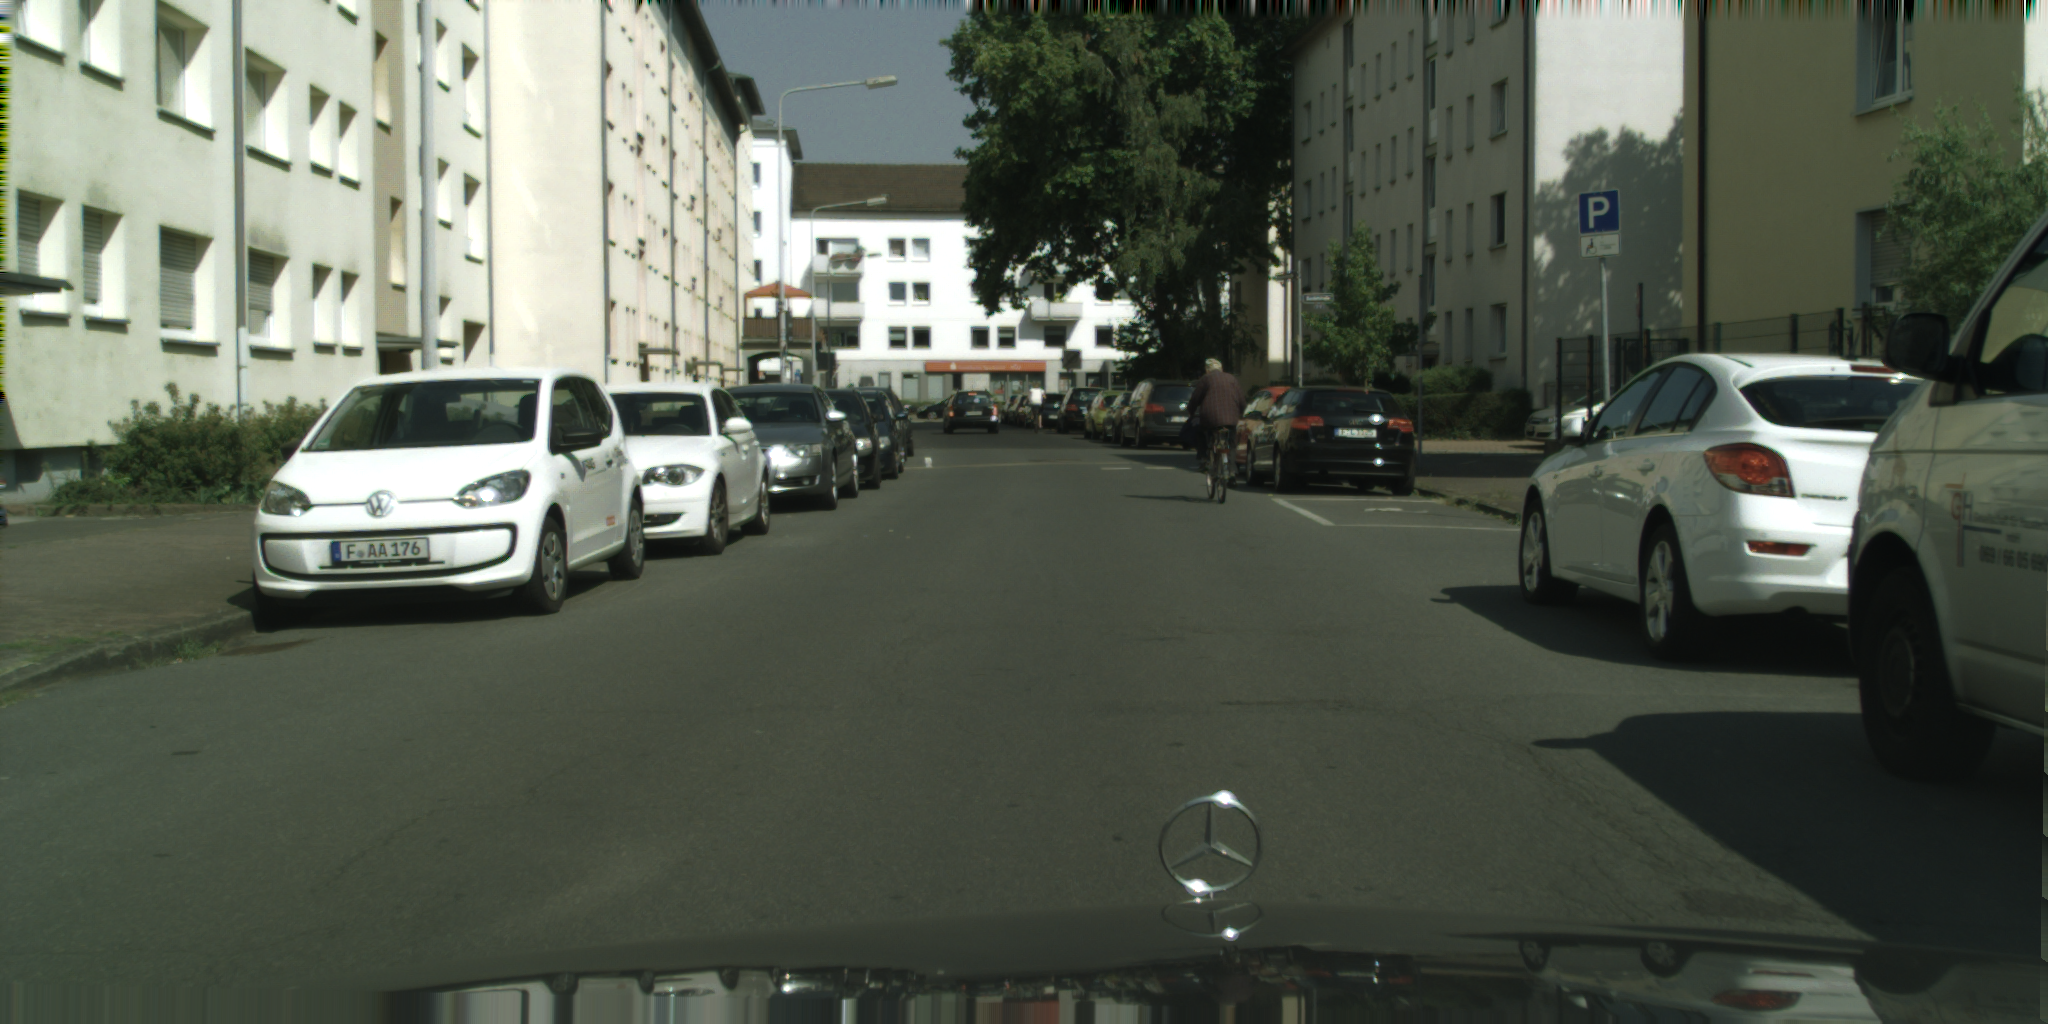
\includegraphics[width = \textwidth / 2 ]{Graphics/Introduction_images/frankfurt_000000_000576_leftImg8bit}
        \label{fig:RGBimage}}
    %\hspace{1pt}
     %add desired spacing between images, e. g. ~, \quad, \qquad, \hfill etc.
     %(or a blank line to force the subfigure onto a new line)
    \subfigure[Semantic Segmentation]{
        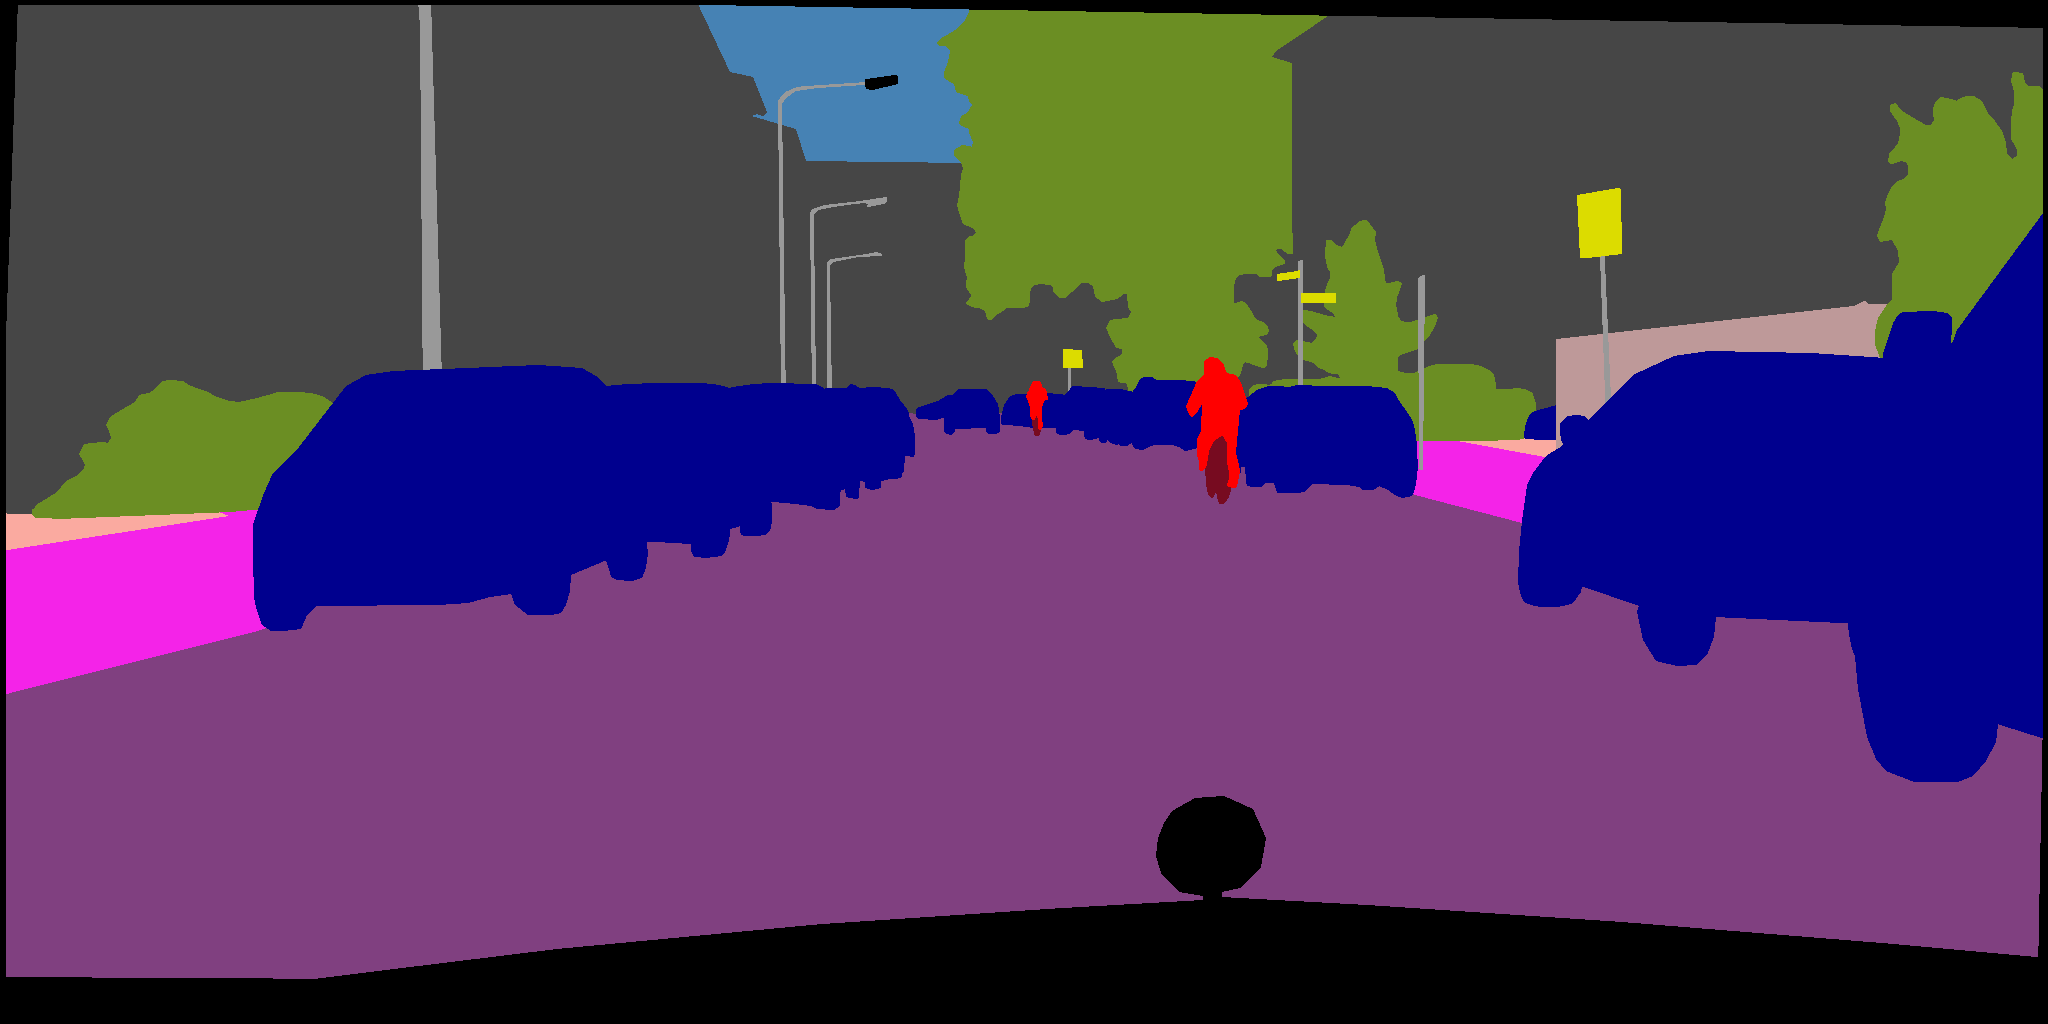
\includegraphics[width = \textwidth / 2 ]{Graphics/Introduction_images/frankfurt_000000_000576_gtFine_color}
        \label{fig:semseg}}
    \subfigure[Instance Segmentation]{
        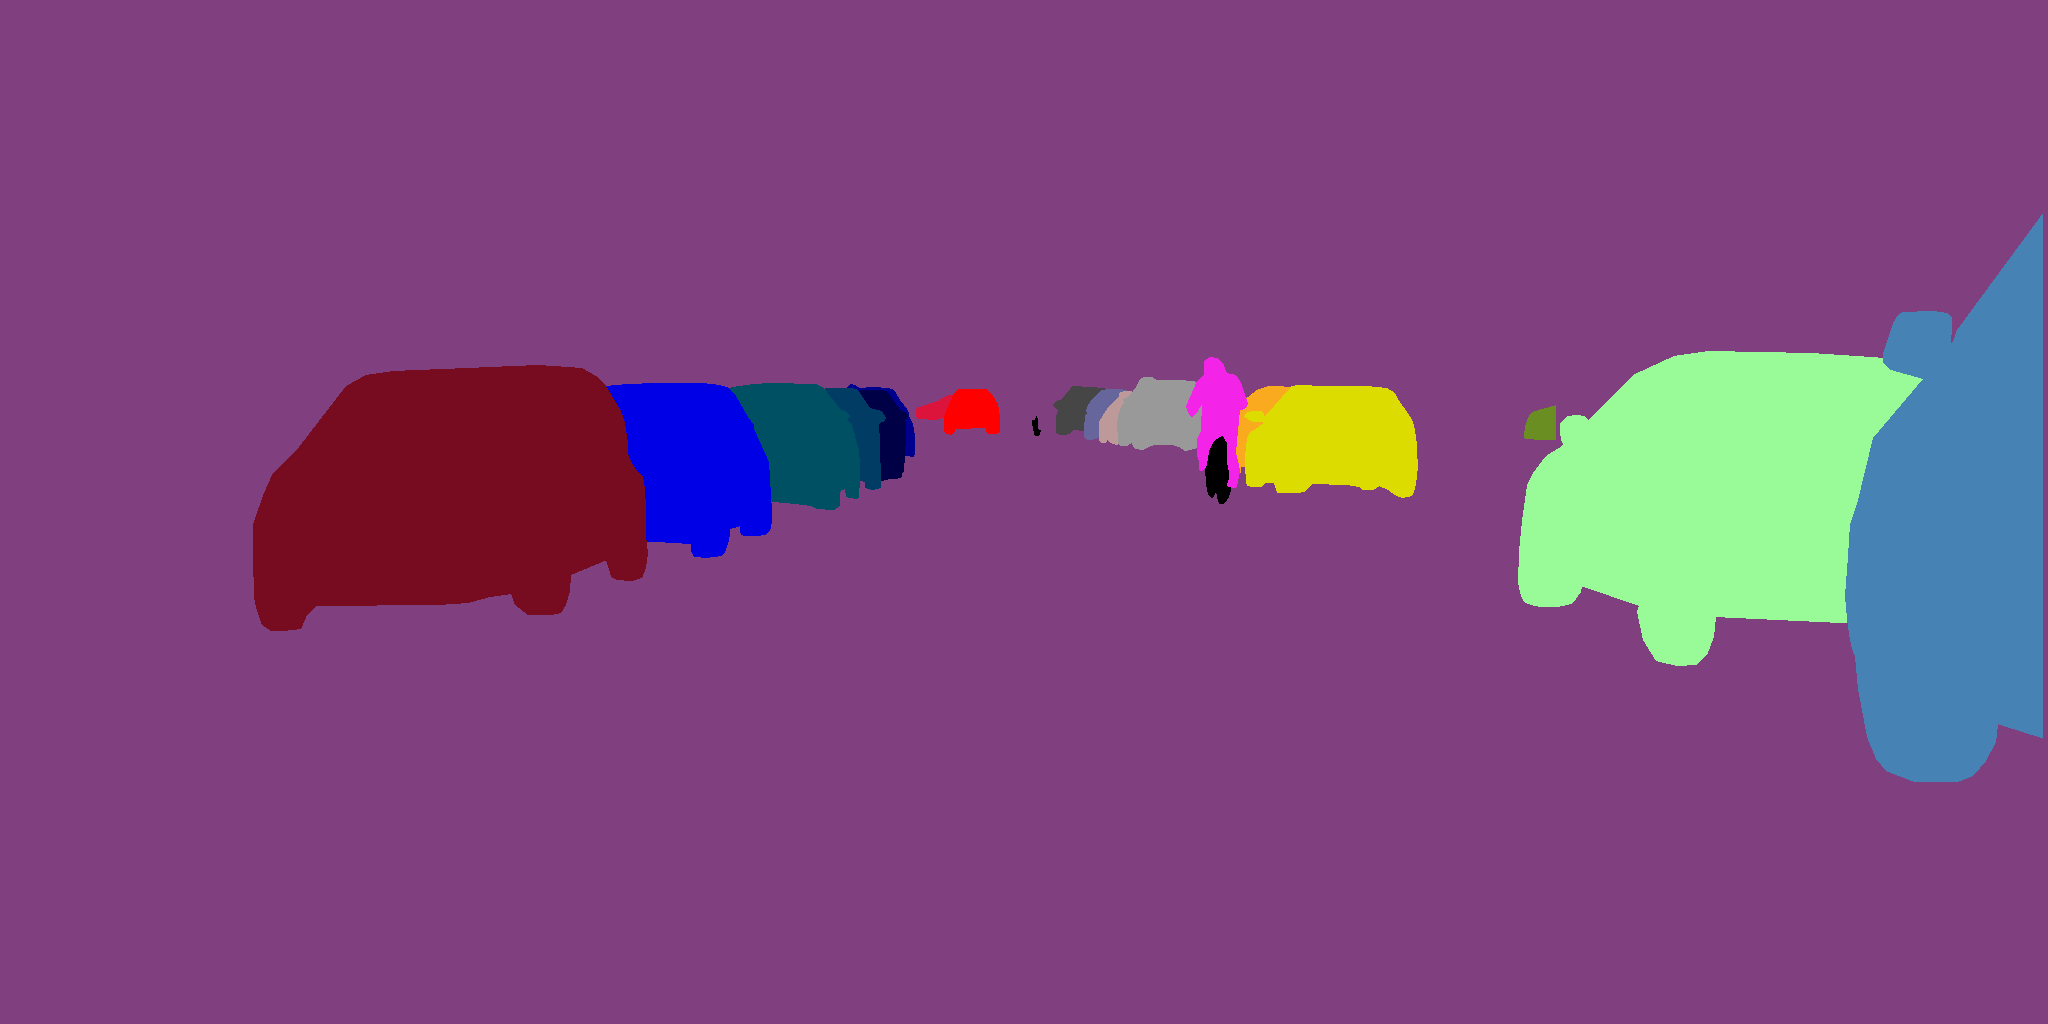
\includegraphics[width = \textwidth / 2 ]{Graphics/Introduction_images/Instance_seg}
        \label{fig:instseg}}
%   \hspace{1pt}
    \subfigure[Panoptic Segmentation]{
        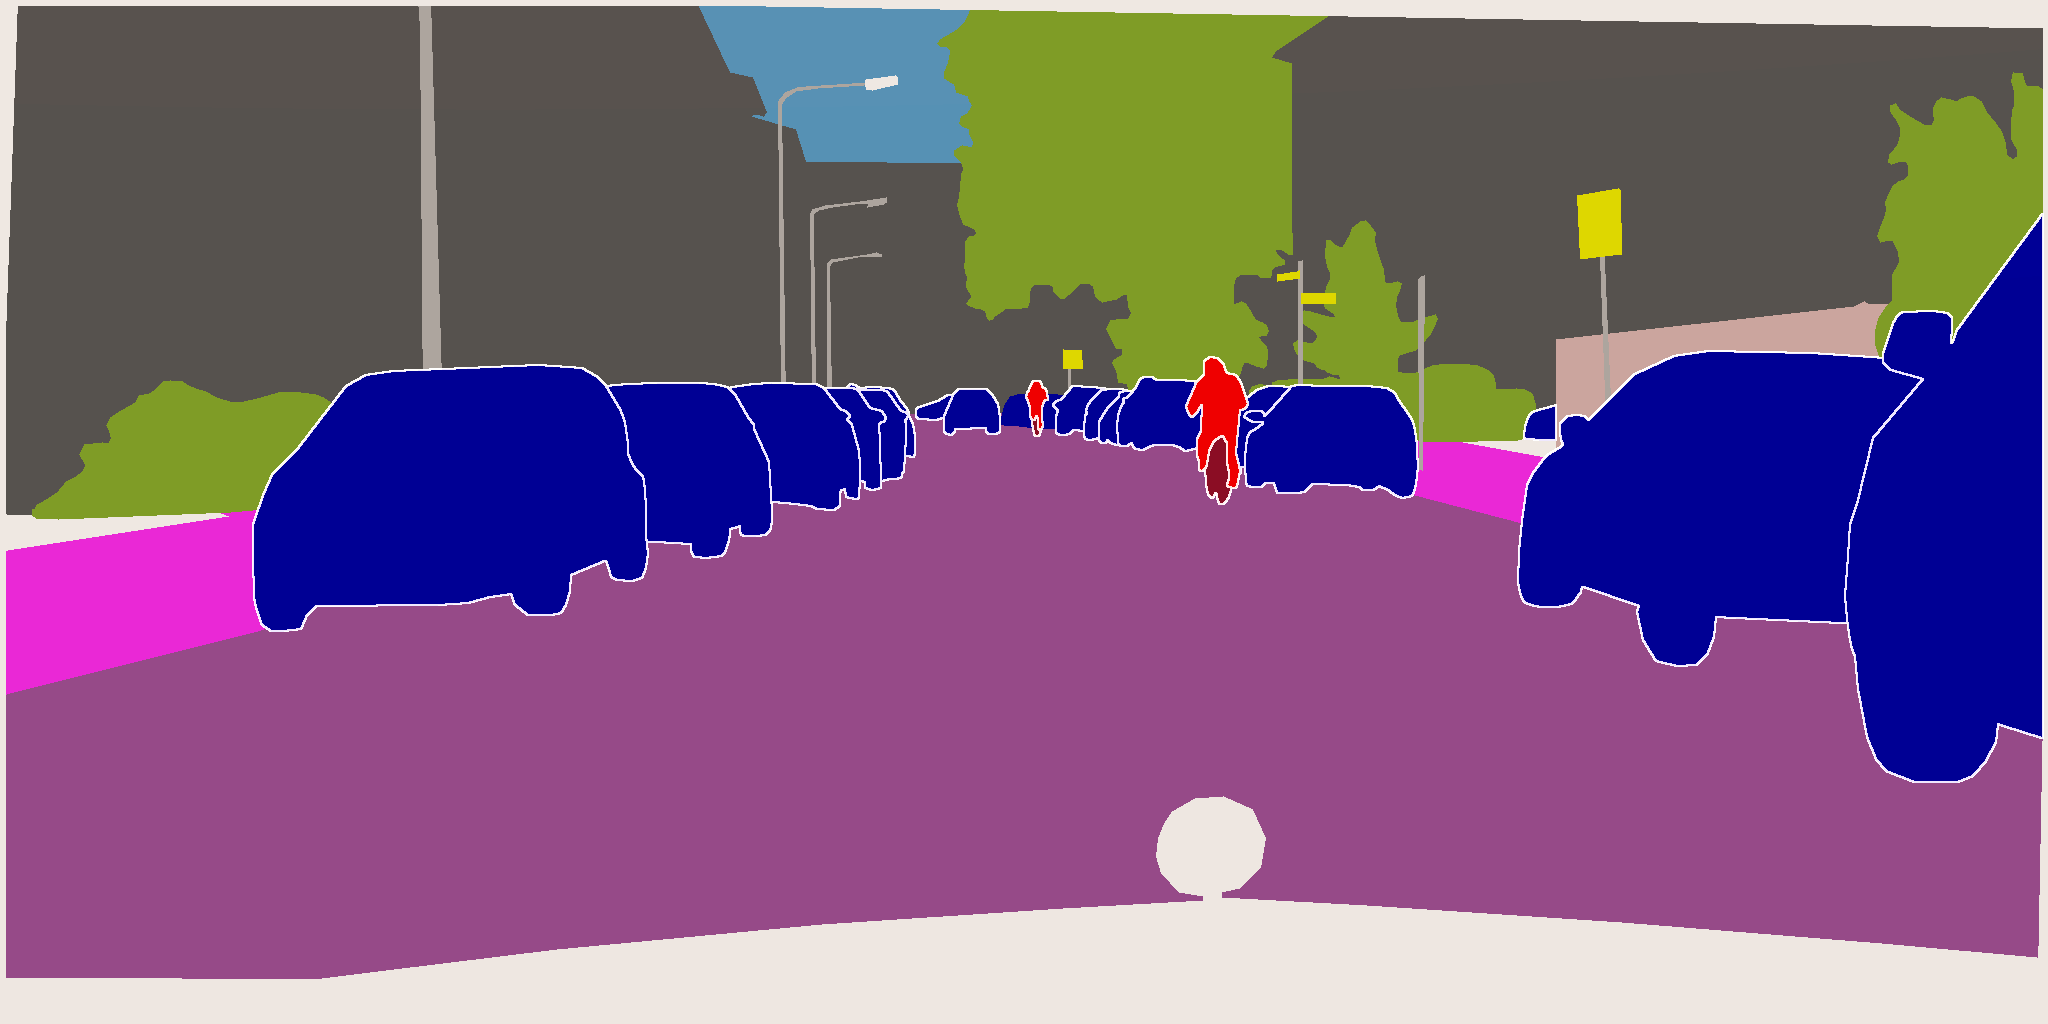
\includegraphics[width = \textwidth / 2 ]{Graphics/Introduction_images/Pansegbright}
        \label{fig:panseg}}
    \caption[Image Segmentation approaches] {Image and corresponding representations a) depicts an RGB image taken from driver's perspective b) shows semantic segmentation of the RGB image c) represents instance segmentation d) shows panoptic segmentation where semantic segmentation and instance segmentation information is represented in a combined fashion \cite{Cordts2015}}
    \label{fig:Rgbseminstseg}
\end{figure}

\textit {Panoptic segmentation} is a recently proposed segmentation task that aims to combine instance and semantic segmentation in a unified segmentation task to generate rich, coherent and comprehensive scene representation \cite{Kirillov2019}. Panoptic segmentation allows for a representation that describes semantic layout as well individual instances appearing in a single view as depicted in \ref{fig:panseg}. Figure \ref{fig:SemsegZoomed}, shows semantic representation of a common urban scenario where each pixel has been assigned to a given class. Although a useful representation that describes a general layout of the scene by separating road, sidewalk, buildings and other traffic participants but it might not suffice for a satisfactory scene interpretation. Highlighted area in the image shows a blob of red coloured pixels that represent people standing on a sidewalk however it can be difficult to argue about number of people and more importantly if some of them intend to cross the road. On the other hand, figure \ref{fig:PanopticsegZoomed} shows combined representation where the people in highlighted region are further separated as individual instances. Such combined representation gives a much detailed information on the scene and can be leveraged by high-level computer vision tasks to argue about behaviour of traffic participants. Autonomous driving as well other computer vision based applications in robotics and medicine can benefit from such rich multi-modal representation for improved image understanding.

Although, both semantic and instance segmentation can complement each other by providing much more detailed information on the scene, they are fundamentally different in the way they are approached and usually require different network architecture topology. Since panoptic segmentation is a unified segmentation task and both of the aforementioned tasks usually rely on features learned using \gls{cnns} it seems a reasonable choice to tailor the architecture by augmenting a common feature extractor. This common feature extractor backbone could learn features that can be utilized by the network to generate instance and semantic segmentation in a combined fashion. Most of the state-of-the-art methods that attempted to solve panoptic segmentation task within a single network either use top-down approaches or proposal based methods such as Mask R-CNN \cite{He2017}. One problem with such two-stage methods is their requirement for an additional region proposal network and furthermore they generate overlapping instance masks with ambiguous instance boundaries which demand additional conflict resolving methods.

\begin{figure}[!ht]
%\centering
    \subfigure[Semantic Segmentation]{
        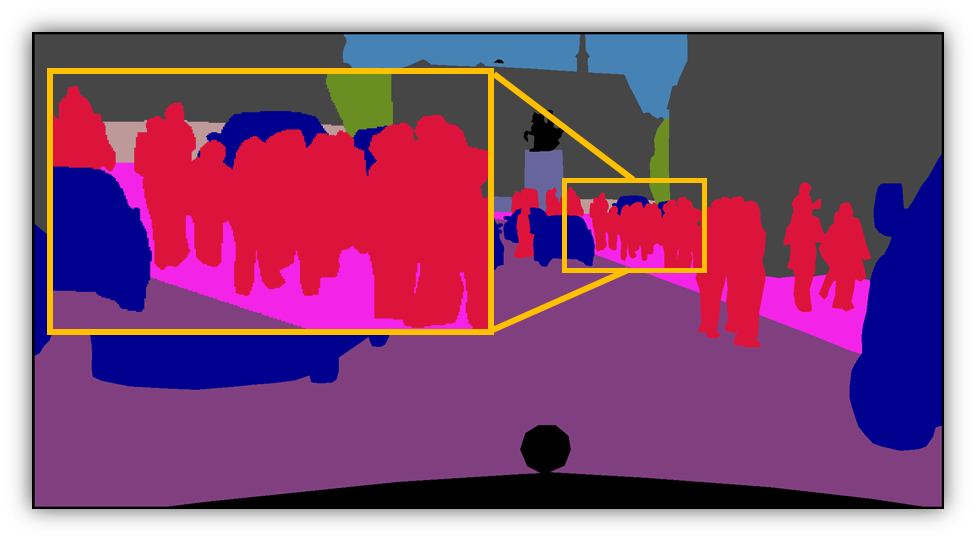
\includegraphics[width = \textwidth / 2 ]{Graphics/Introduction_images/SemsegZoomed.png}
        \label{fig:SemsegZoomed}}
    %\hspace{1pt}
     %add desired spacing between images, e. g. ~, \quad, \qquad, \hfill etc.
     %(or a blank line to force the subfigure onto a new line)
    \subfigure[Panoptic Segmentation]{
        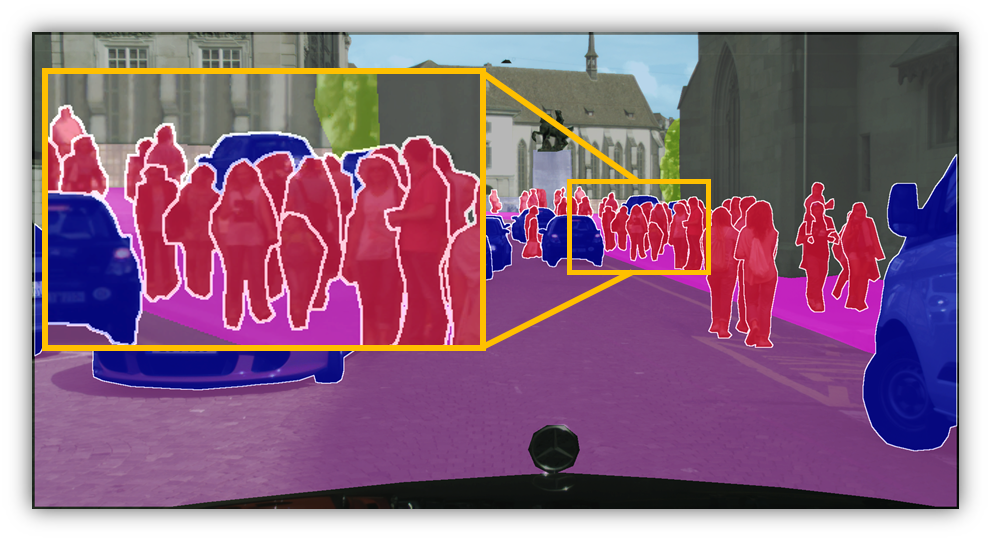
\includegraphics[width = \textwidth / 2 ]{Graphics/Introduction_images/PanopticsegZoomed.png}
        \label{fig:PanopticsegZoomed}}
            \caption[Semantic and Panoptic Segmentation] {Figure shows semantic and panoptic segmentation of an urban scene - highlighting the additional information facilitated by panoptic segmentation a) depicts semantic segmentation of an urban scene b) shows corresponding panoptic segmentation of the scene taken from Cityscapes dataset \cite{Cordts2015}}
\end{figure}





Therefore, it is desired to investigate a simple panoptic segmentation architecture that utilizes dense features extracted from a common backbone feature extractor and makes use of these features to generate both instance and semantic segmentation modalities in a multi-task setting. It is also desired to achieve instance segmentation by exploiting pixel-level relationships whereby learning center points and extent of each instance in one step instead of generating region proposal based overlapping instance masks. 

\section{Problem Statement}

This thesis addresses the task of panoptic segmentation for urban scenarios. The goal
of panoptic segmentation is to assign a unique value, encoding both semantic label and instance id, to every pixel in an image. In panoptic segmentation task, classes are divided into two main categories:

\begin{itemize}
  \item \textit{Stuff}  – amorphous regions of similar texture or material such as sky, building, road.
  \item \textit{Things} – countable objects such as people, cars, bicycles.
\end{itemize}

It is required to identify the class label and extent of each instance of  \textit{things} classes, and only a class labels for all pixels belonging to \textit{stuff} classes. Moreover, it is desired to learn and generate both instance and semantic segmentation modalities within a single network architecture.

In this context, the presented work aims to answer following questions:

\begin{enumerate}

	\item  How to pose two fundamentally diverged approaches in a unified multi-task setting?
	\item  How to represent instances and their pixel-level relationships to generate instance segmentation?

\end{enumerate}

Furthermore, it is desired to investigate instance encoding possibilities and study effects of these representations on overall panoptic segmentation task. 


\section{Outline}
This thesis is structured as follows - Chapter 2 provides a brief overview of fundamentals in semantic, instance and panoptic segmentation. Related work and corresponding literature review has been discussed in chapter 3. In chapter 4, various data representations are introduced and analyzed in the context of pixel-level instance encoding. Subsequently Chapter 5 describes network architecture and experimental setup. In chapter 6, a structured approach to generate panoptic segmentation has been briefly explained. Chapter 7 analyzes the experimental results obtained through these approaches considering both qualitative and quantitative evaluations. Finally, chapter 8 summarizes the thesis and provides an outlook regarding future work.      
% !TeX root = ../thesis.tex

\chapter{Fundamentals}
\label{sec:fundamentals}

This chapter is dedicated to highlighting pre-requisite knowledge in machine learning needed for understanding the contribution and contents of the presented work.
%If not indicated otherwise, fundamentals of neural networks are taken from [blablabla]

\section{Artificial Neural Networks}

\gls{anns}, also commonly referred to as \textit{neural networks} are considered to  be universal function approximators \cite{Hornik1989}. ANNs are machine learning models that are inspired by human brain's biological neural network. A neuron is fundamental computational unit of human brain that is responsible for receiving sensory input via dendrites, process and generate output through axons, see \ref{fig: neuron}. Neurons are therefore the building blocks of brain's inter-connected neural network that processes and transmits information in the form of electrochemical signals. 


\begin{figure}[!htb]
	 \centering 
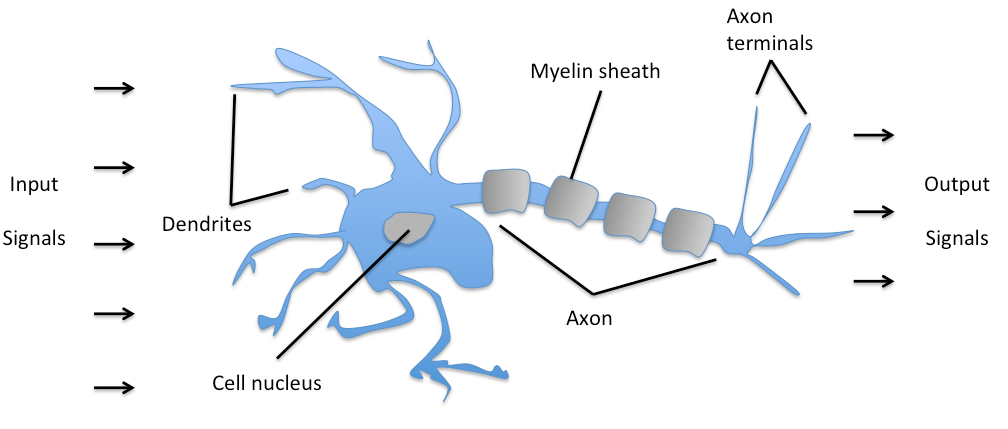
\includegraphics[scale = 0.35]{Graphics/Fundamentals/neuron3x} 
	\caption{Diagram of a biological neuron \cite{RTS20}} 
	\label{fig: neuron} 
\end{figure}

%Although artificial neural networks attempt to simulate characteristics of a biological neural network, state-of-the-art ANNs have never achieved full functional complexity and computational efficiency of their biological counterparts. 


\subsection{Multi-Layer Perceptron}


In 1943, McCulloch and Pitts tried to understand how brain could produce highly complex patterns by using many basic cells that are connected together and presented a simple model \cite{Arbib2004}. In 1958, Frank Rosenblatt proposed a generalized variant of a former, more simple structure to model brain activities by using single layer network \cite{Rosenblatt1958}. 



\begin{figure}[!ht]
	 \centering 
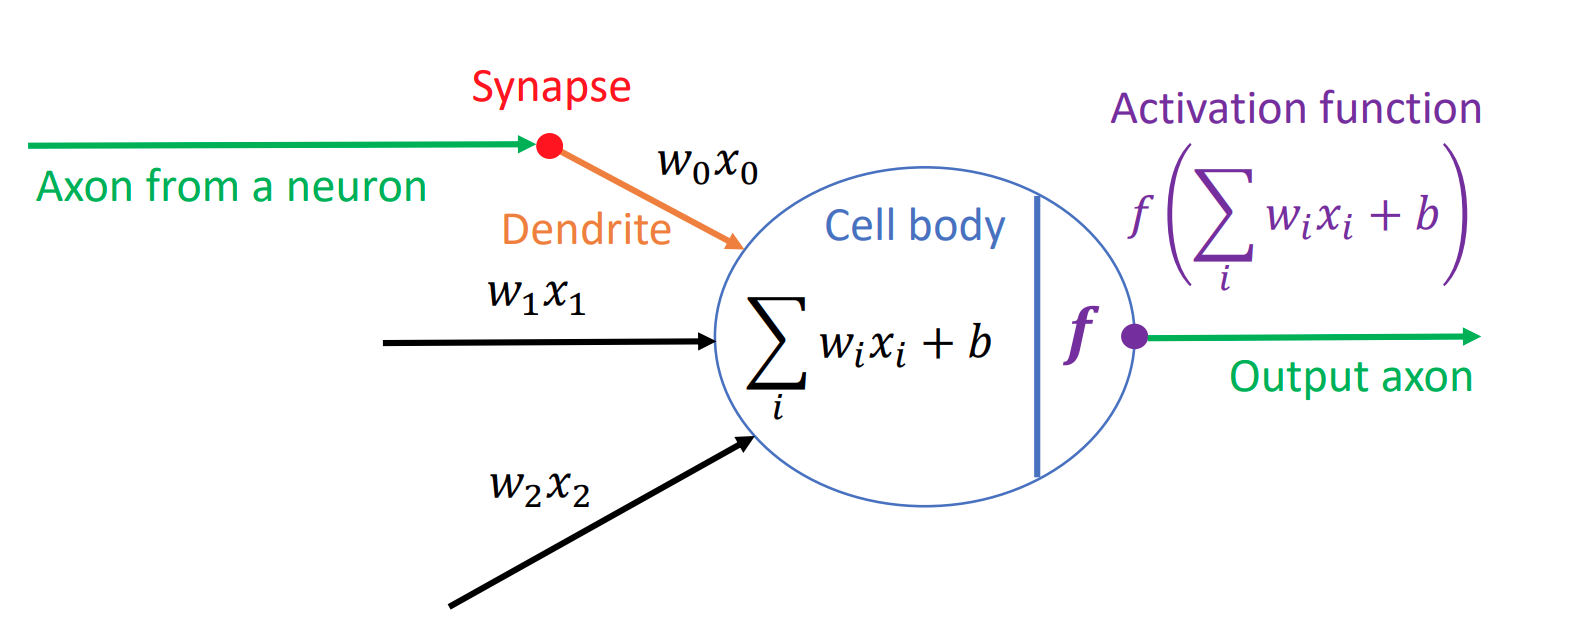
\includegraphics[scale = 0.2]{Graphics/Fundamentals/perceptron1} 
	\caption[Mathematical model of a Perceptron]{Mathematical model of a perceptron. Elements $x_i$ of an input \textbf{x} are multiplied individually with learnable weights $w_i$ and aggregated with an additional learnable bias term. The resultant is processed by a following non-linear activation function $f(.)$ to generate output. \cite{CS231n} }
	\label{fig: perceptron} 
\end{figure}
Structurally, perceptron attempts to replicate the basic phenomenon of receiving multiple input signals and processing them using learnable weights to generate an output.  A perceptron is able to learn weights depending on input-output correspondences, it therefore enables perceptrons to classify information.
As illustrated in \ref{fig: perceptron}, incoming input elements of \textbf{x} are multiplied with corresponding learned weights \textbf{w} (equivalent to a dot product between vectors \textbf{x} and \textbf{w}). Result is then added with another learnable input-independent bias term \textit{b}. 


\begin{equation}a_{\mathbf{x}}=\sum_{i=0} w_{i} x_{i}+b\end{equation}

Final output is generated by passing this weighted sum through a non-linear activation function $f(.)$ which will be explained in a later section in more detail:

%\begin{equation}{\textit{output}}= f\left(\sum_{i} w_{i} x_{i}+b\right)\end{equation}
\begin{equation}{\mathrm{output}}= f\left(\sum_{i=0} w_{i} x_{i}+b\right)\end{equation}


Multiple perceptrons when stacked above each other result in a \textit{layer}, while each perceptron in a layer is referred to as a \textit{node}. Nodes when connected to the nodes of a successive layer in a sequential structure, represent a \gls{mlp}, also known as a \textit{feed-forward neural network} \cite{Svozil1997}. see figure \ref{fig:mlp}.
Number of nodes in a hidden layer define \textit{width} of a network, while model's \textit{depth} is specified by the number of layers chained sequentially to form a neural network structure.

Such a feed forward neural network is used to learn data with multiple features, indicated by  number of input units. Each feature contributes to the output i.e, features are processed independently and information is carried out to the subsequent layers. Node in each layer receives inputs from nodes of preceding layer, processes them by calculating sum of product of each input with corresponding weights and passes the resultant through a non-linear activation function before forwarding to the nodes of following layer. 

Multi-layer structure is an essential modelling feature and furnishes prime contribution. MLP is assumed to learn discriminative features in a hierarchical manner \cite{Goodfellow-et-al-2016}. Lower layers in a network usually learn low-level features, while higher layers build upon these low-level features to generate higher level features. For instance, in digit classification problem, initial layers might discriminate between the presence of straight lines or curves, while higher layers might learn the structural correspondences among theses shapes to discriminate digits. Therefore, it can be loosely compared to a decision tree, where decision for the next stage is based on existence or non-existence of learned features and ultimately final result is built up respecting the features in preceding stages.

\begin{figure}[!ht]
	 \centering 
    %        \includegraphics[scale = 0.30]{Graphics/Fundamentals/mlp_latex}
        \begin{neuralnetwork}[height=5]
            \newcommand{\x}[2]{$x_#2$}
            \newcommand{\y}[2]{$\hat{y}_#2$}
            \newcommand{\hfirst}[2]{\small $h^{(1)}_#2$}
            \newcommand{\hsecond}[2]{\small $h^{(2)}_#2$}
            \inputlayer[count=3, bias=true, title=Input\\layer, text=\x]
            \hiddenlayer[count=4, bias=false, title=Hidden\\layer 1, text=\hfirst] \linklayers
            \hiddenlayer[count=3, bias=false, title=Hidden\\layer 2, text=\hsecond] \linklayers
            \outputlayer[count=2, title=Output\\layer, text=\y] \linklayers
        \end{neuralnetwork}
	\caption[Multi-Layer Perceptron]{Feed forward neural network graph of 3-layer perceptron with 3 input units and a bias term $x_0$, 2 hidden layers and 2 output nodes.The $1^{st}$ and $2^{nd}$ hidden layers contains 4 and 3 hidden units (nodes), respectively \cite{MULTILAYERPERCEPTRON}. }
	\label{fig:mlp} 
\end{figure}


\subsection{Activation Functions}

Activation function is a key component of a neural network since it adds non-linearity in the model. In a perceptron, the weighted sum is a linear combination of the input values. In order to model non-linear functions, it is necessary to allow for non-linearities within the network. Without a non-linearity, network with multiple hidden layers would collapse to network with a single hidden layer. Therefore, the weighted sum is passed through an activation function $f(.)$ before advancing it to a successive layer. Some of the most popular activation functions are \textit{sigmoid function}, \textit{hyperbolic tanget}, \textit{rectified linear or ReLU} and \textit{Leaky ReLU}, see figure \ref{fig:Activation functions}. ReLU - as described by the equation \ref{eq:ReLu}, is however most commonly recommended activation function for deep neural networks since rectifying neurons make for an even better model of biological neurons and yield equal or better performance than hyperbolic tangent and logistic sigmoid activation function based networks \cite{Glorot2011}. 
\begin{equation}f(x)=\left\{\begin{array}{ll}
x & \text { if } x \geq 0 \\
0 & \text { otherwise }
\end{array}\right.
\label{eq:ReLu}
\end{equation}

Compared to \textit{sigmoid or tanh} functions, it has been found to greatly accelerate the convergence of \gls{sgd} \cite{Krizhevsky2017} and does not contain complex computations such as exponential unlike its counterparts.
However, ReLU units are fragile and can “die” due to large gradient flowing through a ReLU neuron could cause the weights to update in such a way that the neuron will never activate again. Leaky ReLUs attempt to fix the aforementioned problem of ``dying ReLU" by having a small negative slope about $0.01$ insted of zero in regime $(x<0)$, see equation \ref{eq:LeakyReLu} \cite{CS231n}.
\begin{equation}f(x)=\left\{\begin{array}{ll}
0.01 & \text { for } x<0 \\
1 & \text { for } x \geq 0
\end{array}\right.
\label{eq:LeakyReLu}
\end{equation}

\begin{figure}[!ht]
%\centering
    \subfigure[sigmoid function]{
        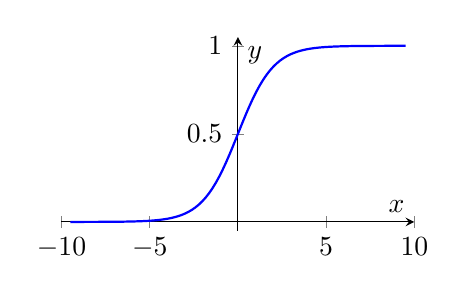
\begin{tikzpicture}
            \begin{axis}[
                axis lines=middle,
                xmax=10,
                xmin=-10,
                ymin=-0.05,
                ymax=1.05,
                xlabel={$x$},
                ylabel={$y$}, width = \textwidth /2, height = \textwidth / 3
            ]
            \addplot [domain=-9.5:9.5, samples=100,
                      thick, blue] {1/(1+exp(-x)};
            \end{axis}
        \end{tikzpicture}
    \label{fig:sigmoid}}
    \hfill
     %add desired spacing between images, e. g. ~, \quad, \qquad, \hfill etc.
     %(or a blank line to force the subfigure onto a new line)
    \subfigure[tanh function]{
       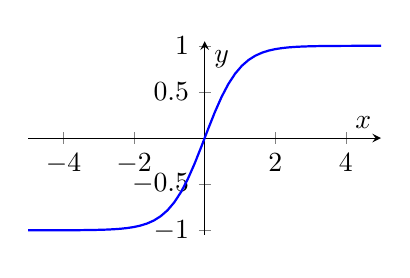
\begin{tikzpicture}
            \begin{axis}[
                axis lines=middle,
                xmax=5,
                xmin=-5,
                ymin=-1.05,
                ymax=1.05,
                xlabel={$x$},
                ylabel={$y$}, width = \textwidth /2, height = \textwidth / 3]
            \addplot [domain=-9.5:9.5, samples=100,
                 thick, blue] {(exp(x) - exp(-x))/(exp(x) + exp(-x))};
            \end{axis}
        \end{tikzpicture}
    \label{fig:tanh}}
    %\hspace{10pt}
    \subfigure[ReLU]{
        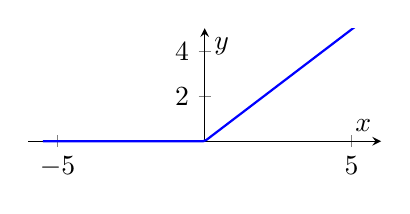
\begin{tikzpicture}
            \begin{axis}[
                axis lines=middle,
                xmax=6,
                xmin=-6,
                ymin=-0.05,
                ymax=5.05,
                xlabel={$x$},
                ylabel={$y$}, width = \textwidth /2, height = \textwidth / 4]
            \addplot [domain=-5.5:5.5, samples=100, thick, blue] {max(0, x)};
            \end{axis}
        \end{tikzpicture}
    \label{fig:ReLU}}
    \hfill
    \subfigure[Leaky ReLU]{
        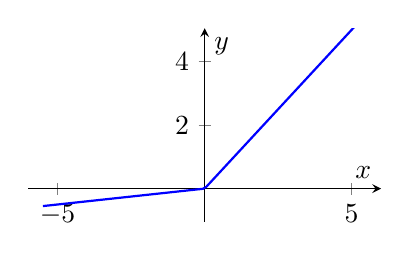
\begin{tikzpicture}
            \begin{axis}[
                axis lines=middle,
                xmax=6,
                xmin=-6,
                ymin=-1.05,
                ymax=5.05,
                xlabel={$x$},
                ylabel={$y$},  width = \textwidth /2, height = \textwidth / 3]
            \addplot [domain=-5.5:5.5, samples=100,
                  thick, blue] {max(0.1 * x, x)};
        \end{axis}
    \end{tikzpicture}
    \label{fig:Leaky ReLU}}
    \caption[Characteristic curves for activation functions]{Characteristic curves for Activation Functions a) sigmoid - $output=\frac{1}{1+e^{-x}}$  b) hyperbolic tanget - $output=\frac{e^{x}-e^{-x}}{e^{x}+e^{-x}}$ c) rectified linear (ReLU) - $output=\max (0, x)$  d) Leaky ReLU - $output=\max (0.01 \times x, x)$ \cite{FUNCTIONS}}
    \label{fig:Activation functions}
\end{figure}


\subsection{Optimization}
\label{subsec:learningnopt}
This section is dedicated to brief description of the learning process within a neural network.
In supervised learning, network learns from multiple sets of input-groundtruth $($\textbf{x}$, y_{gt})$ pairs commonly known as \textit{training set} in an iterative process. To this end, backpropogation method is employed to update the weights \textbf{w} \textit{(learning)} according to a performance measure of network in each step.

When an input \textbf{x} is fed into such a \textit{feed-forward neural network}, it sequentially multiplies input elements $x_i$ with corresponding randomly initialised weights \textbf{w} until the \textit{output layer}, which generates the final predicted output $\hat{y}$. This output is then compared against the corresponding groudtruth label, objective is to update the network parameters $\mathbf{w}$ according to how ``incorrect" network was in its prediction. A common comparison criterion is \textit{Mean Squared Error} (MSE) - which as the name suggest is the mean of squared difference between the predicted $\hat{y}$ and groundtruth value $ y_{gt}$. Mathematically, it can be written as:
\begin{equation}L\left(\mathbf{w}, \mathbf{x}, \mathbf{y}_{\mathbf{gt}}\right)=\frac{1}{N} \sum_{\mathbf{i}}^{N}\left(\hat{y}_{i}(\mathbf{w}, \mathbf{x})-y_{gt, i}\right)^{2}\label{eq:mse}
\end{equation}

%Since, it is a common practice to find the loss for a certain subset of training set instead of every single sample %independently. Equation \ref{eq:mse} corresponds to MSE of a subset. 
The loss \textit{L} is low if the prediction is similar to the groundtruth value, and higher if dissimilar. The goal is then to minimize this \textit{loss function L} which in this case is, MSE based.
To minimize this loss, each parameter of $\mathbf{w}$ of the hidden layers of
the neural network is tuned such that it aids in lowering the overall difference between predicted and corresponding groundtruth values. \textit{Objective function} for minimising the loss then can be written as : 

\begin{equation}
\min _{\mathbf{w}} L\left(\mathbf{w}, \mathbf{x}, \mathbf{{y}_{\mathbf{gt}}}\right)
\end{equation}

This can be achieved by calculating the gradient of loss with respect to parameters and changing the current weights $\mathbf{w_{t}}$ such that the new weights $\mathbf{w_{t + 1}}$ result in minimum loss. Essentially, it is intended to select the weights in descent direction of the gradient:

\begin{equation}
- \frac{\delta}{\delta \mathbf{w}} L\left(\mathbf{w}, \mathbf{x}, \mathbf{y}_{\mathbf{gt}}\right)
\end{equation}

Since, the loss depends upon all the weights $\mathbf{w}$ and biases $\mathbf{b}$ in all hidden layers, it is important to calculate gradients with respect to all trainable dependent variables normally calculated using \textit{backpropagation algorithm} \cite{Svozil1997} which exploits chain-rule :
\begin{equation}\frac{d y}{d x}=\frac{d y}{d u} \frac{d u}{d x}\end{equation}

The derivatives for all the variables is calculated using back-propagation  algorithm by recursive application of chain-rule, the weights are then updated \textit{(learning)} using commonly employed \gls{gd} \cite{Goodfellow-et-al-2016}:

\begin{equation}\mathbf{w}_{\mathbf{t}_{\mathbf{i}+1}}=\mathbf{w}_{\mathbf{t}}-\gamma_{t_{i}} \frac{\delta}{\delta \mathbf{w}_{\mathbf{t}_{\mathbf{i}}}} L\left(\mathbf{w}_{\mathbf{t}_{\mathbf{i}}}, \mathbf{x}_{\mathbf{t}_{\mathbf{i}}}, \mathbf{y}_{\mathbf{g} \mathbf{t}, \mathbf{t}_{\mathbf{i}}}\right)\end{equation}


$\gamma_{t_{i}}$ is the \textit{learning rate} which represents how fast the network weights are adapted with respect to gradient.

\gls{sgd} is an incremental version of vanilla \gls{gd} which uses a subset of training set at each step instead of whole trainig set which has the benefit of faster convergence and generalization \cite{Rumelhart1986}. \textit{Adam}, is another commonly used optimizer which uses adaptive learning rate and has the advantage of better convergence due to adaptive nature \cite{Goodfellow-et-al-2016}. In the presented work, Adam has been employed as an optimizer during trainings.

\section{Convolutional Neural Network}

It can be observed that for larger dimensional inputs a classical artificial neural network \gls{anns} explodes in term of memory requirements. Consider an image with $200\times200$ spatial resolution and an ANN with $10$ \textit{nodes} in the first layer, the parameters end up being $200000$ for this layer only. Memory requirement is a problem but also the local co-relations are not taken into account, instead all the pixels are equally co-related leading to a lot of redundancy, slow optimisation and inference times. \textit{Convolutional Neural Networks} (CNNs), therefore are variant of ANNs that are well-suited for grid-like structured and spatially co-related data. 
\bigskip

\begin{figure}[!ht]
	 \centering 
        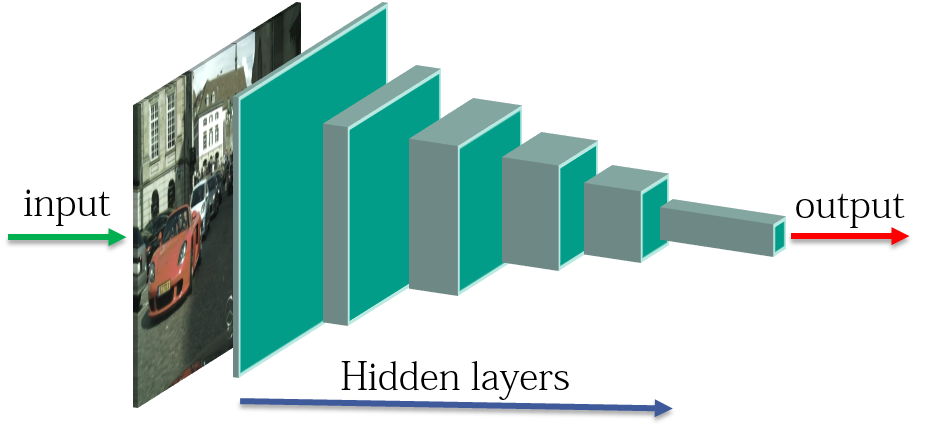
\includegraphics[scale = 0.7]{Graphics/Fundamentals/CNN.png} 
	\caption[Convolutional Neural Network]{Visualisation of a convolutional neural network with $5$ hidden layers}
	\label{fig: CNN} 
\end{figure}

\subsection{Convolution Operator}
Convolutional Neural Networks (\gls{cnns}) make use of \textit{convolution operator}. Convolution operations alleviate the problem of redundancy by re-using the same kernel over spatial dimensions and also model local co-relations across pixels. Since, \gls{cnns} respect the local spatial co-relations and are also memory efficient due to weight sharing properties. Therefore, CNNs are widely used for learning image based data for computer vision applications.

Convolution is an operation on two functions \textit{I} and \textit{K}, which produces a third function that can be interpreted as a filtered (``convolved") version of \textit{I}. \cite{SpatialConv}

\begin{equation}I[x, y] * K[x, y]=\sum_{m=-\infty}^{\infty} \sum_{n=-\infty}^{\infty} I\left[m, n\right] \cdot K\left[x-m, y-n\right]\end{equation}

Visualisation of such a 2D- convolution between an image and a kernel of size $3\times3$ can be seen in the figure \ref{fig:Conv} where a filter is applied across spatial dimension of the image to generate a filtered version of input image.


\begin{figure}[!ht]
	 \centering 
    %        \includegraphics[scale = 0.30]{Graphics/Fundamentals/mlp_latex}
        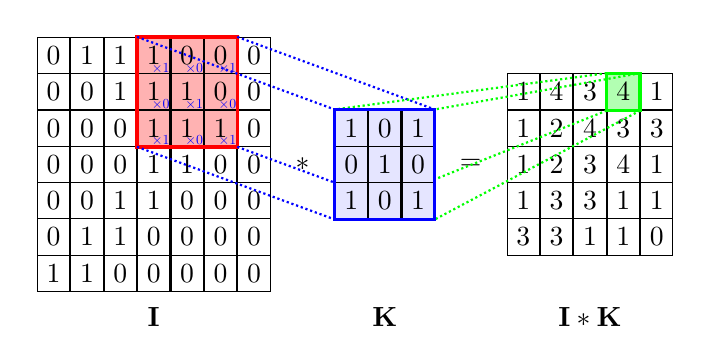
\begin{tikzpicture}

        	\matrix (mtr) [matrix of nodes,row sep=-\pgflinewidth, nodes={draw}]
        	{
        		0 & 1 & 1 & |[fill=red!30]| 1 & |[fill=red!30]| 0 & |[fill=red!30]| 0 & 0\\
        		0 & 0 & 1 & |[fill=red!30]| 1 & |[fill=red!30]| 1 & |[fill=red!30]| 0 & 0\\
        		0 & 0 & 0 & |[fill=red!30]| 1 & |[fill=red!30]| 1 & |[fill=red!30]| 1 & 0\\
        		0 & 0 & 0 & 1 & 1 & 0 & 0\\
        		0 & 0 & 1 & 1 & 0 & 0 & 0\\
        		0 & 1 & 1 & 0 & 0 & 0 & 0\\
        		1 & 1 & 0 & 0 & 0 & 0 & 0\\
        	};
        
        	\draw[very thick, red] (mtr-1-4.north west) rectangle (mtr-3-6.south east);
        
        	\node [below= of mtr-5-4.south] (lm) {$\mathbf{I} $};
        
        	\node[right = 0.2em of mtr] (str) {$*$};
        
        	\matrix (K) [right=0.2em of str,matrix of nodes,row sep=-\pgflinewidth, nodes={draw, fill=blue!30}]
        	{
        		1 & 0 & 1 \\
        		0 & 1 & 0 \\
        		1 & 0 & 1 \\
        	};
        	\node [below = of K-3-2.south] (lk) {$\mathbf{K} $};
        
        	\node [right = 0.2em of K] (eq) {$=$};
        
        	\matrix (ret) [right=0.2em of eq,matrix of nodes,row sep=-\pgflinewidth, nodes={draw}]
        	{
        		1 & 4 & 3 & |[fill=green!30]| 4 & 1\\
        		1 & 2 & 4 & 3 & 3\\
        		1 & 2 & 3 & 4 & 1\\
        		1 & 3 & 3 & 1 & 1\\
        		3 & 3 & 1 & 1 & 0\\
        	};
        	\node [below = of ret-4-3.south] (lim) {${\mathbf{I} } * {\mathbf{K} }$};
        
        	\draw[very thick, green] (ret-1-4.north west) rectangle (ret-1-4.south east);
        
        	\draw[densely dotted, blue, thick] (mtr-1-4.north west) -- (K-1-1.north west);
        	\draw[densely dotted, blue, thick] (mtr-3-4.south west) -- (K-3-1.south west);
        	\draw[densely dotted, blue, thick] (mtr-1-6.north east) -- (K-1-3.north east);
        	\draw[densely dotted, blue, thick] (mtr-3-6.south east) -- (K-3-3.south east);
        
        	\draw[densely dotted, green, thick] (ret-1-4.north west) -- (K-1-1.north west);
        	\draw[densely dotted, green, thick] (ret-1-4.south west) -- (K-3-1.south west);
        	\draw[densely dotted, green, thick] (ret-1-4.north east) -- (K-1-3.north east);
        	\draw[densely dotted, green, thick] (ret-1-4.south east) -- (K-3-3.south east);
        
        	\matrix (K) [right=0.2em of str,matrix of nodes,row sep=-\pgflinewidth, nodes={draw, fill=blue!10}]
        	{
        		1 & 0 & 1 \\
        		0 & 1 & 0 \\
        		1 & 0 & 1 \\
        	};
        
        	\draw[very thick, blue] (K-1-1.north west) rectangle (K-3-3.south east);
        
        	\node[anchor=south east, inner sep=0.01em, blue] at (mtr-1-4.south east) (xx) {\scalebox{.5}{$\times 1$}};
        	\node[anchor=south east, inner sep=0.01em, blue] at (mtr-1-5.south east) (xx) {\scalebox{.5}{$\times 0$}};
        	\node[anchor=south east, inner sep=0.01em, blue] at (mtr-1-6.south east) (xx) {\scalebox{.5}{$\times 1$}};
        	\node[anchor=south east, inner sep=0.01em, blue] at (mtr-2-4.south east) (xx) {\scalebox{.5}{$\times 0$}};
        	\node[anchor=south east, inner sep=0.01em, blue] at (mtr-2-5.south east) (xx) {\scalebox{.5}{$\times 1$}};
        	\node[anchor=south east, inner sep=0.01em, blue] at (mtr-2-6.south east) (xx) {\scalebox{.5}{$\times 0$}};
        	\node[anchor=south east, inner sep=0.01em, blue] at (mtr-3-4.south east) (xx) {\scalebox{.5}{$\times 1$}};
        	\node[anchor=south east, inner sep=0.01em, blue] at (mtr-3-5.south east) (xx) {\scalebox{.5}{$\times 0$}};
        	\node[anchor=south east, inner sep=0.01em, blue] at (mtr-3-6.south east) (xx) {\scalebox{.5}{$\times 1$}};

        \end{tikzpicture}

	\caption[Visualisation of 2D Convolution Operation]{Visualisation of a 2D-convolution operation between Image \textit{I} and $3\times3$ kernel \textit{K} where \textit{I * K} represents the result after operation. \cite{MATCONV} }
	\label{fig:Conv} 
\end{figure}

It can also be seen from the figure \ref{fig:Conv} that spatial resolution of output is smaller than the input due to nature of convolution operation which results in reduced features in output. To remedy this effect, input is padded across the borders with extra 0s. Additionally, non-linearity such as ReLU as mentioned in \ref{eq:ReLu} is employed after convolution operations to avoid network from collapsing to a linear model. Therefore, each layer in a CNN has following parameters:

\begin{itemize}
    \item Number of filter kernels - N
    \item Spatial resolution of kernel - K
    \item Number of pixels, filter strides between two applications - S
    \item Number of zeros padded around the borders - P
\end{itemize}

Given the parameters, output dimensions of a convolutional layer in a CNN can be calculated as follows:

\begin{equation} H_{\text {output}}=\frac{H_{\text {input}}-K+2 P}{S}+1\label{eq:hout}\end{equation}
\begin{equation} W_{\text {output}}=\frac{W_{\text {input}}-K+2 P}{S}+1\label{eq:wout}\end{equation}
\begin{equation}D_{\text {output}}=N\label{eq:dout}\end{equation}

In the equations \ref{eq:hout} - \ref{eq:dout}, $H_{output}$, $W_{output}$ and $D_{output}$ correspond to height, width and depth size of the output from convolutional layer.


\subsection{Pooling Operator}

\label{subsec: pooling_operation}

From figure \ref{fig:Conv}, it can be seen that the depth of output is usually increased relative to the input which leads to an increase in the values calculated during the forward pass, even modern Graphics Processing Units (GPUs) might not be able to hold them in memory specially if the \gls{cnns} is very deep - has large number of layers. To avoid this computational expense, pooling operations are used to reduce the spatial dimensions of calculated feature outputs while keeping necessary information.

Pooling operation also helps in improving generalization by considering translational in-variances of features calculated in a convolutional layer.

Pooling is a spatial down-sampling operation with two variations:

\begin{itemize}
    \item Max-pooling  - from a spatial window of $K$ x $K$, maximum value is picked
    \item Average-pooling - from a spatial window of $K$ x $K$, average value is calculated 
\end{itemize}


 \begin{figure}[!ht]
	 \centering 
        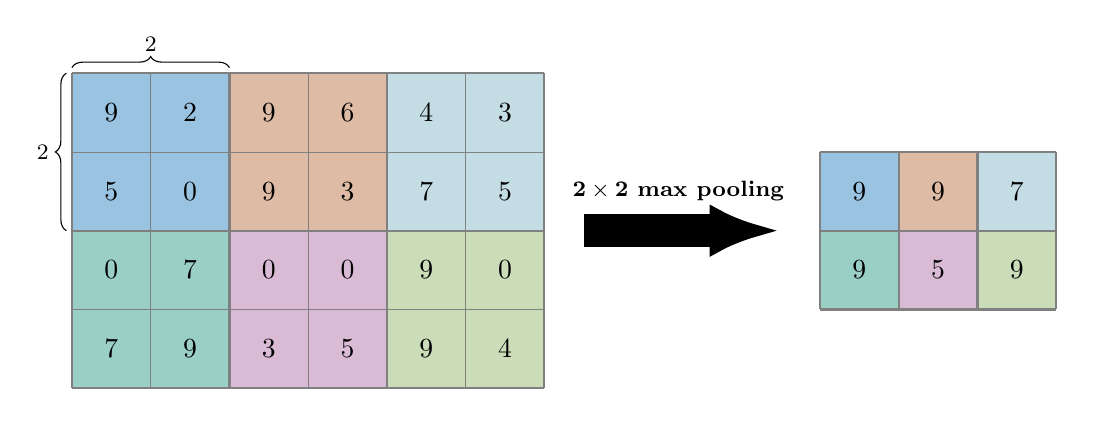
\begin{tikzpicture}
            \fill [c1] (0, 0) rectangle (2, 2);
            \fill [c2]   (2, 0) rectangle (4, 2);
            \fill [c3]  (4, 0) rectangle (6, 2);
            \fill [c4] (0, 2) rectangle (2, 4);
            \fill [c5]   (2, 2) rectangle (4, 4);
            \fill [c6]   (4, 2) rectangle (6, 4);
        
            \fill [c1]  (9.5, 1) rectangle (10.5, 2);
            \fill [c2]   (10.5, 1) rectangle (11.5, 2);
            \fill [c3]  (11.5, 1) rectangle (12.5, 2);
            \fill [c4]  (9.5, 2) rectangle (10.5, 3);
            \fill [c5]   (10.5, 2) rectangle (11.5, 3);
            \fill [c6]   (11.5, 2) rectangle (12.5, 3);
        
            \foreach \i in {\xMin,...,\xMax} {
                \draw [very thin,gray] (\i,\yMin) -- (\i,\yMax)  node [below] at (\i,\yMin) {};
            }
            \foreach \i in {\yMin,...,\yMax} {
                \draw [very thin,gray] (\xMin,\i) -- (\xMax,\i) node [left] at (\xMin,\i) {};
            }
        
            \foreach \i in {\xMin,2,...,\xMax} {
                \draw [thick,gray] (\i,\yMin) -- (\i,\yMax)  node [below] at (\i,\yMin) {};
            }
            \foreach \i in {\yMin,2,...,\yMax} {
                \draw [thick,gray] (\xMin,\i) -- (\xMax,\i) node [left] at (\xMin,\i) {};
            }
            \node at (0.5, 0.5) {7};
            \node at (1.5, 0.5) {9};
            \node at (2.5, 0.5) {3};
            \node at (3.5, 0.5) {5};
            \node at (4.5, 0.5) {9};
            \node at (5.5, 0.5) {4};
            %
            \node at (0.5, 1.5) {0};
            \node at (1.5, 1.5) {7};
            \node at (2.5, 1.5) {0};
            \node at (3.5, 1.5) {0};
            \node at (4.5, 1.5) {9};
            \node at (5.5, 1.5) {0};
            %
            \node at (0.5, 2.5) {5};
            \node at (1.5, 2.5) {0};
            \node at (2.5, 2.5) {9};
            \node at (3.5, 2.5) {3};
            \node at (4.5, 2.5) {7};
            \node at (5.5, 2.5) {5};
            %
            \node at (0.5, 3.5) {9};
            \node at (1.5, 3.5) {2};
            \node at (2.5, 3.5) {9};
            \node at (3.5, 3.5) {6};
            \node at (4.5, 3.5) {4};
            \node at (5.5, 3.5) {3};
        
            \draw[draw=black,line width=12pt,-{Latex[length=9mm]}] (6.5, 2)  -- (9,2);
            \node[font=\footnotesize\bfseries] at (7.7, 2.5) {$\mathbf{2\times 2}$ max pooling};
        
            \foreach \i in {\xMinR,...,\xMaxR} {
                \draw [thick,gray] (\i,\yMinR) -- (\i,\yMaxR)  node [below] at (\i,\yMinR) {};
            }
            \foreach \i in {\yMinR,...,\yMaxR} {
                \draw [thick,gray] (\xMinR,\i) -- (\xMaxR,\i) node [left] at (\xMinR,\i) {};
            }
        
            \node at (10, 1.5) {9};
            \node at (11, 1.5) {5};
            \node at (12, 1.5) {9};
            \node at (10, 2.5) {9};
            \node at (11, 2.5) {9};
            \node at (12, 2.5) {7};
        
            \draw [decorate,decoration={brace,amplitude=4pt},xshift=-2pt,yshift=0pt]
        (0,2) -- (0,4) node [black,midway,xshift=-0.3cm] {\footnotesize $2$};
        
            \draw [decorate,decoration={brace,amplitude=4pt},xshift=0pt,yshift=2pt]
        (0,4) -- (2,4) node [black,midway,yshift=+0.3cm] {\footnotesize $2$};
        \end{tikzpicture}
    	\caption[Max Pooling Operation]{Visualisation of a 2x2 max-pooling operation \cite{MAXPOOLING}}
	\label{fig: maxpooling} 
\end{figure}

Figure \ref{fig: maxpooling} shows a 2D- max-pooling operation, where maximum value is pooled using a kernel window of size $2$x$2$ and stride $2$. Both max and average pooling have their own advantages, latter also known as \textit{mean pooling}. However, experiments have shown that max pooling is more likely to yield better results when used in \gls{cnns} \cite{Scherer2010}. 




\subsection{Depth-wise Separable Convolutions}

Previously described convolution operation in \ref{fig:Conv} is a simple case for a single channel input. However, learning on an RGB images or performing convolution operations in higher layers of CNN requires extension of kernel by adding additional channels such that, channels of filters equal the channels of input. Consider a $10$-channel input and a required output depth of $20$- channels with a kernel window of $7$x$7$ will result in over $9800$ learnable parameters in single layer. Having this many number of parameter is a high computational cost and might result in over-fitting.

Considering the above facts, \textit{inception modules} provides for more efficient computations and deeper network architecture through dimensionality reduction with stacked $1$x$1$ convolutions (also known as \textit{point-wise} convolutions) before spatial convolutions. This is equivalent to looking at cross-channel co-relations, prior to mapping the input data into 3 or 4 separate channel spaces that are smaller than the original input space, and then concatenating them into 3D spaces\cite{DBLPI:journals/corr/SzegedyLJSRAEVR14}.

Recently proposed \textit{Xception modules} \cite{DBLP:journals/corr/Chollet16a} attempts to improve Inception modules by using \textit{depth-wise separable convolutions} - a spatial convolution performed independently over each channel of an input, followed by a point-wise $1$x$1$ convolution, projecting the channels output onto a new channel space \cite{DBLPMNv1:journals/corr/HowardZCKWWAA17}. See fig \ref{fig: depthwiseseperableconv} for reference. Therefore, improving efficiency of convolution operations without extra computational overhead.
  

\begin{figure}[!ht]
	 \centering 
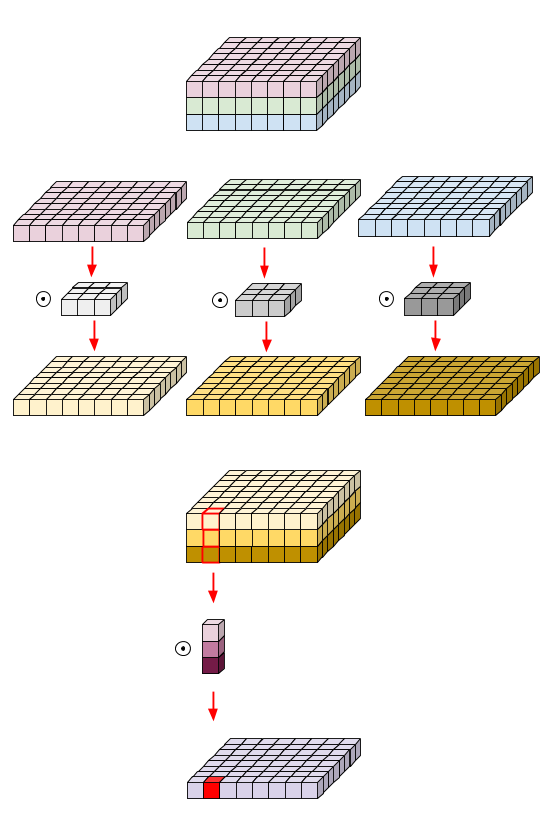
\includegraphics[scale = 0.6
]{Graphics/Fundamentals/Depthwise_seperable_convolution} 
	\caption[Depth-wise Separable Convolution]{Depiction of Depth-wise separable convolution - depthwise convolution, followed by a point-wise convolution \cite{DEPTHWISESEPCONV}}
	\label{fig: depthwiseseperableconv} 
\end{figure}



\subsection{Atrous Convolutions}
One of the challenges in solving tasks such as semantic segmentation using deep convolutional neural networks (DCNNs),  is reduced spatial feature resolution as seen in figure \ref{fig: CNN}. Since, it is desired to generate an output of spatial resolution exactly equal to the input size, it maybe favourable to generate detailed spatial information. \textit{Atrous convolutions} have proved to be a powerful tool that allow for adjusting filter’s field-of-view as well as controlling the resolution of features computed using DCNNs, specially for semantic image segmentation \cite{Chen2018dlv3}.

\begin{figure}[!ht]
	 \centering 
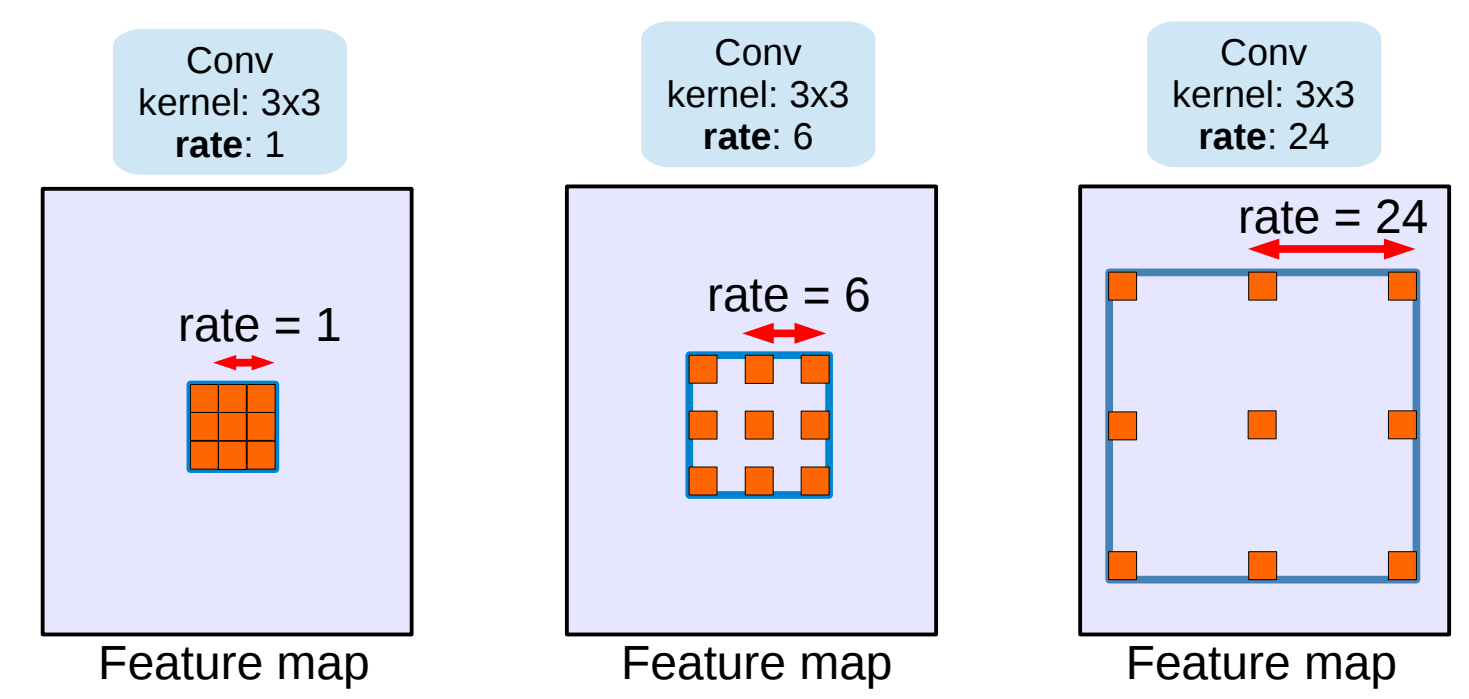
\includegraphics[scale = 0.25]{Graphics/Fundamentals/AtrousConvolution} 
	\caption[Atrous Convolutions]{Visualisation of atrous convolution filters overlayed on feature map, showing changing field of view at rate 1, 6, 24 - while maintaining number of parameters \cite{Deeplabv3+:journals/corr/abs-1802-02611}}
	\label{fig: atrousconv} 
\end{figure}

Atrous convolutions have also been referred to as \textit{dilated convolutions} in literature \cite{Yu2016MultiScaleCA}. Such convolutions introduce additional parameter to convolutional layers called \textit{dilation/atrous rate} $\mathbf{r}$. This defines a spacing by padding zeros between learnable values in a kernel. Therefore, a 3x3 kernel with a dilation rate of 2 will have the same effective field of view as a $5\times5$ kernel, while only using 9 parameters. Consider one-dimensional input feature map \textit{\textbf{x}}, a kernel \textit{\textbf{k}} and for each location \textit{\textbf{i}} on the output feature map \textit{\textbf{y}}, atrous convolution can be mathematically defined as follows:

\begin{equation}\boldsymbol{y}[\boldsymbol{i}]=\sum_{\boldsymbol{n}} \boldsymbol{x}[\boldsymbol{i}+r \cdot \boldsymbol{n}] \boldsymbol{k}[\boldsymbol{n}]\end{equation}

where \textit{r} is the atrous rate. Standard convolution can then be seen as a special case of atrous convolution with atrous rate = $1$.  


\subsection{Atrous Separable Convolutions}
\label{subsec:atroussepconv}
\textit{Atrous separable convolutions} or \textit{atrous depth-wise separable convolutions} are depth-wise separable convolutions that make use of atrous rates, see figure \ref{fig: atroussepconv}.
Since depth-wise separable convolutions have shown to be efficient in terms of number of parameters while maintaining performance and atrous convolutions allow for explicit control of spatial resolution of computed features therefore a combination of both can be exploited for semantic segmentation problems. It has been shown that atrous separable convolution significantly
reduces the computation complexity while maintaining similar (or better) performance \cite{Deeplabv3+:journals/corr/abs-1802-02611}.

\begin{figure}[!ht]
	 \centering 
        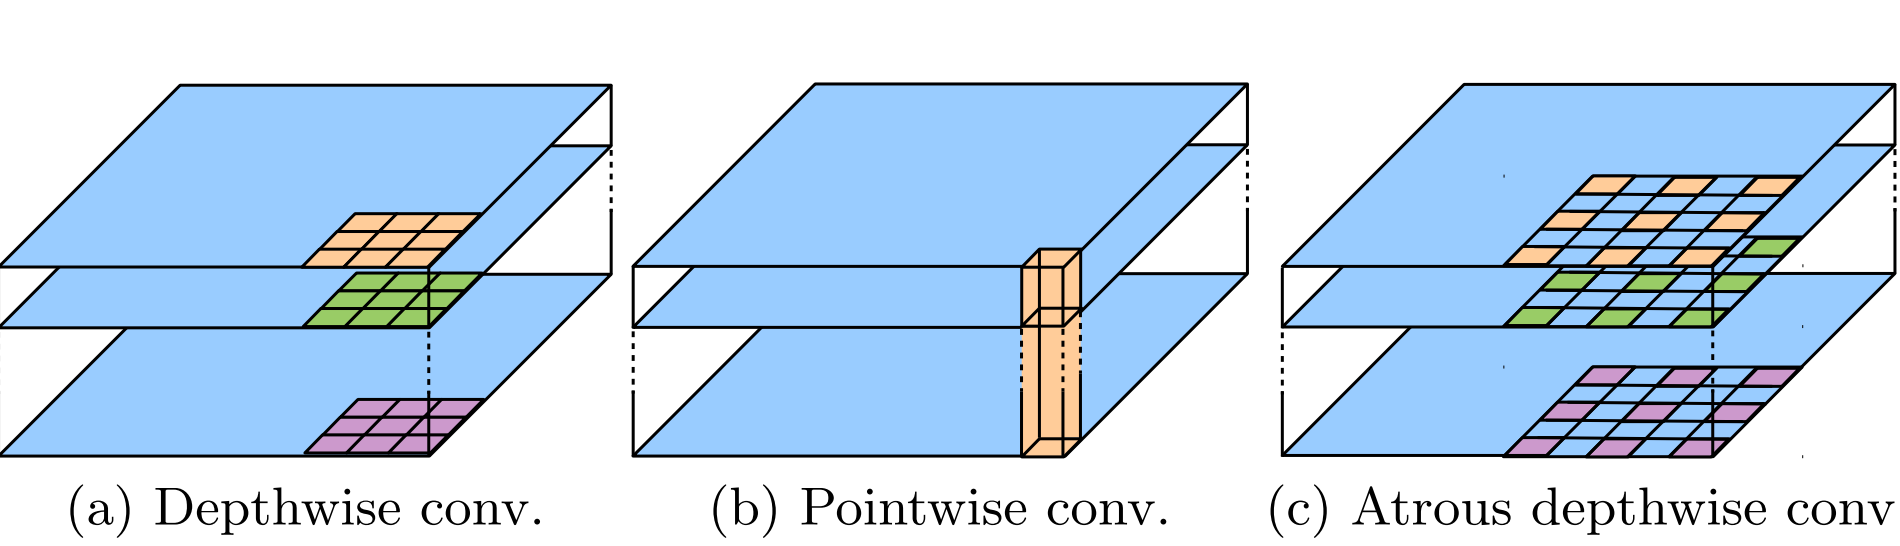
\includegraphics[scale=0.26]{Graphics/Fundamentals/AtrousSeperableConv}
	    \caption[Atrous Seperable Convolutions]{Visualisation of different convolutions - a) depthwise separable convolution b) point-wise convolution c) atrous depthwise seperable convolution \cite{Deeplabv3+:journals/corr/abs-1802-02611}}
	\label{fig: atroussepconv} 
\end{figure}



\newpage
\section{Distance Transform}
It is desired to learn pixel-level relationships to represent instances and learn these representations using a deep convolutional neural network. One way to describe these relationships is relative position with respect to center of object. Since, instances appearing in driver's perspective camera can be heavily occluded by other instances, it is therefore required that these representations are robust and persistent. To deal with occlusions, instead of physical center, \textit{center of mass} is used, making it tolerant to occlusions by considering the center of visible part of instance. To this end, \textit{distance transform} is employed to calculate distance of each pixel from it's nearest boundary pixel. Center of instance then is the pixel that is farthest away from boundary - representing center of mass. 

Distance transform is a widely used tool in image processing that has widespread application in computer vision, image processing and pattern recognition. Given a binary image that consists of ``on" and ``off" so called feature and non-feature pixels, the distance transform generates an image with dimensions corresponding to input image such that all non-feature pixels store a distance corresponding to the nearest feature pixel \cite{Borgefors1986}. See figure \ref{fig: disttrnsf} for reference.

Consider an Image $I$ and set of points $P$ representing feature pixels defined by binary image where $P \subseteq I$. Distance transform  $\mathcal{D}_{P}$ can then be mathematically defined as :

\begin{equation}\mathcal{D}_{P}(p)=\min _{q \in \mathcal{I}}(d(p, q)+1(q))\end{equation}

where 1($q$) is an indicator function for being a member of feature point $P$ and is defined as follows: 

\begin{equation}1(q)=\left\{\begin{array}{ll}
0 & \text { if } q \in P \\
\infty & \text { otherwise }
\end{array}\right.\end{equation}


Distance transform is used in the scope of this thesis for calculating the ``center of mass" for all the appearing instance in the image. Once, the center of mass is calculated, this center pixel is then considered the visible center of the instance and is used as a reference to describe pixel relationships. To represent and learn this center. A $2D$ - Guassian is placed on each calculated center point.

\begin{figure}[!ht]
%\centering
    \subfigure[Binary Feature Image]{
        
\includegraphics[width = \textwidth / 2 ]{Graphics/Fundamentals/featurepixels}
        \label{fig:binary_mask}}
    %\hspace{1pt}
     %add desired spacing between images, e. g. ~, \quad, \qquad, \hfill etc.
     %(or a blank line to force the subfigure onto a new line)
    \subfigure[Visualisation of Distance Transform]{
        
\includegraphics[width = \textwidth / 2 ]{Graphics/Fundamentals/distnace_tf}
        \label{fig:dst_tf}}

    \caption[Binary Feature Image and Distance Transform] {Illustration of binary feature image and corresponding distance transform Visualisation a) feature pixels represented as `black' and non-feature pixels as `white' b) Inverted visualisation of distance transform}
    \label{fig:distancetrf}
\end{figure}


\begin{figure}[ht]
\centering
        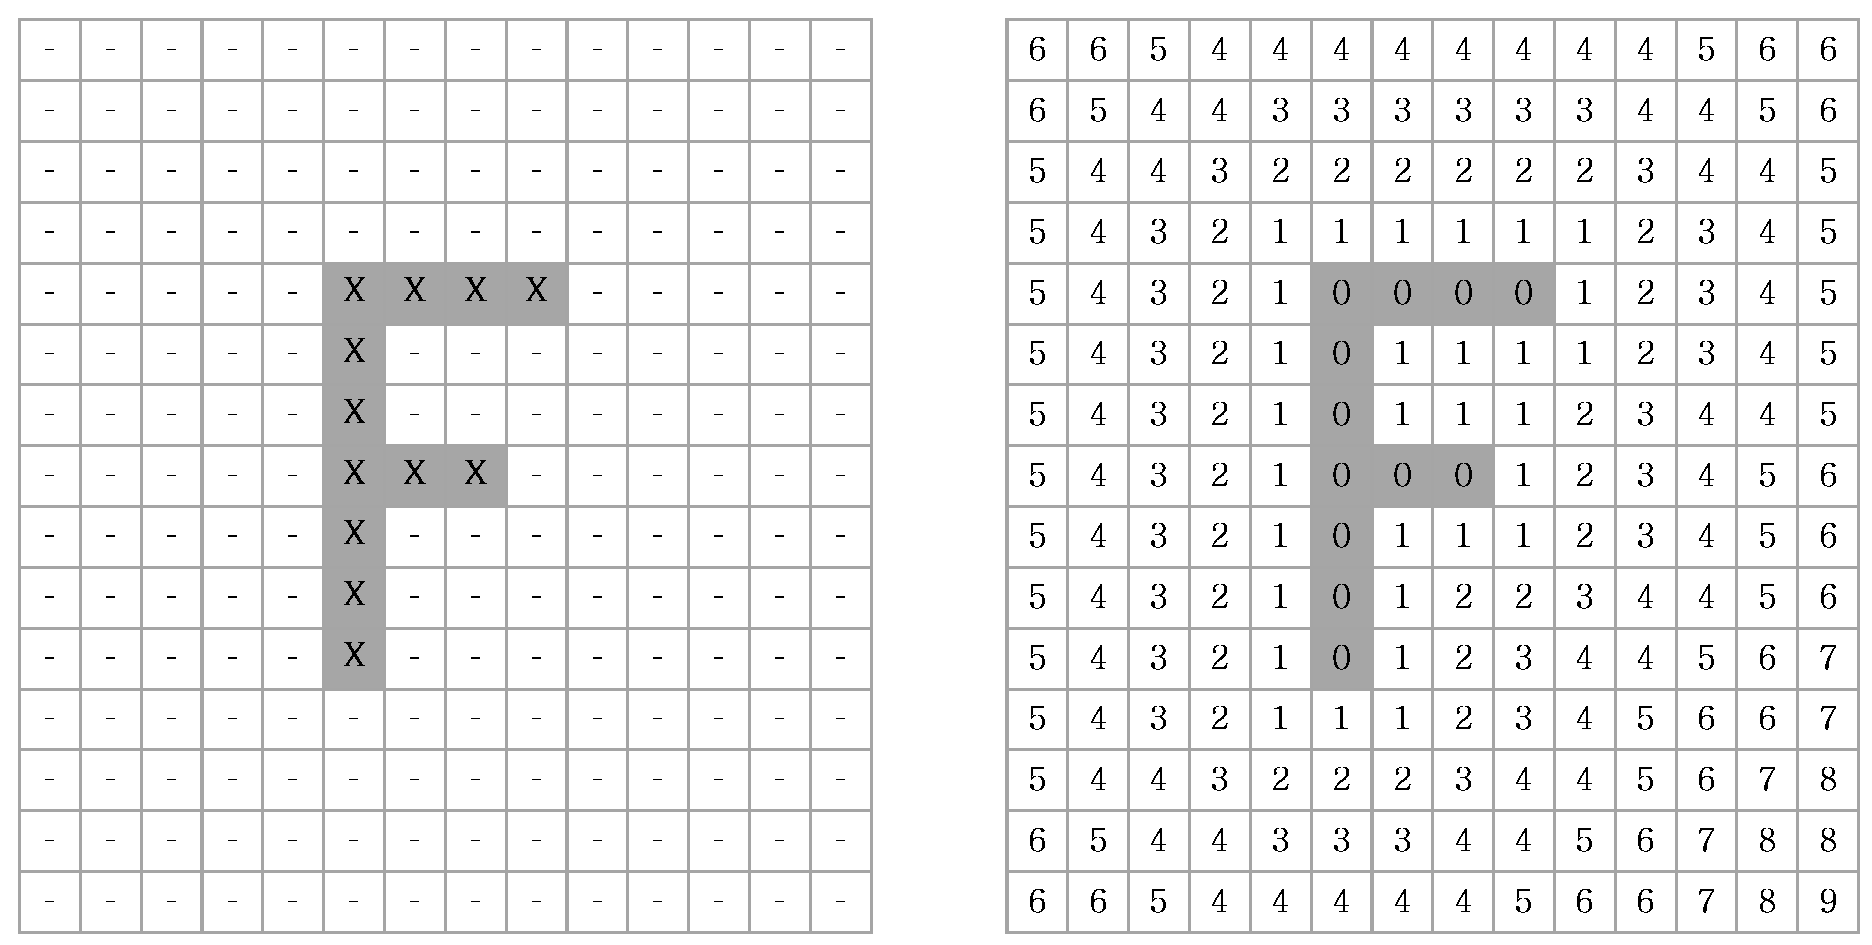
\includegraphics[width = \textwidth]{Graphics/Fundamentals/dst_tf}
    \caption[Illustration of Distance Transform]{Illustration of distance transform operation. Grid on left show the binary input image with feature pixels represented as `x' and non-feature pixels as `-'. Grid on the right corresponds to real-valued distance transformed ouput that encodes distances (Euclidean - in this case) of every non-feature pixel to its nearest feature pixel.}
	\label{fig: disttrnsf} 
\end{figure}






     
% !TeX root = ../thesis.tex

\chapter{Related Work}
\label{sec:related-work}

The presented work is inspired by multiple research fields. This chapter provides a brief overview on literature for these topics.


\section{Semantic Segmentation}

Semantic segmentation has widespread applications in medicine, industry as well as in mobile systems for semantic scene segregation. Semantic segmentation is a task of assigning class label to each pixel in a target image. Figure \ref{fig:rgb_semseg} shows an RGB image from Cityscapes dataset \cite{Cordts2015} and corresponding semantic segmentation output. Traditionally, semantic segmentation approaches relied on low-level cues like gradients, contours, contrasts and pixel relationships. Some of the successful earlier segmentation approaches are \textit{semantic texton forests} that applied decision tree ensembles at pixel level. Such random forest  based algorithm were usually coupled with noise reduction unary terms  \cite{Shotton2008}, \cite{Sturgess2009}. Significant improvements have been made in past decade since the deep learning methods were adopted for semantic segmentation task. One of the earlier approaches include \cite{Ciresan2012}, that tackled the problem of semantic segmentation of neuron membrane in electron microscopy images.


\begin{figure}[!htb]
    \subfigure[ RGB Image]{
        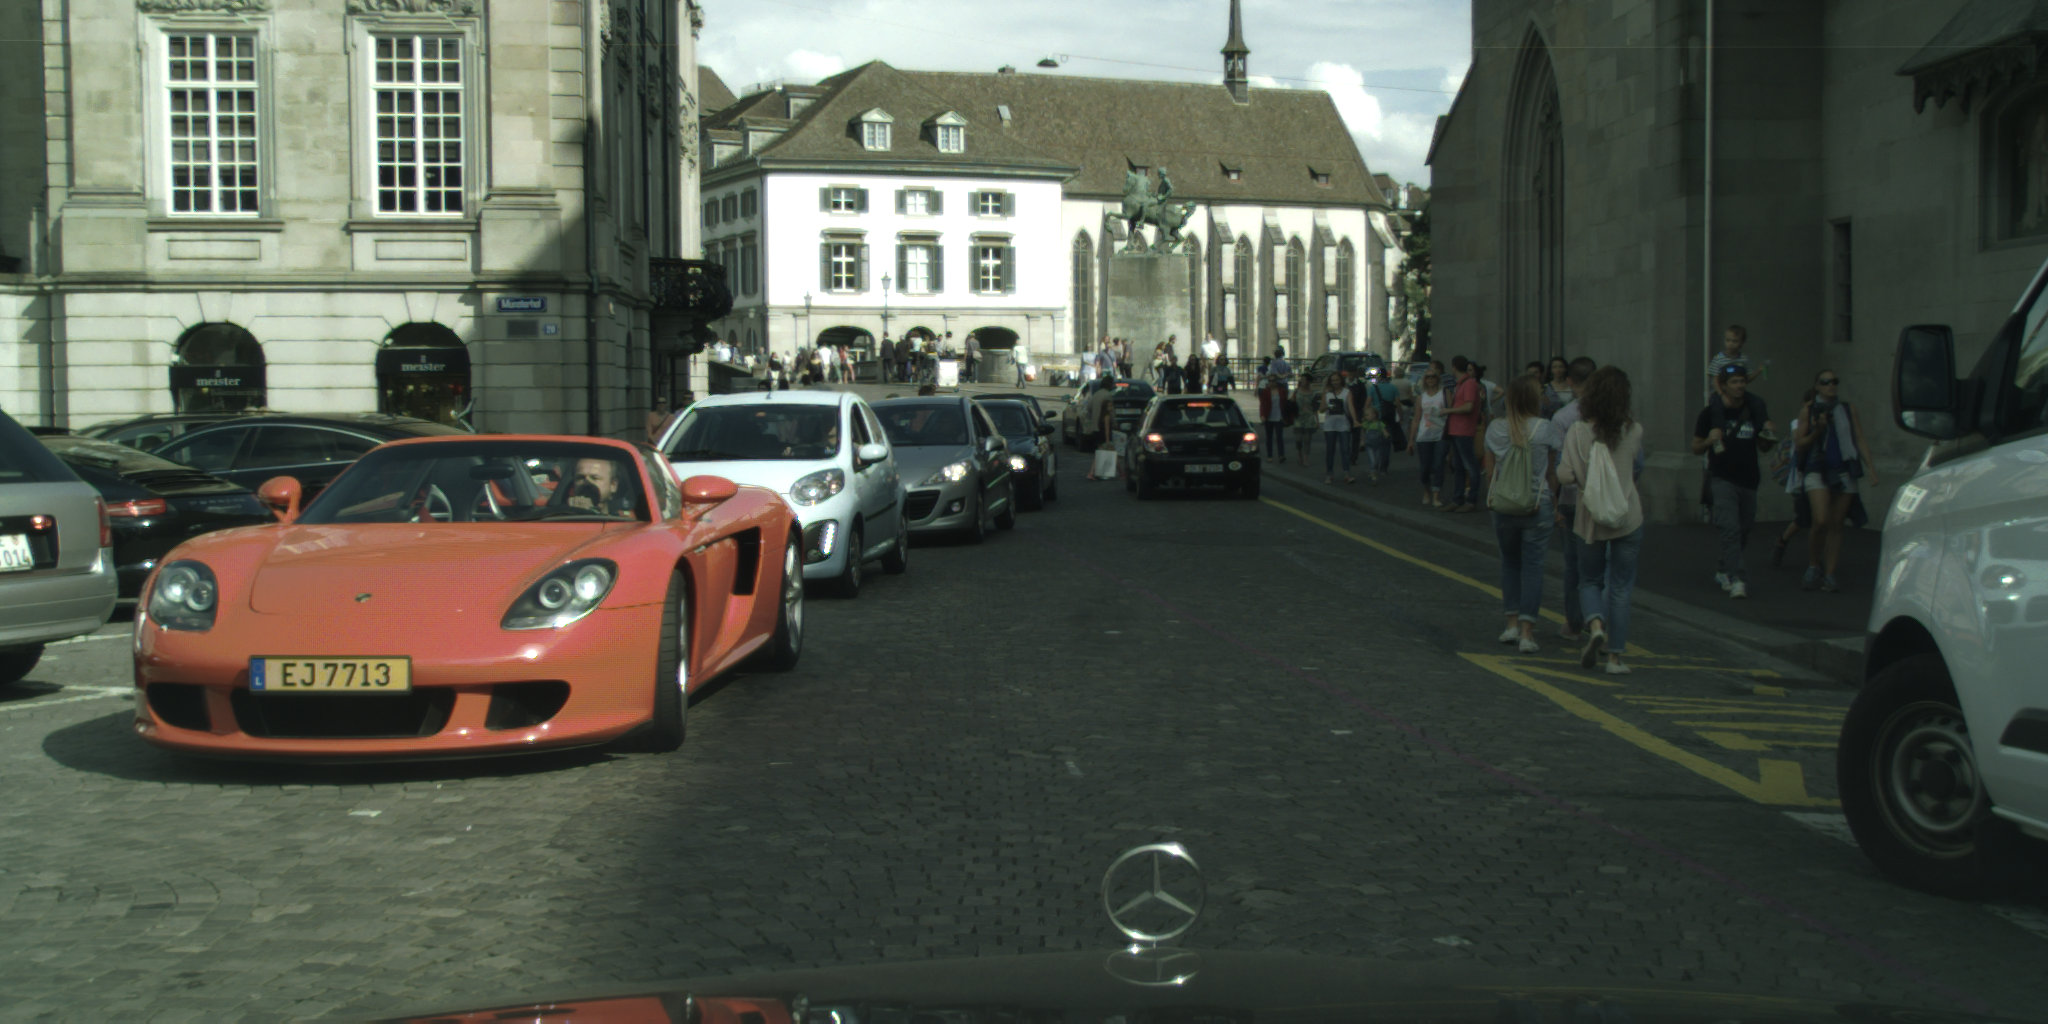
\includegraphics[width = \textwidth / 2 ]{Graphics/Related_Work/zurich_000068_000019_leftImg8bit}
        \label{fig:rgb_image}}
    \subfigure[Semantic Segmentation]{
        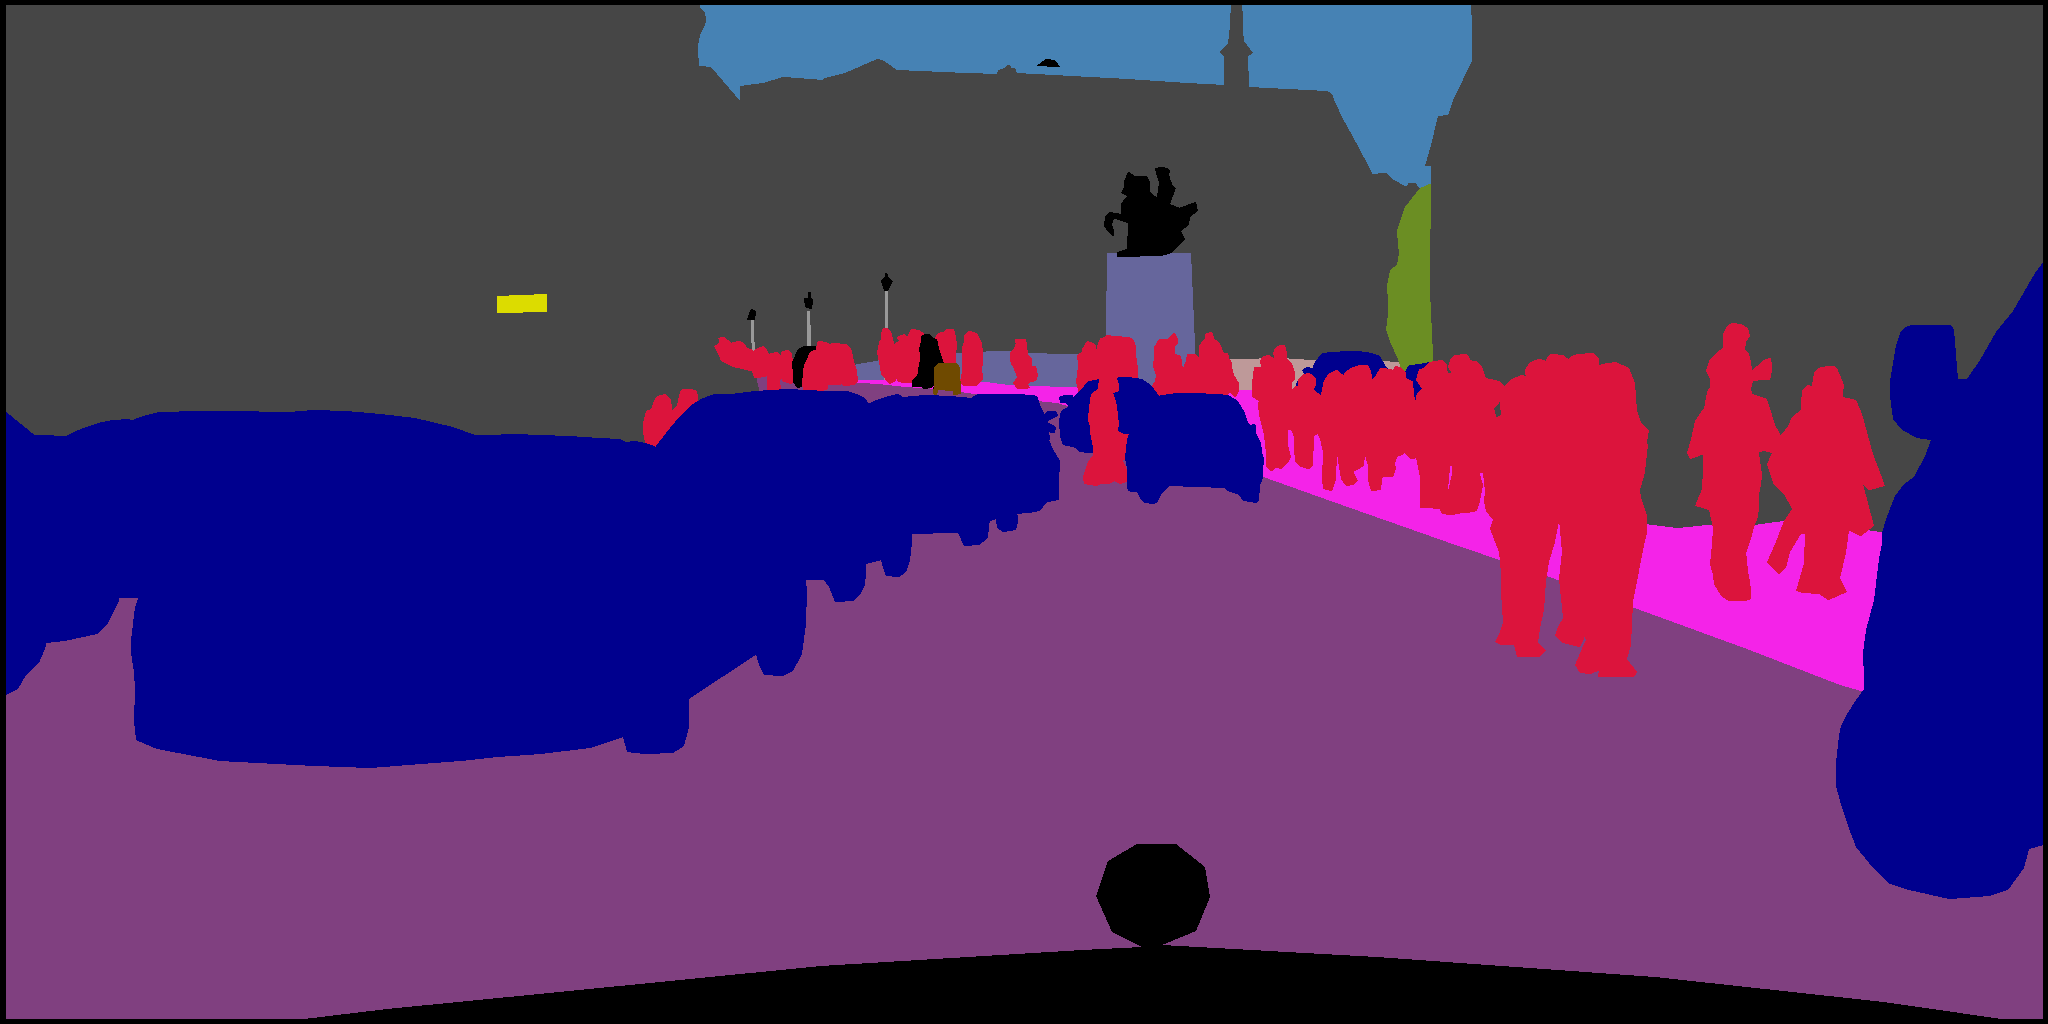
\includegraphics[width = \textwidth / 2 ]{Graphics/Related_Work/zurich_000068_000019_gtFine_color}
        \label{fig:semseggtfine}}
    \caption[RGB Image and Semantic Segmentation]{Illustration of an RGB Image taken from drivers perspective and its corresponding semantic segmentation taken from Cityscapes Dataset a) RGB Image b) semantic segmentation \cite{Cordts2015}}
    \label{fig:rgb_semseg}
\end{figure}

Recurrent neural networkss (RNNs) were used to capturing long range pixel dependencies in images for semantic segmentation. Although, it outperformed traditional methods however, boundaries were not preserved \cite{Pinheiro2014}. Significant improvements were made using end-to-end trained, fully convolutional networks (FCN), that relied on transpose convolutional layer to cop with sparse predictions and boundry preservance as faced by earlier approaches \cite{Long2015}. A similar FCN based approach was proposed that used deconvolutional layers to gradually regenerate the original resolution while maintaining boundries \cite{Noh2015}. 
 
 Since then, a huge number of publications relied on FCN architectures to solve the problem of pixel-wise semantic segmentation. Improvement in various areas of semantic segmentation were made to tweak and enhance performance in various aspects. DeepLab, used a combination of a FCN with upsampled convolutions and fully connected conditional random fields (CRFs) to improve localization performance in semantic segmentation tasks \cite{Chen2018}. They also show that atrous convolutions as explained in chapter \ref{sec:fundamentals} are helpful in explicitly controlling the field of view of convolutional filters.
 CRFs are however a post-processing step which was replaced with an encoder-decoder structure, where low-level features from lower layers were fed into higher-level layers to re-generate better boundaries \cite{Deeplabv3+:journals/corr/abs-1802-02611}. Other successful encoder-decoder structure based semantic segmentation approache was U-Net \cite{Ronneberger2015}. A later improved version is Unet++, where the encoder and decoder sub-networks are connected through a series of nested, dense skip pathways \cite{Zhou2018}.

\section{Instance Segmentation}
Instance segmentation is one of the most challenging tasks in computer vision, since it requires segmentation of all individual instances of predefined set of classes. Instance segmentation essentially requires solving object detection and semantic segmentation task simultaneously because it is desired to predict the right class label for pixels and also extent of each instance by masking it. Difference between semantic segmentation and instance segmentation has been illustrated in the figure \ref{fig:rgb_instsemseg}.

Earlier instance segmentation methods like \textit{simultaneous detection and segmentation} (SDS) \cite{Hariharan2014}, used a bottom up region proposal based approaches to score proposed regions with class labels to produce instance segmentation results. Those region proposals relied mostly on \textit{selective search} \cite{Uijlings2013} or  \textit{multi-scale combinatorial grouping} (MCG) \cite{Arbelaez2014} that extract possible coherent regions and groups them to generate multi-scale region proposals. These class agnostic proposals were scored using of \textit{Regional - Convolutional Neural Networks} (R-CNNs) based object detection algorithms \cite{Girshick2014} and its successor \textit{Fast- RCNN} \cite{Girshick2015}. Fast R-CNN is an improved verion of vanilla R-CNN that removed redundant computations by adding \textit{region of interest pooling} (RoI) pooling module. These simple region proposal methods were later replaced by more accurate neural networks based region proposals in \textit{DeepMask} \cite{Pinheiro2015}. In contrast to the DeepMask method for segmenting instances \cite{Dai2016} exploits image local coherence for estimating instances. These segment proposal networks however, were not end-to-end trainable.  First end-to-end trainable model \textit{Multi-task Network Cascades} (MNC) was proposed by \cite{Dai2016b}, that shared convolutional features and used bounding box detection to regress instance mask. MNC shares convolutional features however each sub-task was dependent on the output of from preceding branch, resulting in a complex training process and network architecture. 
FCIS was therefore first fully convolutional end-to-end trainable architecture for instance segmentation that relied on positive sensitive inside-outside score maps and was able to share features between sub-tasks  \cite{Li2017}. 

Earlier explained category-agnostic segment proposals were a bottleneck in terms of running time and were later replaced by \textit{region proposal networks} (RPN) to increase inference time. An RPN is a fully convolutional network that simultaneously predicts object bounds and objectness scores in \textit{Faster R-CNN} \cite{Ren2017}.

State of the art for instance segmentation architecture is Mask R-CNN that extends Faster- RCNN by adding a parallel branch for predicting an object mask along with branch for bounding box recognition. Structurally, Mask R-CNN is an extension of Faster- RCNN \cite{Ren2017} with an additional masking modules that segment objects inside detected bounding box. Fore more details on Mask R-CNN based instance segmentation, reader is refereed to \cite{He2017}.

\begin{figure}[!ht]
    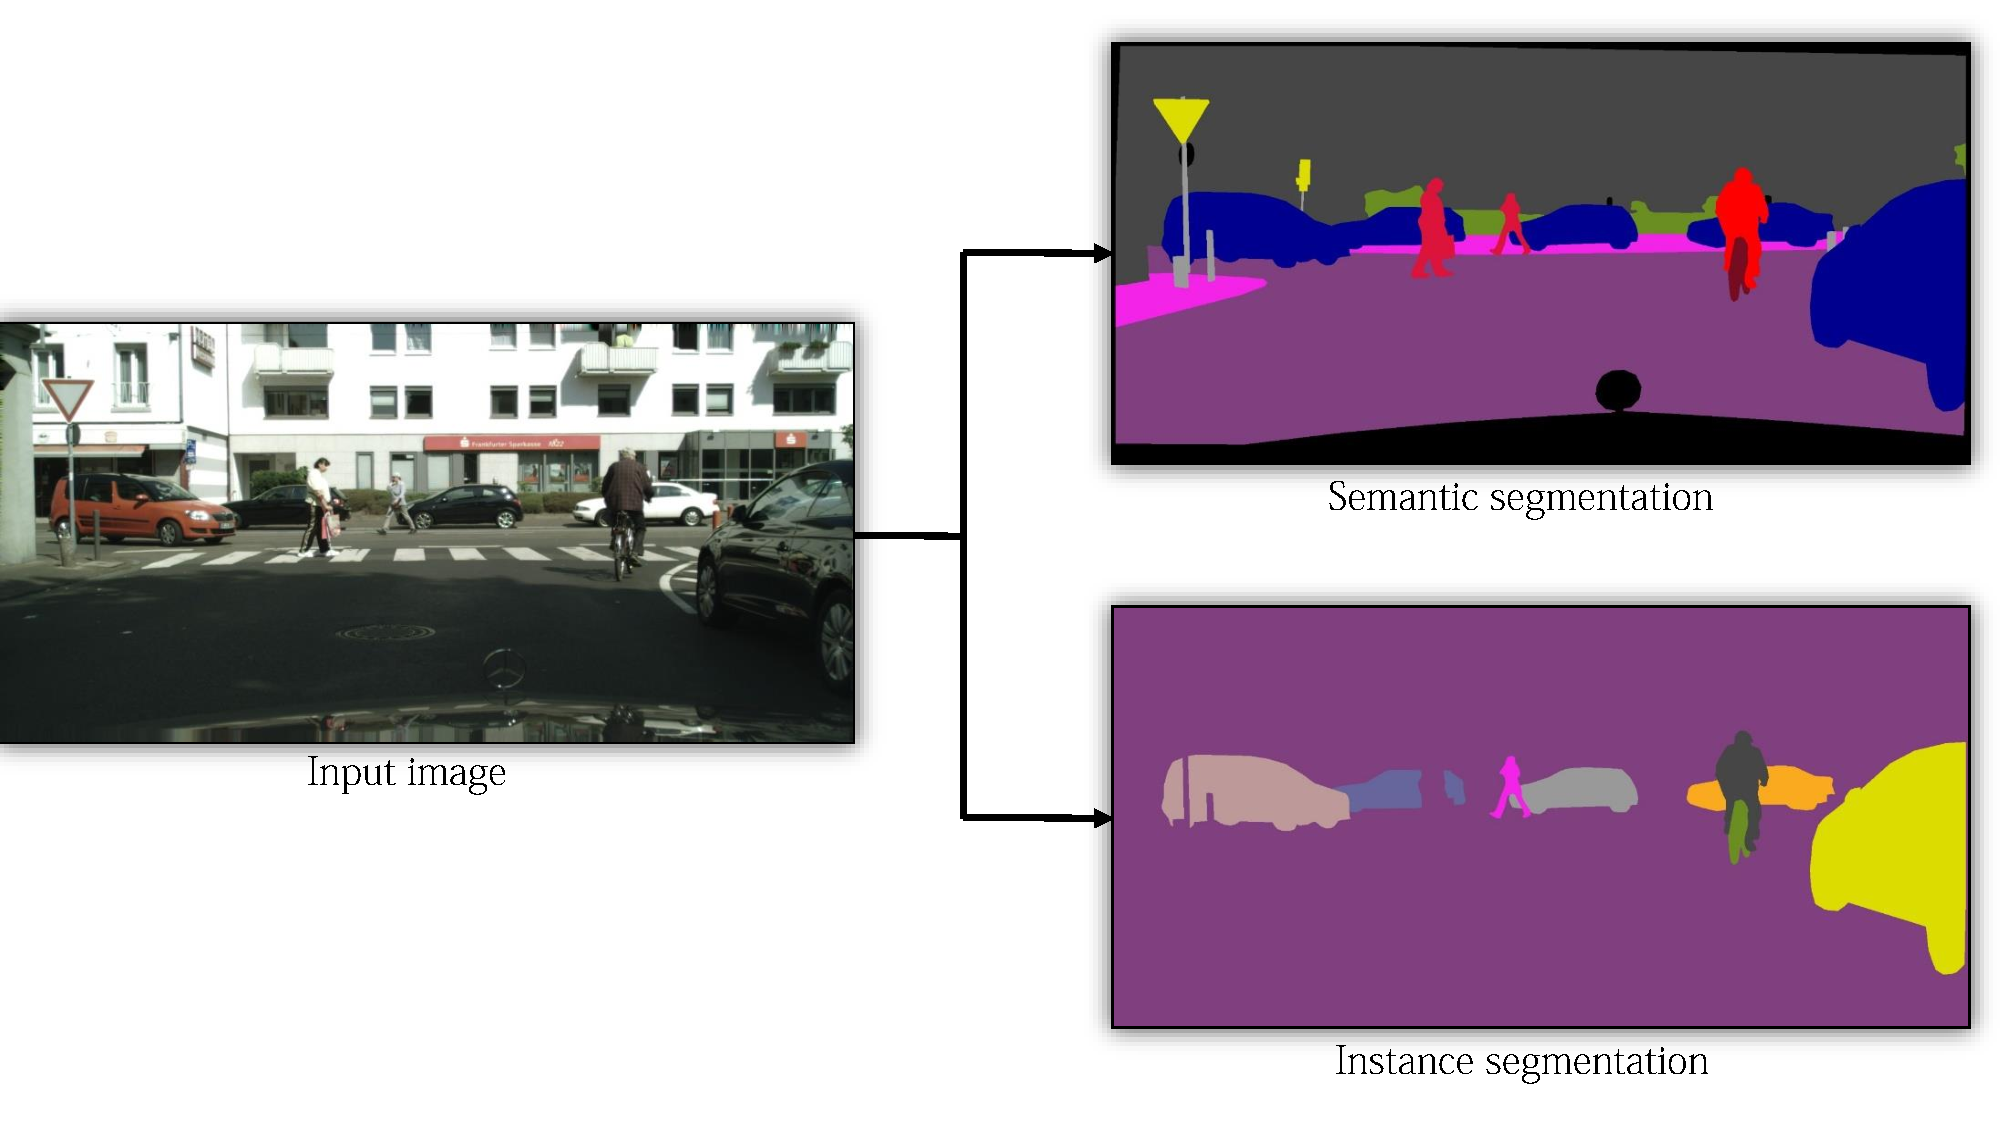
\includegraphics[width = \textwidth]{Graphics/Related_Work/SemInstImage.pdf}
    \caption[Semantic vs Instance Segmentation]{Illustration of an RGB Image taken from drivers perspective and its corresponding instance and semantic segmentation taken from Cityscapes Dataset \cite{Cordts2015}}
    \label{fig:rgb_instsemseg}
\end{figure}

\section{Panoptic Segmentation}

Panoptic segmentation aims to combine both of segmentation approaches described in former sections of this chapter. Very recently proposed panoptic segmentation task unifies the typically disjoint tasks of assigning class label to every pixel (\textit{semantic segmentation}) and detect and segment each object instance (\textit{instance segmentation}) \cite{Kirillov2019}, see figure \ref{fig:panoptic_seg} for reference.

\begin{figure}[!ht]
    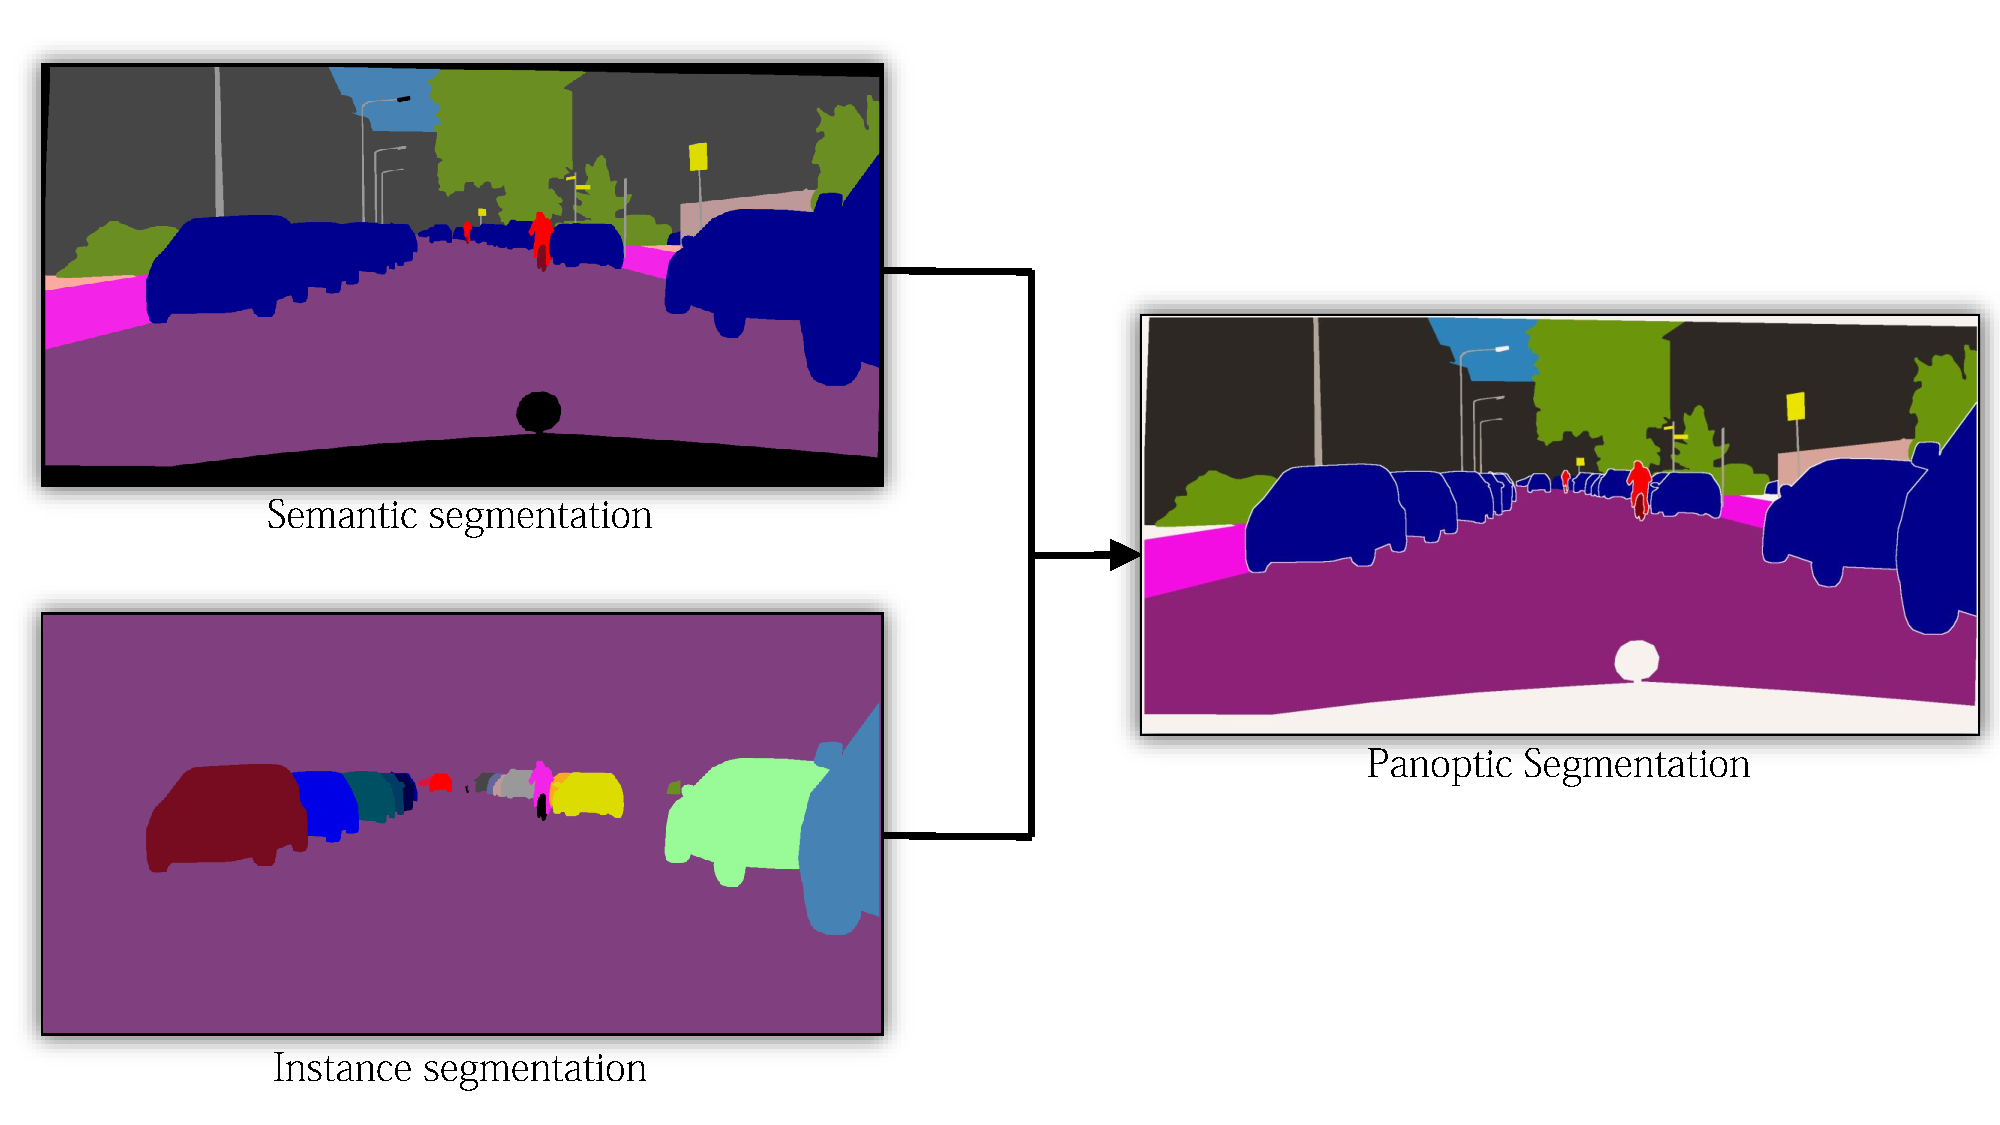
\includegraphics[width = \textwidth]{Graphics/Related_Work/PanopticSeg.pdf}
    \caption[Panoptic Segmentation]{Illustration of panoptic segmentation as a unified segmentation task -sample image taken from Cityscapes Dataset \cite{Cordts2015}}
    \label{fig:panoptic_seg}
\end{figure}


Numerous methods have been proposed for independent sub-tasks of panoptic segmentation, some of which have been briefly covered in the previous sections. However, there have been very few approaches that have tackled the task in a combined fashion. This section is dedicated to related literature review of state-of-the-art approaches that have been introduced for panoptic segmentation exclusively. 

Methods that address panoptic segmentation can be broadly classified into two
categories: 
\begin{itemize}
    \item Top-down or proposal based methods
    \item Bottom-up or proposal free methods
\end{itemize}


\subsection{Top-down approaches}

Most of the current state-of-the-art methods are top-down approaches. Panoptic segmentation task was proposed by \cite{Kirillov2019}, along with reviving the unified segmentation task, they also proposed a top-down baseline model based on PSPNet \cite{Zhao2017} and Mask R-CNN \cite{He2017}, for semantic segmentation and instance segmentation respectively. Joint training with a shared backbone that incorporates a Mask R-CNN type of architecture for instance segmentation, and augments a pyramid pooling module for semantic segmentation has been proposed by \cite{DBLPDaandeGues:journals/corr/abs-1809-02110}. An attention guided unified network that used proposal attention and mask attention module was proposed by \cite{Li2019} for joint segmentation task.
\textit{Unified Panoptic Segmentation Network} (UPSNet) introduces parameter free panoptic head to resolve conflicting and overlapping instances by prediciting an extra class. Subsequently, AdaptIS uses points to generate class agnostic instance masks and combines with semantic segmentation pipeline to perform panoptic segmentation \cite{adaptis2019}. More recently, \cite{Porzi2019} proposed an architecture that leverages novel segmentation head to integrates multi-scale features generated by a feature pyramid network (FPN) \cite{Lin2017} and conveyed using Deeplab-like \cite{Chen2018} module. 


Finally, \textit{Efficient panoptic segmentation architecture} (EfficientPS) is the current state-of-the-art at the time of writing this thesis \cite{mohan2020efficientps}. EfficientPS consists of a shared backbone that encodes and fuses multi-scale features. They propose a new semantic
head that aggregates features and propose a variant of Mask R-CNN as the instance head along-with a panoptic fusion module that integrates the output logits from both the heads to generate final panoptic output.

\subsection{Bottom-up approaches}

There have been very few bottom up, proposal free methods for panoptic segmentation. First bottom-up panoptic segmentation was \textit{Deeper-Lab}, that adopted bounding box corners as well as object center points for class-agnostic instance segmentation \cite{DBLPDeeperLab:journals/corr/abs-1902-05093}. Recently, \cite{Gao2019} proposed pixel grouping based on pixel-pair affinity pyramid \cite{Liu2018} with an efficient graph partition method \cite{Keuper2015}. Subsequently, \textit{panoptic-deeplab} was proposed as a solid baseline for bottom-up methods \cite{Cheng_2020_CVPR}. Panoptic-deeplab adopts the dual-\Gls{aspp} and dual-decoder structures specific to semantic and instance segmentation respectively. Semantic segmentation branch relies on typical design of deeplab \cite{Chen2018}, while instance segmentation branch adopts a simple instance center regression approach to generate class-agnostic instance masks. These instance masks are combined with semantic segmentation to generate panpotic segmentation. Presented work is majorly inspired by aforementioned proposal-free, bottom up panoptic segmentation architecture.   		
% !TeX root = ../thesis.tex

\chapter{Data Representation}
\label{sec:data_representation}

This chapter presents description about data representations. Since panoptic task requires to learn both modalities i.e. semantic segmentation and instance segmentation, it also demands the ground-truth label data to be presented in a suitable format for either modalities. First section of this chapter discusses semantic ground-truth representation and dataset used for this purpose. Second section is dedicated to the description of various instance representations and encodings that are conceived and generated during the course of this master thesis.  




\section{Semantic Label Representation}

This section describes about the dataset used for experiments, more specifically this section gives a brief overview of semantic segmentation labels used for this purpose. 

\paragraph{Cityscapes}

Cityscapes is a large-scale benchmark dataset that contains diverse street scenes from 50 different cities, with a high quality pixel-level and instance-level semantic labeling annotations of 5000 frames at resolution of $1024 \times 2048$ in addition to a larger set of 20000 coarsely annotated frames \cite{Cordts2015}. Cityscapes has become a default benchmark for semantic segmentation due to its high quality of annotation along with high resolution labeled images \cite{DBLPbenchmark:journals/corr/abs-1709-07322}. Figure \ref{fig:cityscapes} illustrates
some example segmentation annotations from cityscapes dataset overlaid on corresponding RGB image captured in different cities. Furthermore, fine-annotations are further divided into 3 splits, which is an important step carried out for learning process. One split is used for learning the parameters in an iterative process, while other is used for monitoring models performance during  the training (learning process), the last split is used at the end of learning process to test models performance.

\begin{table}[!htbp]
    \centering
        \begin{tabular}{llll}
        \hline \bigskip & \multicolumn{3}{c} {Cityscapes } \\
        \cline { 2 - 4 } Dataset split & $\mathrm{CS}_{\text {train }}$ & $\mathrm{CS}_{\text {val }}$ & $\mathrm{CS}_{\text {test }}$ \\
        \hline Number of images  & 2975 & 500 & 1500 \\
        \hline
        \end{tabular}
    \caption[Data Splits in Cityscapes]{Training, validation and test splits of Cityscapes.}
    \label{tab:cityscapessplits}
\end{table}



\begin{figure}[!ht]
        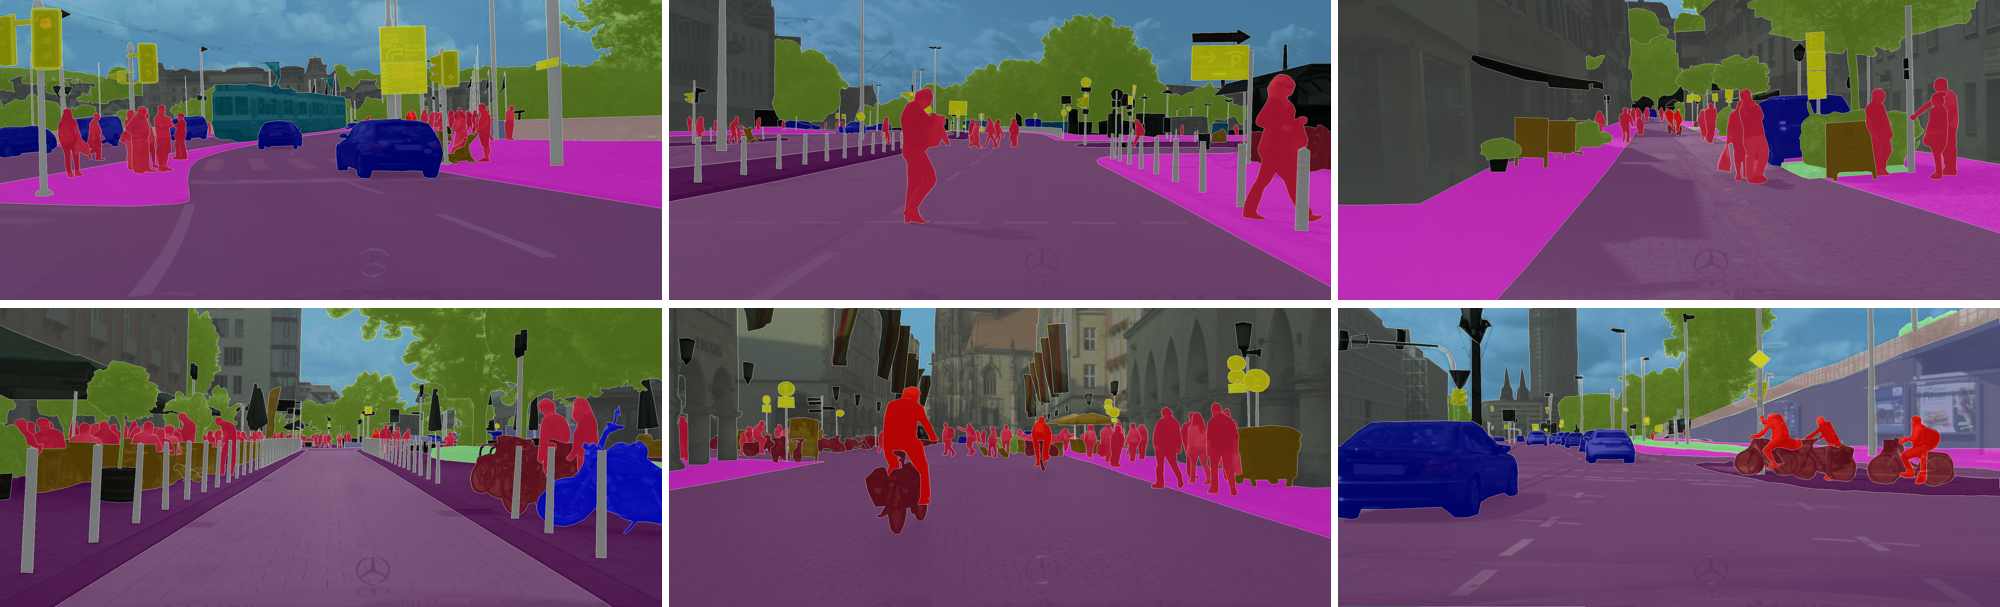
\includegraphics[width = \textwidth]{Graphics/Data_Representation/cityscapessamples.png}
    \caption[Examples from Cityscapes dataset]{Illustration of sample images overlayed with corresponding semantic annotations taken from cityscapes dataset \cite{Cordts2015}}
    \label{fig:cityscapes}
\end{figure}


\newpage
\begin{itemize}
    \item \textbf{Train} - split used to train model for optimizing parameters
    \item \textbf{Validation} - split used to monitor model performance during learning
    \item \textbf{Test} - split used to evaluate performance of trained model at the end of learning process.
\end{itemize}

Training labels for semantic segmentation are used directly as provided by cityscapes. The groundtruth is annotated to distinguish 31 different classes, however they are usually summarized to 19 classes for training purposes which have also been used within the scope of this thesis as such.

\section{Instance Representation}

One core objective of the presented work is to learn pixel-level relationships for instance segmentation instead of using $2-stage$ objection detection like architecture for instance segmentation. This section is dedicated to describe the instance representations for encoding instance information which is later learned by the network in combination with semantic segmentation. The following section illustrates instance representations that are conceived during the scope of this thesis. A general approach adapted to represent pixel relationships is to encode the distance for every pixel within an instance to its corresponding center point. Firstly, the representation and encoding center point information is discussed. Subsequently, various offset representations are discussed that in some way describe the offset of every pixels from its respective center. 


\subsection{Center Points Representation}

It is desire
d to learn instance representations in addition to semantic segmentation of the scene. To generate an instance representation, center point for every instance is considered to be a reference point. Therefore it is critical that this reference representation is robust and efficiently learned by the network. To locate a center from an instance annotation, distance transform is employed to binary mask of individual instance  \cite{Borgefors1986} -  see chapter \ref{sec:fundamentals}. In addition to being robust against heavy occlusions, this also has the benefit of being a consistent approach for locating center of visible portion of instances appearing in an image. In computer vision literature, it is common to denote key points by encoding them with a 2d - gaussian distribution \cite{DBLPCPM:journals/corr/WeiRKS16}, \cite{Bulat2016HumanPE}. Center points extracted from every instance mask are therefore encoded by a probability distribution around the center. A visualisation of such center rendering and encoding each center with a 2d - gaussian like distribution has been shown in the figure \ref{fig:centerpoints} 

\begin{figure}[!ht]
    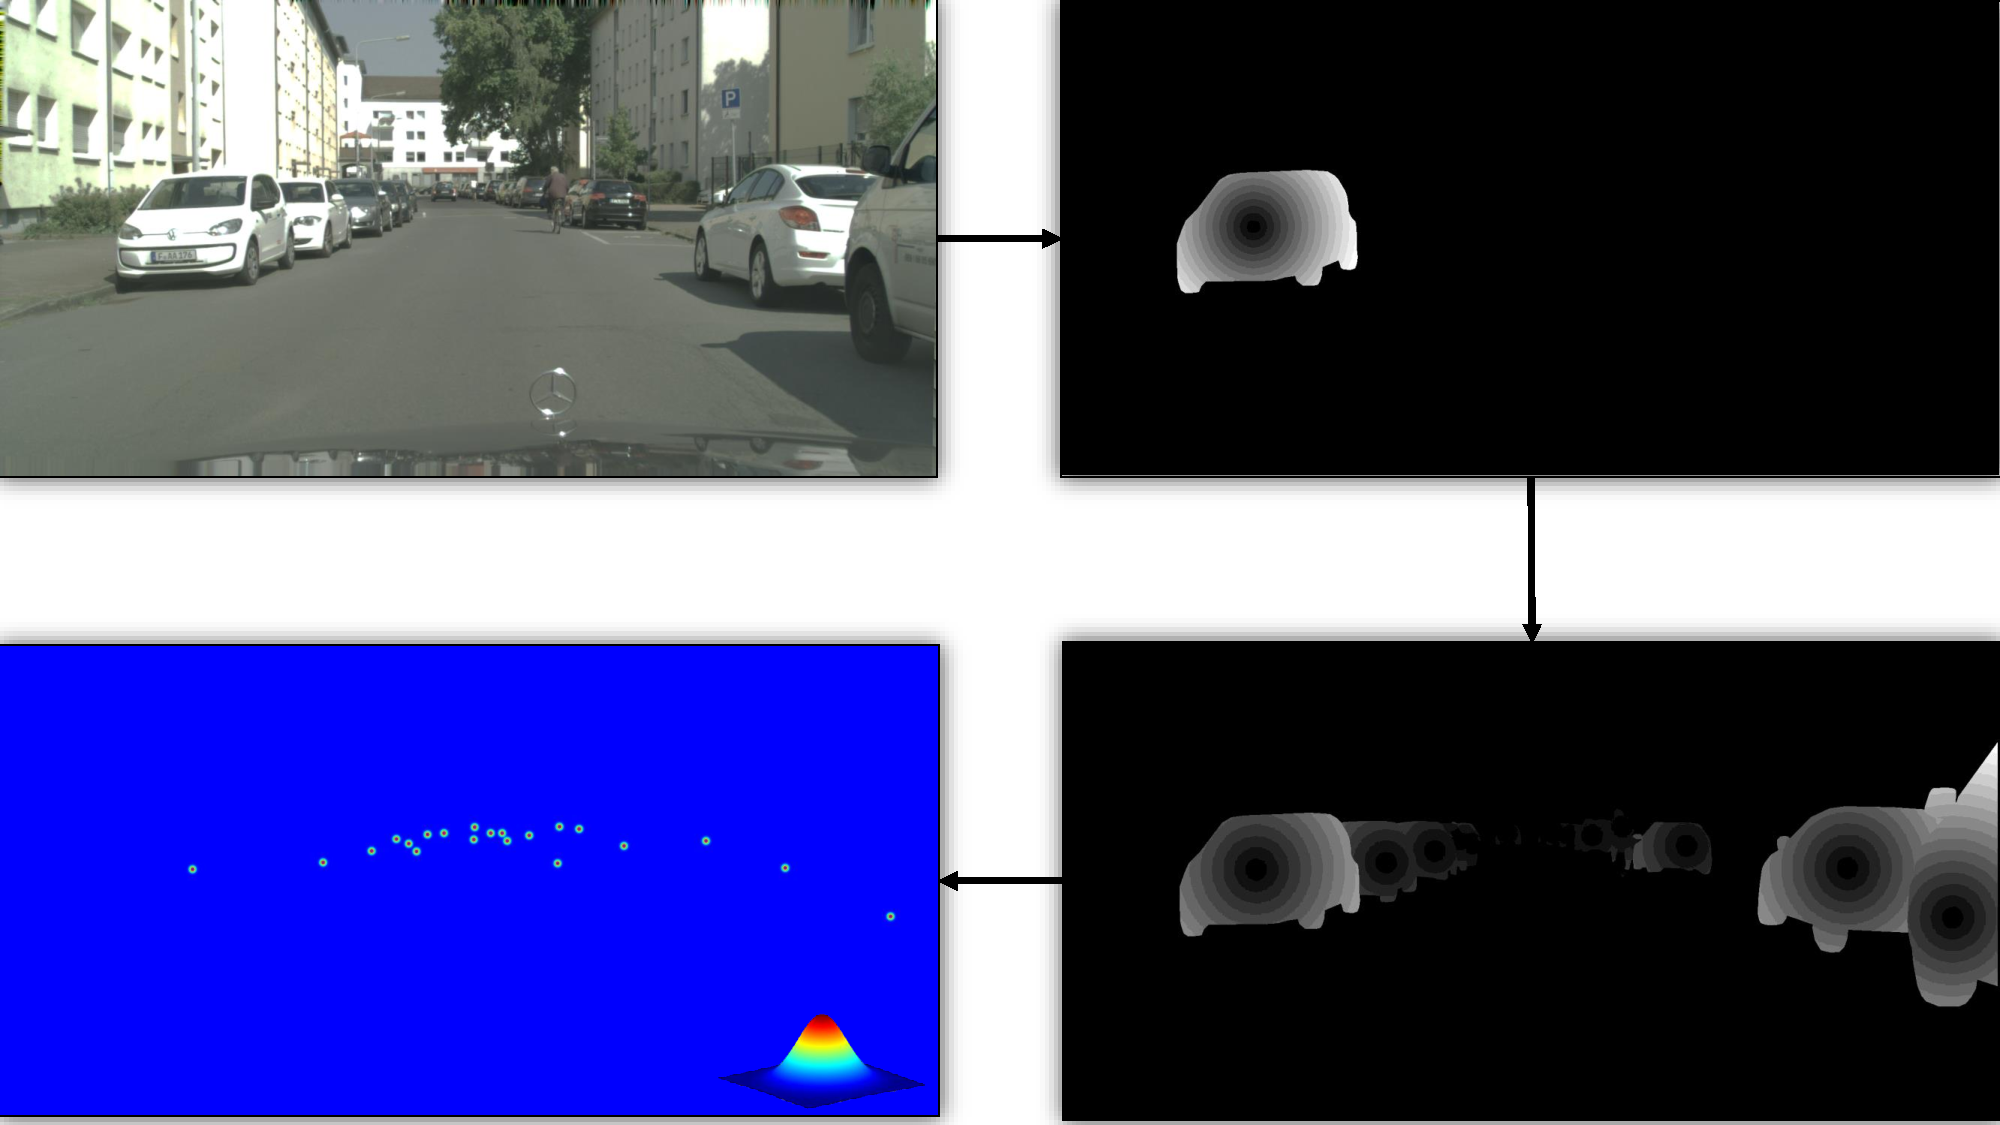
\includegraphics[width = \textwidth]{Graphics/Data_Representation/dist_centerpoints.pdf}
    \caption[Center Encoding Process]{Illustration of center encoding process. Distance transformation is applied to every instance and pixel with largest distance to the boundary is selected to be the center for each instance. Subsequently, each center point is encoded with a 2d - gaussian distribution.}
    \label{fig:centerpoints}
\end{figure}

It has also been shown that representing a key-point with a gaussian distribution comparatively improves performance, such experiments have also been carried out by \cite{Cheng_2020_CVPR}, they also show that an additional $0.8\%$ improvement can be made if such an encoding is used and optimized using L2 -loss between predicted and ground-truth label instead of categorical cross-entropy (which is a commonly employed loss function for semantic segmentation problems in image domain). 

However, the right size for this purpose is still an open question. If a center point is encoded with a probability distribution of very small standard deviation ($\sigma$) , it might not considerably influence the learning process, since every image has a high resolution of 1024 $\times$ 2048, on the other hand if the $\sigma$ is too large, it might be very dispersed around center point region (thus not representing precise location of center point) and might also pose a problem of overlapping nearby center points. Hence it is desired to generate datasets with center-points encoded as gaussians of variable standard deviations $\sigma$ and compare the performance to reason about the right distribution parameters. For this purpose, 4 datasets have been generated that encode center-points with different $\sigma$, which in this case are chosen to be 2, 4, 8 and 16, see figure \ref{fig:distsizes}. The results for which have been discussed in evaluation chapter.

\begin{figure}[!ht]
    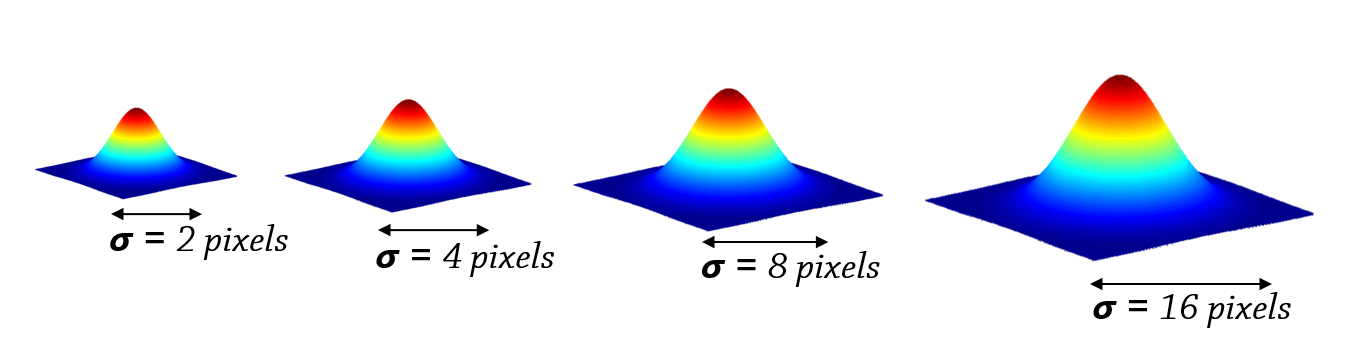
\includegraphics[width = \textwidth]{Graphics/Data_Representation/distributions}
    \caption[Different Distribution Sizes]{Visualisation of different guassian distributions with variable  standard deviations of  2, 4, 8 and 16 - from left to right respectively.}
    \label{fig:distsizes}
\end{figure}



\subsection{Offset Representation}

\label{subsec:offsets}
Another important information that has been used to encode instances is\textit{ offset vectors}. Offset vector representation can be elaborated as - a representation where every \textit{thing} class pixel encodes the distance to its corresponding center hence, the \textit{offset which when added to the pixel at given location will move it to its corresponding center.} Few such offset vector representations that have been generated and evaluated during this work are named as follows:

\begin{enumerate}

    \item End-to-end encoding
    \item Center-to-end encoding 
    \item Euclidean encoding

\end{enumerate}

Visualisation of the above mentioned offset vector encodings has been shown as rgb images in the figure \ref{fig:RGB_encodings}. These representations will be explained in detail in the following sub-sections.

\begin{figure}[!ht]
%\centering
        \subfigure[Center-to-End Encoding]{
        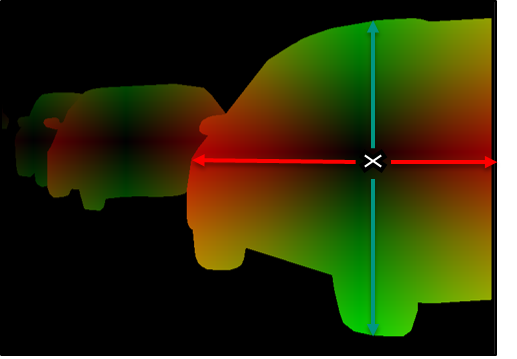
\includegraphics[width = \textwidth / 3 ]{Graphics/Data_Representation/c2e_vis_img}
        \label{fig:c2e_img_vis}}\subfigure[End-to-End Encoding]{
        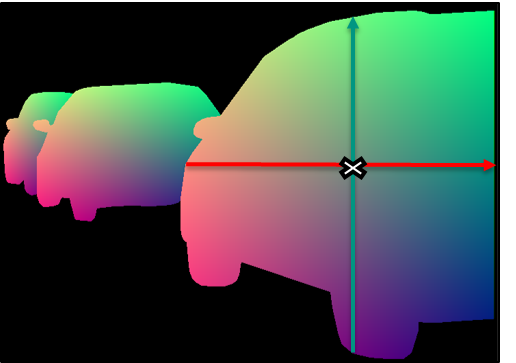
\includegraphics[width = \textwidth / 3 ]{Graphics/Data_Representation/e2e_vis_img}
        \label{fig:e2e_img_vis}}\subfigure[Euclidean Encoding]{
        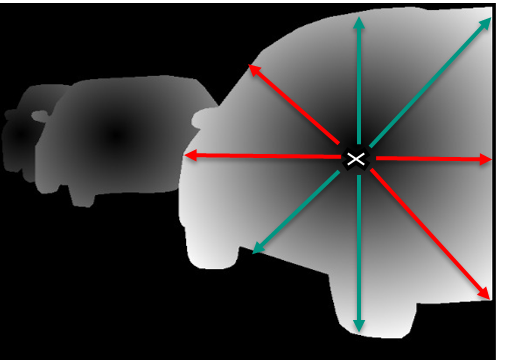
\includegraphics[width = \textwidth / 3 ]{Graphics/Data_Representation/euc_vis_img}
        \label{fig:euc_img_vis}}
        \caption[RGB Visualisation of Offset Vectors Encoding]{Visualisations of conceived encodings as rgb images a) center to end encoding b) end to end Encoding c) euclidean encoding}
        \label{fig:RGB_encodings}
\end{figure}

\subsubsection{End to End Encoding}
\label{subsec:e2e}
One way to encode aforementioned offset is by encoding both distance and direction information at given pixel location. The value encoded by each pixels exhibits a positive or a negative distance to the center point depending on it's relative position with respect to center. Additionally, the offset in horizontal axis and vertical axis are encoded independently i.e. one channel is used to record the offset in x-axis and another channel records the offset in y-axis. This can be understood by a simple case in horizontal direction, where pixels on the left side to the center will have a positive distance to the center - representing a positive offset needed to reach to the center and pixel on the right side relative to center would exhibit a negative offset - representing a negative offset needed to reach the center point.  Encoding offsets in such a way yield a near perfect representation where each pixel can be re-assigned to one of given centers at hand.  
\begin{figure}[!ht]
    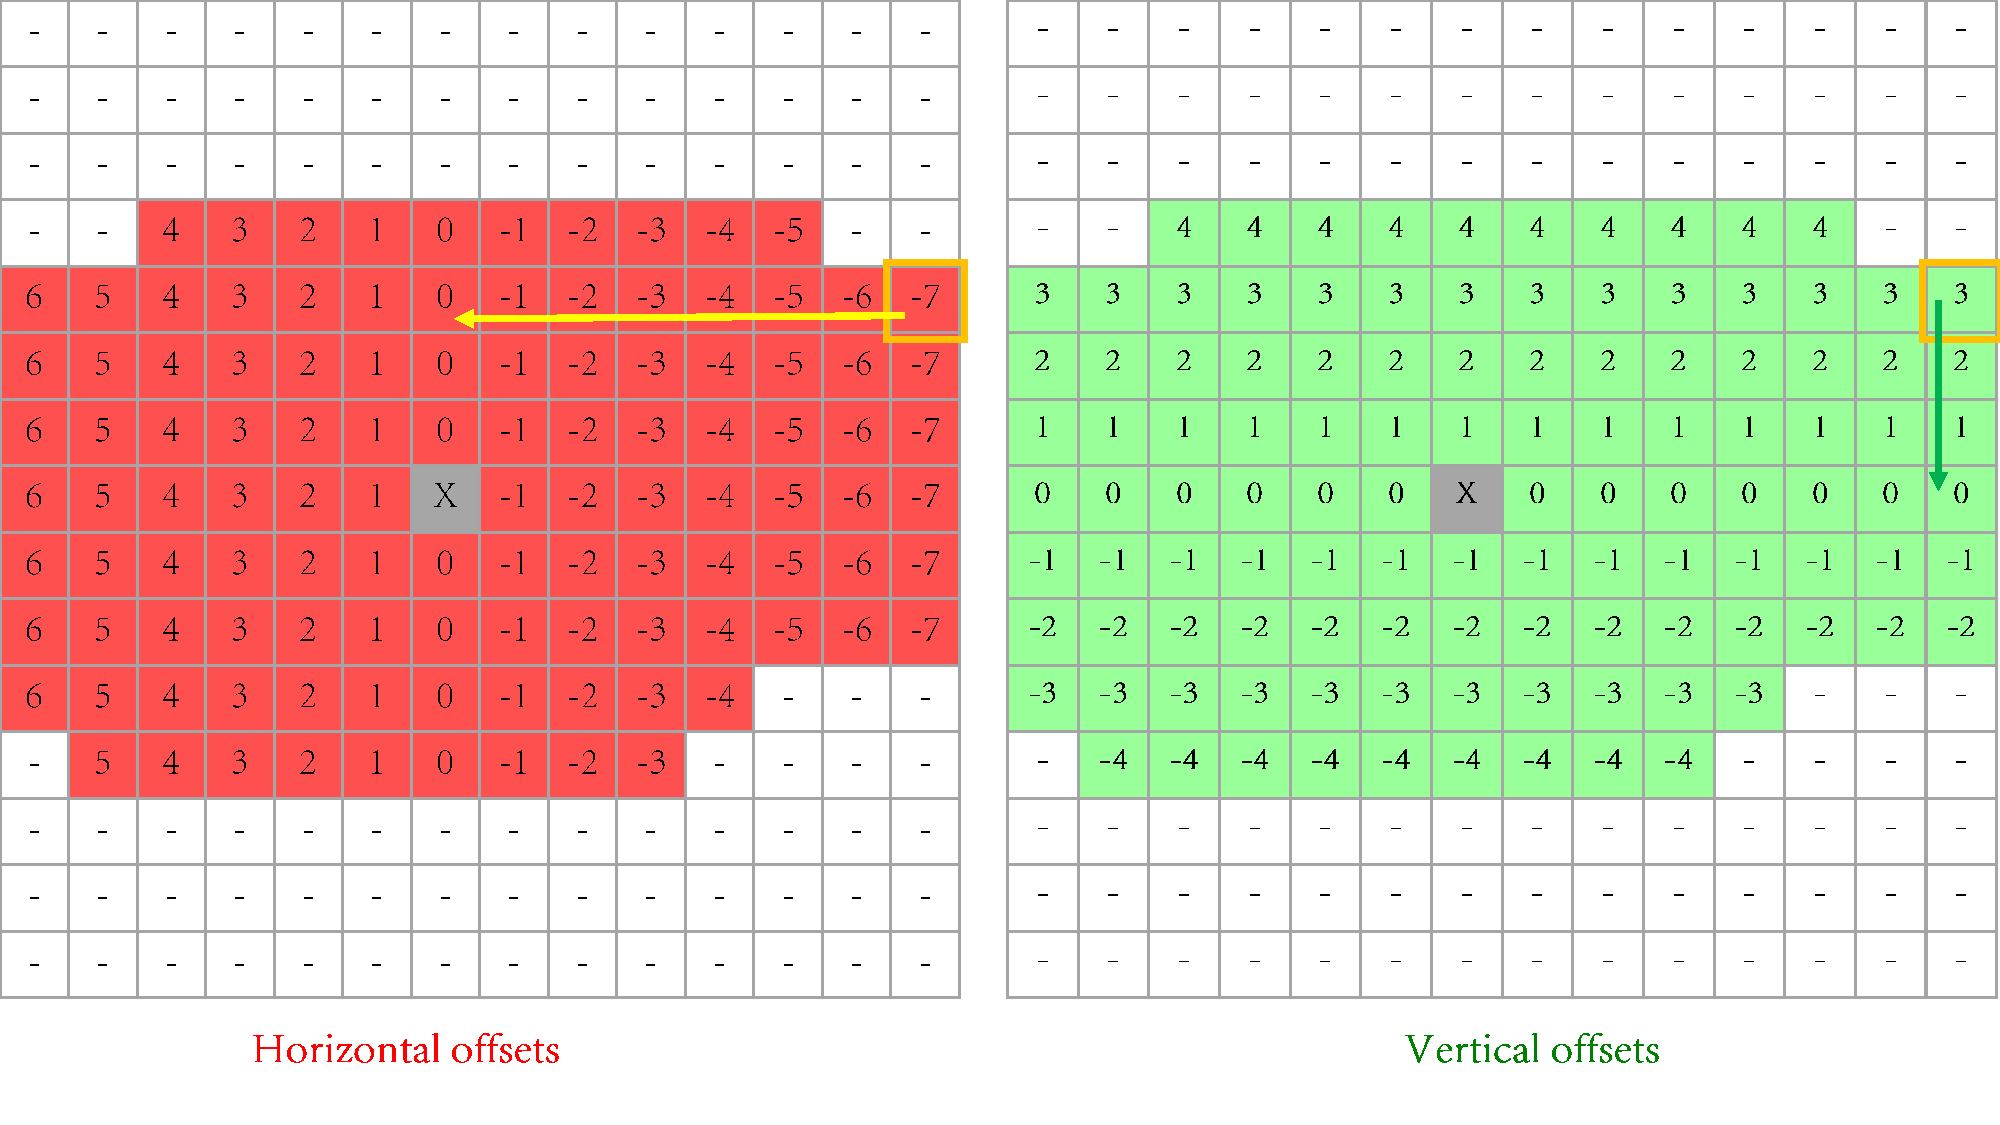
\includegraphics[width = \textwidth]{Graphics/Data_Representation/c2e_Encoding.pdf}
    \caption[Center to End Encoding]{Illustration of End-to-End encoding}
    \label{fig:e2e_vis_pixels}

\end{figure}

Once, the offset in horizontal and vertical axis $o(i, j)$ is extracted for a given pixel at location $(i, j)$, from both channels, these offsets can be added to the pixel location yielding the location of the center  $C_{k}$ of instance that pixel belongs to. Illustration of such an offset vectors representation has been shown in the figure \ref{fig:e2e_vis_pixels}. 

It can be seen from figure \ref{fig:e2e_vis_pixels}, that pixels on right side of center point are encoded as negative offsets in horizontal offset representation. Similarly, pixels below center point are encoded as negative offsets in vertical offset representation. Hence explicitly defining the direction as well as magnitude needed to reach center point. Such representation which one learned would just require a simple regression to group pixels with their corresponding centers. Another observation that can be made from this representation is the fact that offset values increase on one side of the center while decrease on the other side of the center hence a representation where offset values increase linearly between either ends of the instance. Therefore it has been named as \textit{End-to-End Encoding}. See figure \ref{fig:e2e_plt_vis} for reference.

\subsubsection{Center to End Encoding}
\label{subsec:c2e}
Another possibility to encode offset is encoding only distance information irrespective of direction towards the center at given pixel location. 

Since, direction information is not considered explicitly, it might appear as if encoding such offset representation would result in ambiguity while recovering the instances by regressing pixels to their centers. However, it can be shown that this is not the case. The offset vector therefore always exhibit positive distance to the center point irrespective of position with respect to center.  Here as well, the offsets in horizontal axis and vertical axis are encoded independently i.e. one channel is used to record the offset in x-axis and another channel records offset in y-axis. 
As, direction information is not explicitly encoded, it then requires additional post-processing step by inverting the offset values on one side in both horizontal and vertical offset representations. Theoretically, if network learns to predict as good as original groundtruth labels, it would result in a very adequate re-assignment of all the pixels to one of the centers. 

Once,  the offset vectors are inverted to re-construct offset vectors with direction information,  offset  in  horizontal  and  vertical  axis $o(i,j)$  is  extracted  for  a  given  pixel  at location $(i,j)$, from both channels, these offsets can be added to the pixel location $(i,j)$ yielding the center $C_{k}$ of instance that pixel belongs to. Illustration of such an offset vectors representation has been shown in the figure \ref{fig:c2e_vis_flip}. It can be seen the representation has taken the form of the previous end to end offset, which would then again employ a simple regression to group pixels with their corresponding centers.
Offset values appear to increase on either sides of the center point hence a representation where offset values increase monotonically on either side of center point of an instance. Therefore  it has  been named as center-to-end encoding. See figure \ref{fig:c2e_plt_vis} for reference.


\begin{figure}[!ht]
%\centering
        \subfigure[Center-to-End Encoding]{
        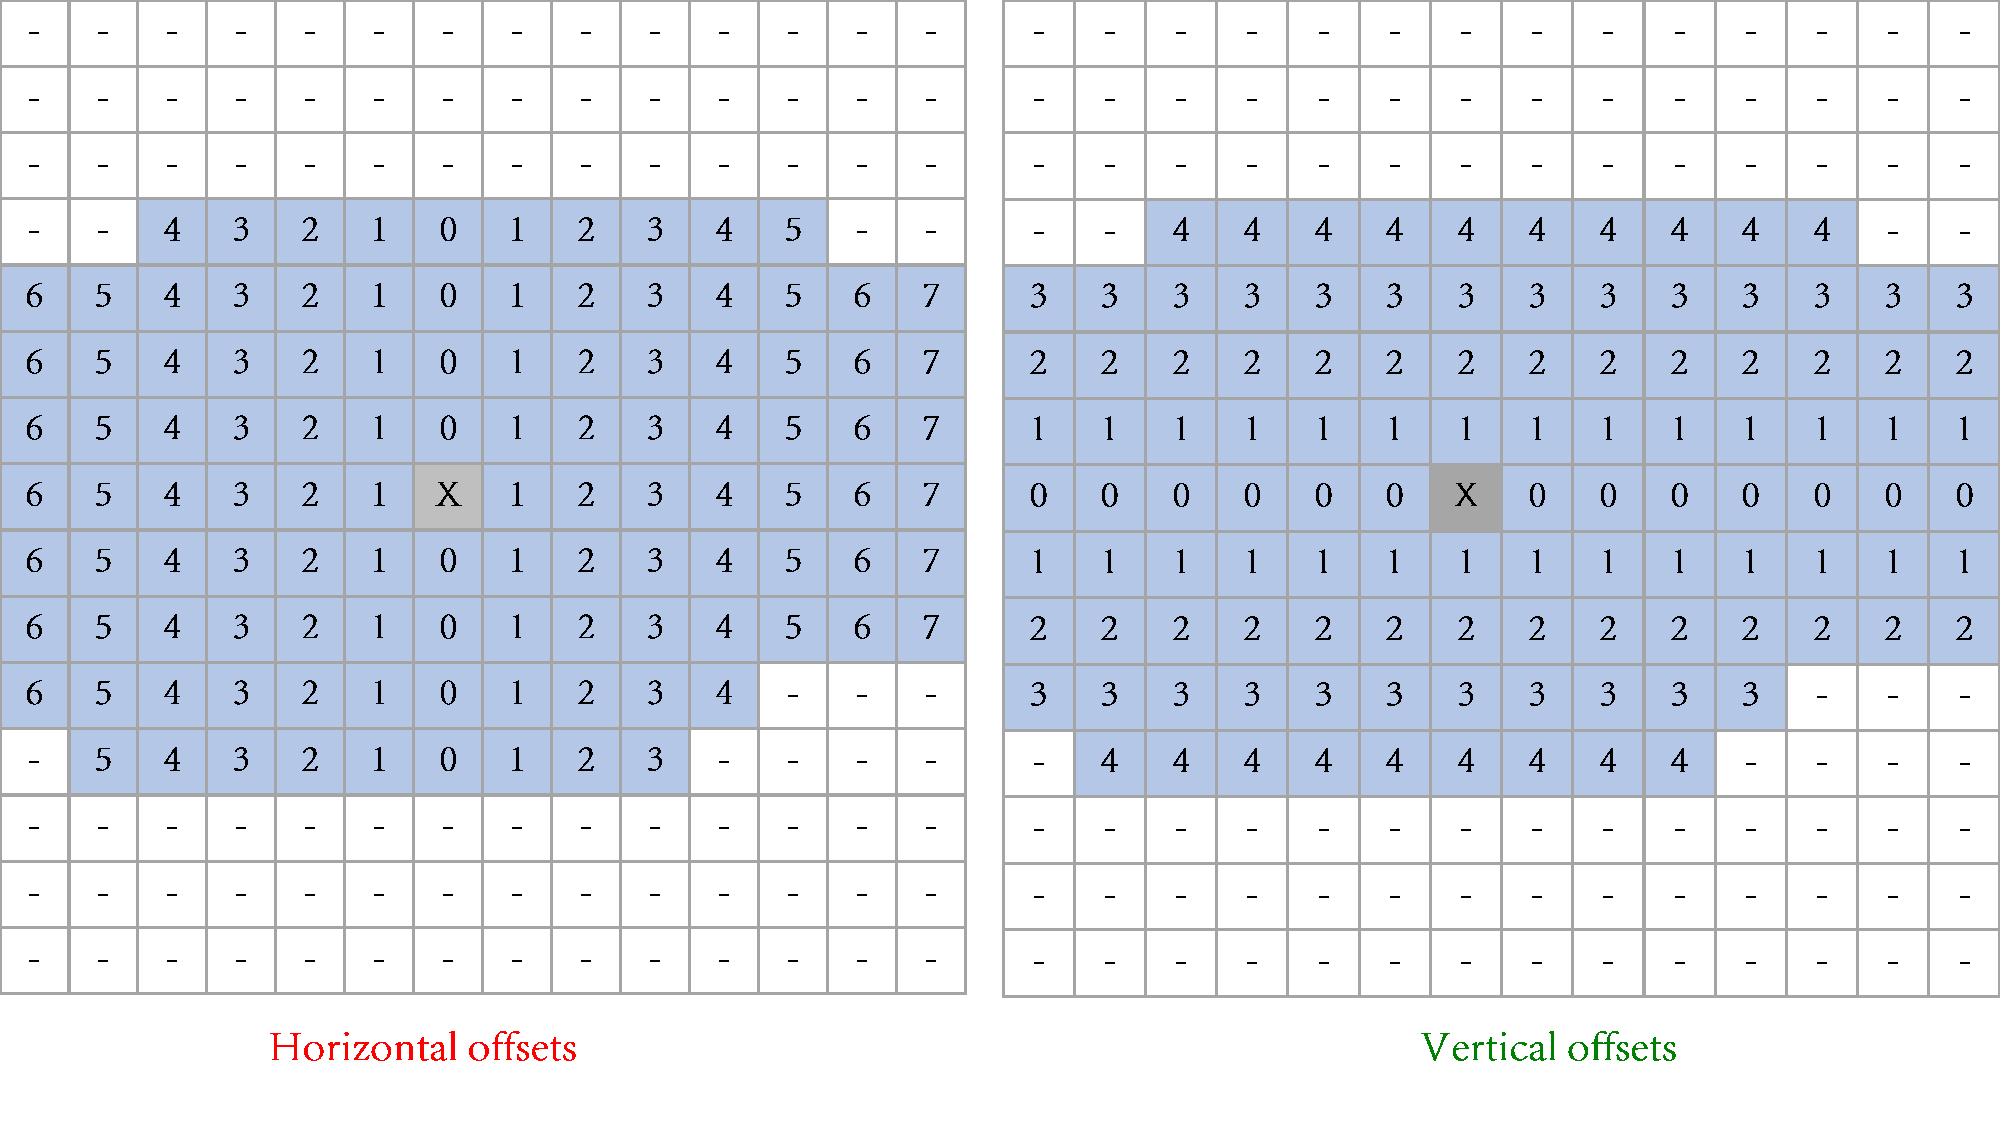
\includegraphics[width = \textwidth]{Graphics/Data_Representation/c2e_vis}
        \label{fig:c2e_vis}}
        
        \subfigure[Center-to-End Encoding Inverted]{
        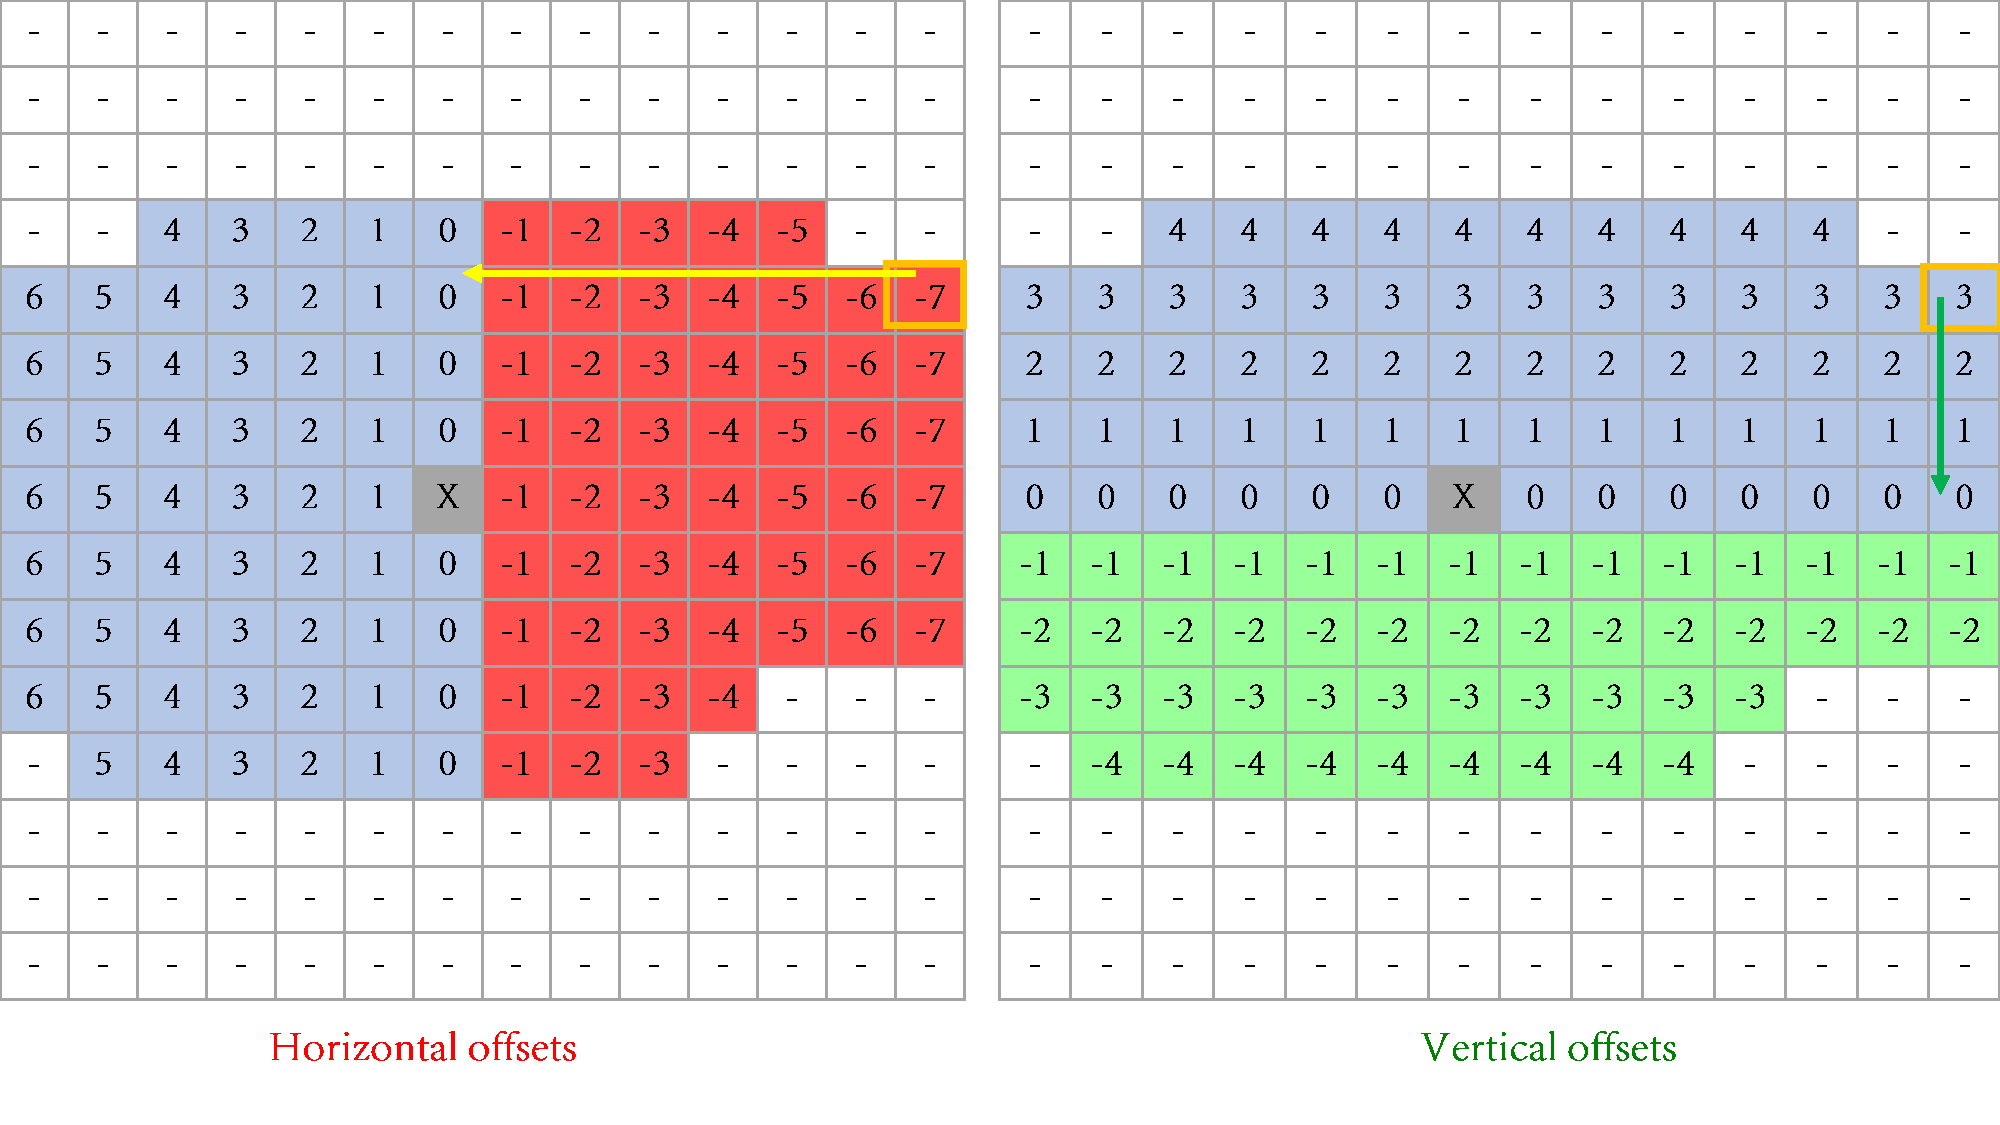
\includegraphics[width = \textwidth]{Graphics/Data_Representation/c2e_vis_flipped}
        \label{fig:c2e_vis_flip}}
        \caption[Center to End Encoding with Direction Recovering] {Illustration of center-to-end encoding and direction recovering a) shows a center-to-end encoding b) shows the offset directions recovered by inverting the offset values in center-to-end encoding}
        \label{fig:c2e_vis_pixels}
\end{figure}



\subsubsection{Euclidean Encoding}

Another way of encoding offset vectors is encoding euclidean distance. Given a pixel position, euclidean distance to corresponding instance center point is calculated and encoded at the same pixel location.  In such a representation, the direction is not considered at all as encoded value is calculated as a euclidean distance between given pixel position $(i,j)$ and corresponding center point $C_{k}(x_{1}, y_{1})$. This information can then be directly encoded in a single channel. Although a simple representation, it may not be the most effective and would also require an additional computational overhead by explicitly projecting each pixel to the direction of each center point in an image for calculating the distance between pixel position and center. Therefore, resulting in a single channel offset representation for generating groundtruth labels but is more ambiguous and demands extra computational expense. Visualisation of such representation can be seen in the figure \ref{fig:euc_img_vis}.

\begin{figure}[!ht]
%\centering
        \subfigure[End-to-End Encoding]{
        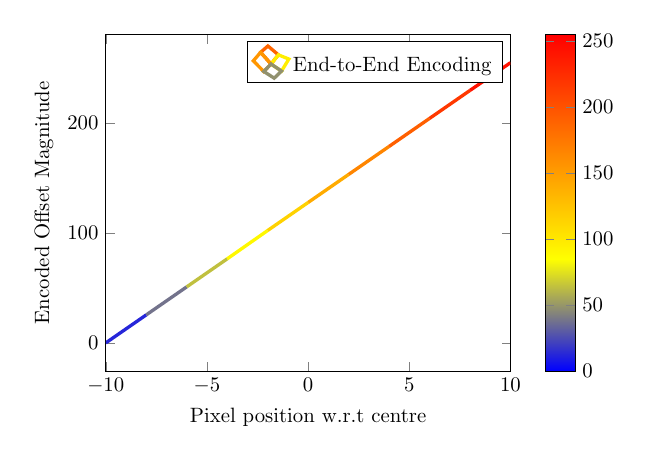
\begin{tikzpicture}[every axis/.style={
                xmax=10,%
                xmin=-10,%
                ylabel={Encoded Offset Magnitude },%
                xlabel={Pixel position w.r.t centre },%
                ytick={}
                }, scale=0.75]
                	\begin{axis}[colorbar]
                		\addplot[mesh, ultra thick,  width= \textwidth /2 ]         
                		plot coordinates { 
                            (-10, 0)
                            (-8, 25.5)
                            (-6, 51)
                            (-4, 76.5)
                            (-2, 102.3)
                            (0, 127.8)
                            (2, 153.3)
                            (4, 178.8)
                            (6, 204.3)
                            (8, 229.8)
                            (10, 255)
                        };;
                        \addlegendentry{ End-to-End Encoding}
                	\end{axis}
                \end{tikzpicture}
        \label{fig:e2e_plt_vis}}
        \subfigure[Center-to-End Encoding]{
        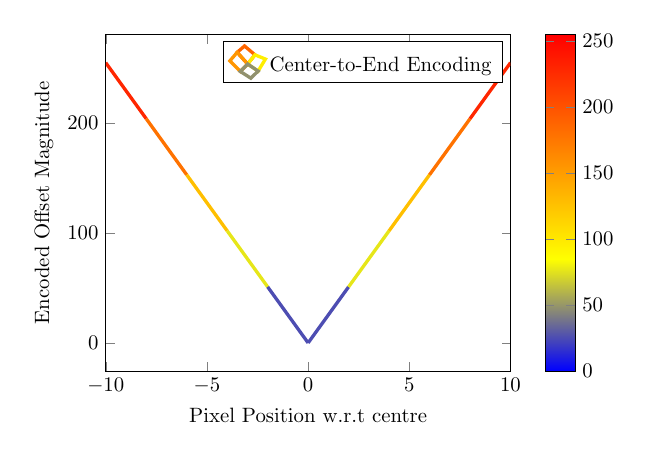
\begin{tikzpicture}[every axis/.style={
                xmax=10,%
                xmin=-10,%
                ylabel={Encoded Offset Magnitude},%
                xlabel={Pixel Position w.r.t centre },%
                ytick={}
                }, scale=0.75]
                	\begin{axis}[colorbar]
                
                		\addplot[mesh, ultra thick]         
                		plot coordinates {
                            (-10,255)
                            (-8,204)
                            (-6,153)
                            (-4,102)
                            (-2,51)
                            (0,0)
                            (2,51)
                            (4,102)
                            (6,153)
                            (8,204)
                            (10,255)
                        };;
                          \addlegendentry{Center-to-End Encoding}
                	\end{axis}
                \end{tikzpicture}
        \label{fig:c2e_plt_vis}}
            \caption[Plots representing Encoded Values]{Plots representing encoded value patterns a) shows end-to-end encoding where offset values increases linearly between either ends b) shows plot for center-to-end encoding where value increases monotonically in either directions around center point.}
    \label{fig:encodings_plots}
\end{figure}


















% !TeX root = ../thesis.tex

\chapter{Experimental Setup}
\label{sec:experimentatl_setup}


This chapter aims to define network architecture implementation details as well as experimental setup for panoptic segmentation architecture. Furthermore, it defines specifications for hyper-parameters. Hyper-parameter manipulation among
the experiments is kept to a minimum to ensure comparability and meaningful evaluation of the results.


\section{Network Architecture}


Typical approaches for instance and semantic segmentation have diverged in literature and each task usually
adopts fundamentally different kind of network architecture. There has not been many approaches that deal with both segmentation modalities following a similar approach. However, panoptic segmentation has been introduced as a unified segmentation task \cite{DBLP_panootic_seg:journals/corr/abs-1801-00868} which demands to tackle panoptic segmentation task within a single network architecture. To this end a unified network architecture has been implemented. 


Panoptic segmentation architecture implemented during the course of this master thesis relies on feature extractor based on a modern semantic segmentation architecture called \textit{DeepLab} \cite{Deeplabv3+:journals/corr/abs-1802-02611}. This semantic segmentation architecture has an encoder-decoder structure as shown in figure \ref{fig: deeplab_diag} that helps in gradually recovering spatial resolution and results in better recovered boundaries between different semantic classes. Deeplab also uses a combination of \textit{depth-wise separable convolutions } and \textit{atrous convolutions} as shown in \ref{fig:Depthwise_sep_conv} and \ref{fig:atrousconv} respectively. A depth-wise separable convolution that uses atrous convolutions i.e. convolution filters with padded zeros between learnable kernel values is called \textit{atrous separable convolutions} which has been explained in section \ref{subsec:atroussepconv}. Additionally, it employs a special kind of pooling module that applies multiple parallel atrous convolutions at different rates and concatenates them to collect the features from an input feature map, which is equivalent to pooling features at multiple spatial resolutions, hence equivalent to a \textit{feature pyramid}. This pooling module has been called \textit{Atrous Spatial Pyramid Pooling Module} (ASPP) and is augmented at the latent space of encoder. Owing to the above mentioned modules, deeplab is considered to be one of the sophisticated semantic segmentation architecture that utilizes efficient convolution operations, with dense feature extracting modules and encoder-decoder structure that aids semantic segmentation like tasks. A typical deeplab architecture has been shown in the figure \ref{fig: deeplab_diag}. 



\begin{figure}[!ht]
%\centering
\subfigure[Depth-wise Separable Convolution]{
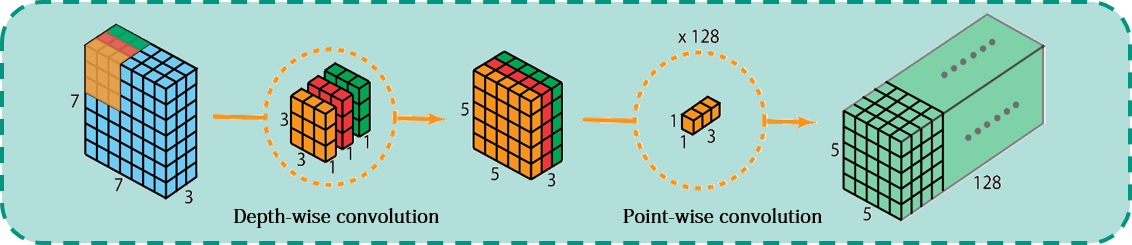
\includegraphics[width = \textwidth ]{Graphics/Experimental_Setup/Depthwise Seperable Convolution}
\label{fig:Depthwise_sep_conv}}

\subfigure[Atrous Convolutions]{
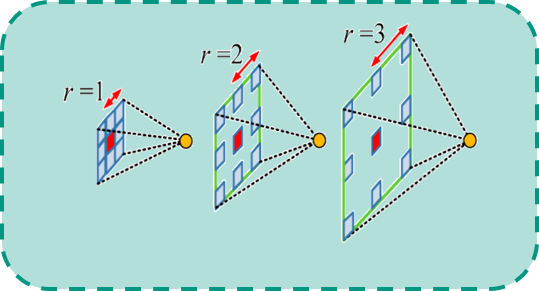
\includegraphics[width = \textwidth / 2 ]{Graphics/Experimental_Setup/atrous_conv}
\label{fig:atrousconv}}
\subfigure[Atrous Spatial Pyramid Pooling]{
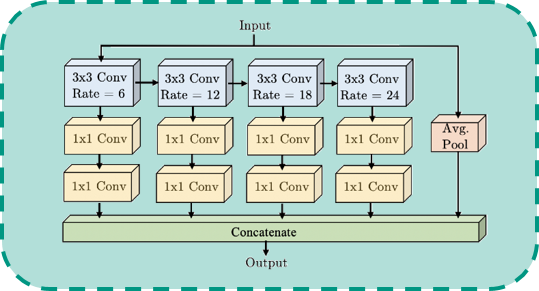
\includegraphics[width = \textwidth / 2 ]{Graphics/Experimental_Setup/atrous_spatial_pyramid_pooling}
\label{fig:aspp}}
\caption[Features of Deeplab ] {Illustration of some interesting features from DeepLab a) shows an illustration of a depth-wise separable convolution - a combination of depth-wise convolution followed by a point-wise convolution \cite{DEPSEPCONV} b) shows atrous convolutions - where zeros are padded in between learnable kernel filters, where rate is represented by \textit{r} and multiple filters with variable rates have been shown \cite{ATROUSCONV} c) represents a \textit{atrous spatial pooling module} - where pooling is implemented as parallel atrous convolutions at different rates - equivalent to pooling features from input feature maps at different resolutions \cite{Artacho2019WaterfallAS}}
\label{fig:features_deeplab}
\end{figure}

Due to aforementioned characteristics, panoptic architecture has been implemented on top of feature extractor from deeplab. Presented network architecture is hugely inspired by a very recently proposed \textit{Panoptic-deeplab}, a bottom-up architecture which attempted to solve panoptic segmentation task by predicting center points for instances and offset vectors.

\begin{figure}[!ht]
\centering 
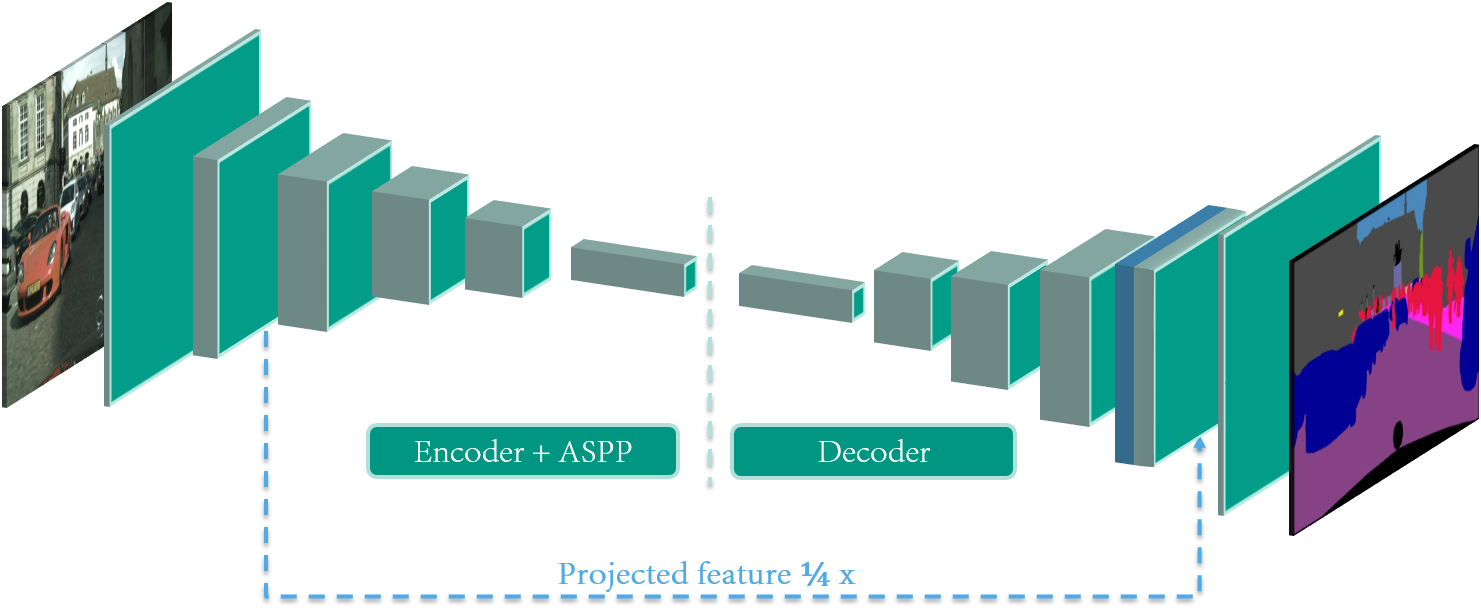
\includegraphics[width = \textwidth]{Graphics/Experimental_Setup/deeplab_image} 
\caption[DeepLab Architecture]{Illustration of DeepLab architecture showing encoder- decoder structure and projected features and atrous spatial pyramid pooling Module (ASPP)}
\label{fig: deeplab_diag} 
\end{figure}

The implemented architecture has been built on top of a deeplab architecture which aims to solve semantic segmentation in an encoder-decoder configuration, where decoder gradually recovers the spatial resolutions by generating output logits equivalent to input image resolution as shown in figure \ref{fig: deeplab_diag}. The panoptic segmentation network extends the deeplab network by an additional decoder branch in addition to the semantic segmentation branch. This newly extended branch is further extended by two heads, where one is responsible for center point predictions and other for offset vector predictions. Each decoder augments its own atrous spatial feature pyramid module that exploit their inherent feature pyramid effect to pool features from latent space independently. Additionally, features from lower layers in encoder are projected to higher layers in both decoders at same spatial resolution i.e. at $1/4$ and $1/8$ of input resolution. These projected features act as skip connections, that feed low-level information from lower layers to higher layers for reconstructing better spatial information. Additionally, during back-propagation parameters from lower layers can exhibit their direct dependency to output logits and can be tuned accordingly. For more details about the implemented architecture, reader is refereed to \cite{Cheng_2020_CVPR}. Another highlight of using such deeplab based semantic segmentation feature extractor is that it exploits a variant of \textit{Xception network} \cite{DBLP:journals/corr/Chollet16a} that is well-suited for learning semantic and pixel-level representations. Adaptations in the xception network and further details about the utilized network architecture have been presented in the figure \ref{fig: modifiedxception}. Further details on how class-agnostic instance segmentation has been achieved is provided in the following chapter.


\begin{figure}[!ht]
\centering 
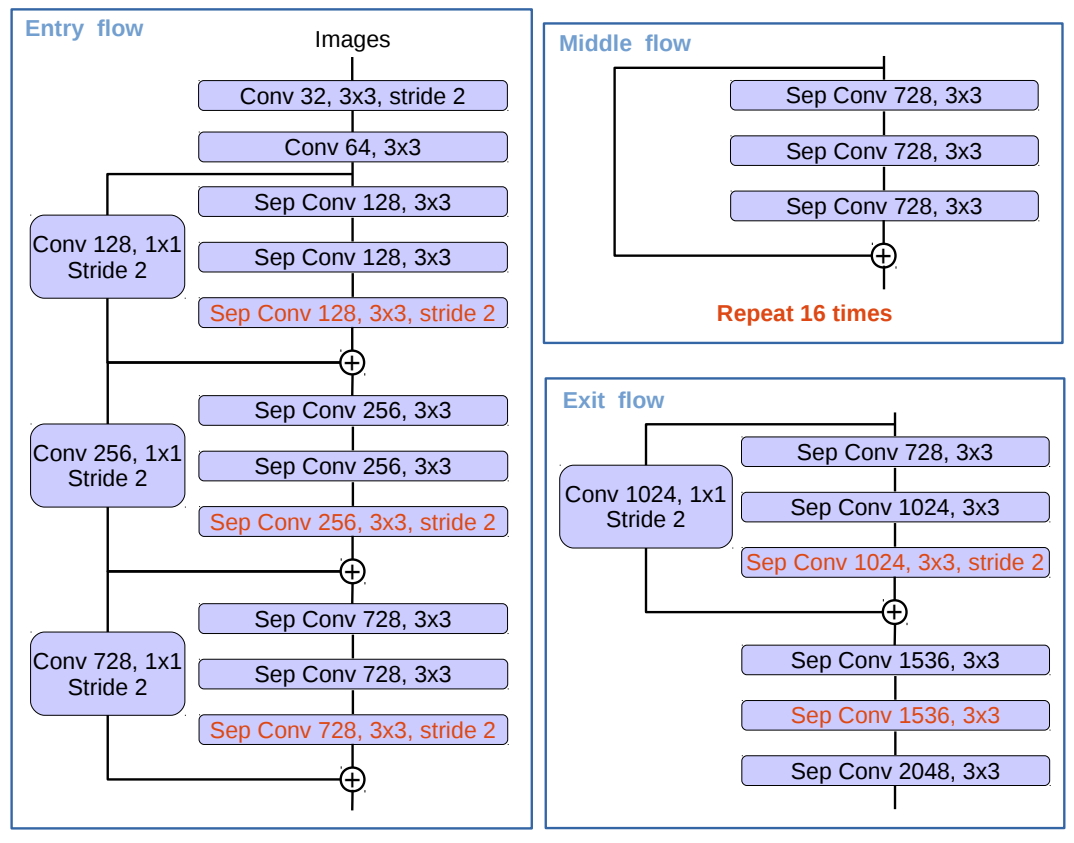
\includegraphics[width = \textwidth]{Graphics/Experimental_Setup/xception} 
\caption[Variant of Xception Architecture]{Figure shows a variant of xception network architecture that is employed in DeepLab feature extractor - showing  (1) more layers in comparison to originally proposed network \cite{DBLP:journals/corr/Chollet16a} (2) max pooling operations are replaced by depth-wise separable convolutions with striding (3) extra batch normalization and ReLU added after each depth-wise convolution. \cite{Deeplabv3+:journals/corr/abs-1802-02611}}
\label{fig: modifiedxception} 
\end{figure}





\bigskip
\begin{sidewaysfigure}
\centering 

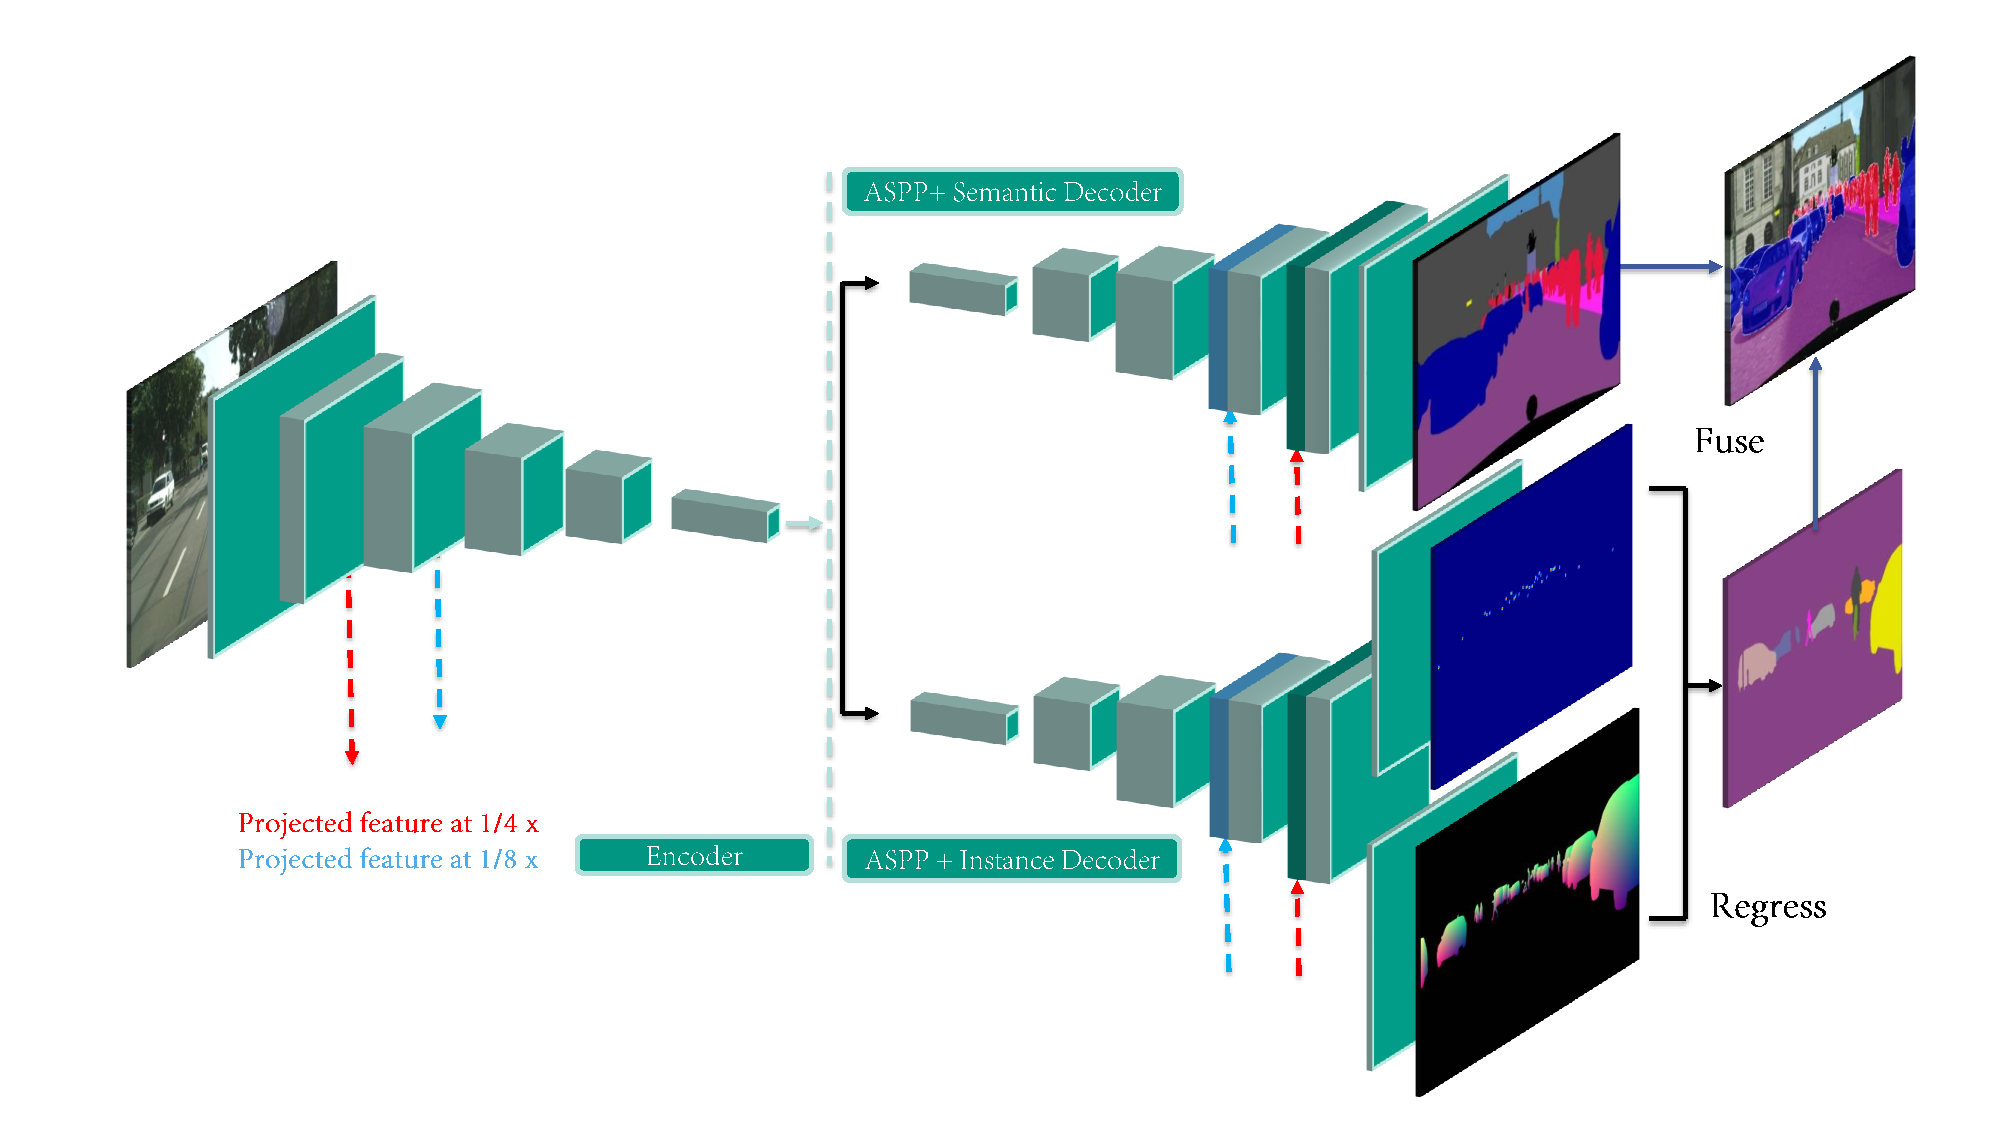
\includegraphics[width = \textwidth]{Graphics/Experimental_Setup/panoptic_deeplab.pdf} 
\caption[Panoptic DeepLab Architecture]{Illustration of Panoptic-DeepLab architecture- showing (1) encoder-decoder structure (2) dual decoder and dual ASPP modules each for semantic decoder and instance decoder (3) projected features at $1/4$ and $1/8$ spatial resolutions (3) instance decoder extended further by two task specific heads for center point predictions and offset vectors prediction.}
\label{fig: panopticdeeplab_diag} 
\end{sidewaysfigure}

\subsection{Semantic Segmentation Head}
Semantic segmentation head as seen in figure \ref{fig: panopticdeeplab_diag} employs \textit{weighted bootstrap cross entropy loss} during training as proposed by \cite{DBLPDeeperLab:journals/corr/abs-1902-05093}. The loss has shown to improve over vanilla bootstrapped cross entropy loss since, each pixel is weighted differently \cite{DBLP:journals/corr/WuSH16b}. Semantic segmentation head is dedicated to learn semantic segmentation of the scene for both \textit{things} and \textit{stuff} classes. 

\subsection{Center Prediction Head}

To learn the center points for instances, groundtruth labels are generated by calculating center of mass for each instance individually followed by an encoding with a standard $2D$ gaussian distribution around each calculated center of mass. To learn such a representation, during training \textit{ Mean Squared Error} (MSE) criterion has been employed to minimize the distance between the predicted heat-map and a groundtruth heat-map \cite{DBLP:journals/corr/TompsonJLB14}. 

\subsection{Offset Prediction Head}

Offset vectors ground-truth labels are generated by calculating distance of each \textit{things} class pixel to its center. By doing so, each pixel encodes distance to it corresponding center in vertical and horizontal direction independently in one channel. $L1$- loss has been employed for training such offset vector representations. During inference, predicted offsets and center points are grouped together to generate class-agnostic instance masks using a simple regression operation.


\section{Evaluation Metrics}


\gls{pq} was the first panoptic segmentation evaluation metric introduced along-with reviving the unified segmentation task \cite{DBLP_panootic_seg:journals/corr/abs-1801-00868}. During evaluation, for each segment a matching is employed that splits the predicted segments in: \gls{tp}, \gls{fp}, \gls{fn} corresponding to matched pairs, unmatched predicted segments and unmatched groundtruth segments. Given the above matching criteria \gls{pq} can be defined as follows:

\begin{equation}\mathrm{PQ}=\frac{\sum_{(p, g) \in T P} \mathrm{IoU}(p, g)}{|T P|+\frac{1}{2}|F P|+\frac{1}{2}|F N|}\end{equation}

\gls{pq} can be seen as a multiplication of two factors:

\begin{equation}\mathrm{PQ}=\frac{\sum_{(p, g) \in T P} \operatorname{IoU}(p, g)}{|T P|} \times \frac{|T P|}{|T P|+\frac{1}{2}|F P|+\frac{1}{2}|F N|}\end{equation}

where the first term has been called \gls{sq} which corresponds to average \gls{iou} of matched segments and second term corresponds to \gls{rq} which is the widely employed F1-score.
However, \gls{pq} treats all segments equally regardless of area i.e.  $10\times10$ and $2000 \times 2000$ pixels are weighted equally \cite{DBLP_panootic_seg:journals/corr/abs-1801-00868}, \cite{DBLPDeeperLab:journals/corr/abs-1902-05093}. 

Therefore, \gls{pc} was recently proposed as an evaluation metric for panoptic segmentation task that remedies the aforementioned problem on equal weighting irrespective of segment size. \gls{pc} can be defined as follows: 

\begin{equation}C o v_{i}=\frac{1}{N_{i}} \sum_{R \in S_{i}}|R| \cdot \max_{R^{\prime} \in S{i}^{\prime}} I O U\left(R, R^{\prime}\right)\end{equation}

\begin{equation}N_{i}=\sum_{R \in S_{i}}|R|\end{equation}

\begin{equation}P C=\frac{1}{C} \sum_{i=1}^{C} C o v_{i}\end{equation}

where $S_{i}$ and $S_{i}^{\prime}$ are groundtruth and predicted segments of given class $i$, and $N_{i}$ is the number of pixels in groundtruth region. \gls{pc} can be calculated by computing the average of $Cov_{i}$ over $C$ number of semantic classes. Reader is refereed to \cite{DBLPDeeperLab:journals/corr/abs-1902-05093} for further information on evaluation metric. 

For evaluation purposes, \gls{pc} has been chosen to report and document evaluation and comparison of experiments for presented work.

\section{Hyper-parameter Specifications}

This section specifies hyper-parameters used in experiments carried out during the scope of this work. Since, a suitable hyper-parameter configuration is critical for efficient training, most of the below mentioned hyper-parameters were chosen based on best practices in the literature and were defined at an early stage of this work.  Hyper-parameter manipulation among the experiments is kept to a minimum to ensure comparability and meaningful evaluation of the results. However some parameters used in post-processing and did not have an effect on training process were chosen after extensive evaluation to squeeze best performance.

Additionally, due to limited computational resources, two stage training process has been adapted, where first stage has relatively larger batch size with smaller image crops to enable focus on smaller details and make use multiple samples in each step. To learn a holistic scene representation, a larger crop size is adapted while sacrificing on batch size in the subsequent stage. 


\paragraph{Learning Rate}

For a learning process, learning rate defines how fast the network weights are adapted with respect to gradient in a single optimisation step. See section \ref{subsec:learningnopt} for more details. A higher learning rate results in faster adaptation of weights, however it might result in a sub-optimal solution. Usually, a very small learning rate is adapted to slowly converge towards an optimal solution whilst avoiding local-minimum. Learning rate for all the experiments carried out during presented work is chosen to be $0.001$.

\paragraph{Batch Size}

Batch size defines the number of samples chosen for each step during a learning process. The network parameters are optimised during each iteration with respect to number of samples at hand, defined by batch size parameter. Usually, a relatively higher batch size is preferred to include diversity and make use of GPU parallelism to speed up learning process. In the first stage a batch size of $4$ is chosen, while in the second stage batch size is chosen to be $1$.

\paragraph{Input Shape}

All the input images that are passed through the network are expected to be of same input resolution. Deeplab architecture adapts to various input resolutions. In the first stage of training process, input images are cropped to $769\times769$ resolution, whereas, in the second stage input images are cropped to $1025\times1025$ spatial resolution.

\paragraph{Number of iterations}

Number of update steps in a training process are defined by number of iterations. In the presented work, training is carried out in two stages. For the first stage, number of iterations are set to be $150,000$ while in the second stage (with larger crop size and single batch size) number of iterations are set to be $50,000$.

\paragraph{Optimizer}

To ensure compatibility and standardized comparison, all the reported experiments carried out during the course of presented work employed \textit{Adam} as an optimizer \cite{Goodfellow-et-al-2016} with \textit{poly learning rate decay}. See section \ref{subsec:learningnopt} for more details.  


\paragraph{Regularization}

To avoid over-fitting and improve generalization presented work uses batch normalization, dropout and weight decay for regularization purposes. 

\paragraph{Number of project features}

As mentioned in the previous section of this chapter, the network makes use of low-level features by sharing information between encoder and decoder modules i.e. low-level features from encoder (at spatial resolution $1/4$ and $1/8$ of original input size) are projected at the same spatial resolution in both decoders independently, as shown in the figure \ref{fig: panopticdeeplab_diag}. Before concatenating with decoder features the projected features are passed through a convolution operation to reduce number of channels (by a point-wise convolution) see section \ref{subsec:atroussepconv}, which defines the number of projected features. Number of projected features for semantic decoder are fixed to $32$ and $64$ at spatial resolution $1/4$ and $1/8$ of input size respectively. While, number of projected features for instance decoder are set $16$ and $32$ at spatial resolution $1/4$ and $1/8$ of input size respectively.


\paragraph{Center Pooling Kernel Size}

The network predicts a probability distribution around each center point, however it is desired to extract exact locations for each center prediction. To this end, max pooling is employed that only keeps the pixel location with maximum prediction confidence each kernel window. The size of this pooling kernel can be adapted. Since this is a post-processing step and does not influence learning, various kernel window sizes have been compared against each other and kernel window of $72\times72$ was observed to yield best results and was fixed for further experimental evaluations.

\paragraph{Number of Instances}

Another parameter that is part of post-processing step and does not affect learning process is the number of instances. After pooling the center points using a fixed kernel window, the number of filtered center points are limited by selecting top 200 centers according to their prediction confidence. 

\paragraph{Deep Learning Framework}

To implement bottom-up panoptic segmentation network architecture and to carry out experiments \textit{Tensorflow framework} has been used since it is highly flexible regarding implementation and provides extensive documentation. In addition, it provides an integrated tool called \textit{Tensorboard} that enables online monitoring and comparison between experiments. Therefore, network architecture implementation and conduction of experiments was carried out using Tensorflow framework.  






% !TeX root = ../thesis.tex

\chapter{Methodology}
\label{sec:methodology}

This chapter aims to describe the methodology adapted for generating panoptic segmentation. First section provides details about a structured approached employed to generate class-agnostic instance masks from predicted center points and offset vectors. Subsequently, it describes highly efficient merging operation between semantic and instance semantic segmentation to generate a unified and coherent panoptic scene representation.

\bigskip

\section{Approach}

 To generate a coherent and comprehensive representation of the environment under observation, it is desired to have a representation that not only describes semantic layout of the environment but also provides instance-level information on traffic participants. Further, it is desired to have a single representation that encodes both modalities and provides for a simple pixel-level expression of class label and instance id. By doing so, pixel-level fine-grained segregation of the scene can be achieved. To this end, a structured approach has been adapted to combine network predictions to achieve such a unified representation i.e. panoptic scene segmentation. General approach adopted for this purpose can be seen in the figure  \ref{fig:panoptic_seg_approach}. In figure \ref{fig: panopticdeeplab_diag}, it can be seen that the implemented network architecture adopts dual-decoder structure one for learning instance segmentation while the other learns pixel relationships. Furthermore, instance decoder is extended by two task specific heads for center point predictions and offset vectors predictions. In the first step, task specific outputs in instance decoder (center predictions and offset predictions) are combined to generate class-agnostic instance masks which makes use of a simple regression operation. Subsequently, the generated instance segmentation and semantic segmentation prediction from both decoders are combined. In the first step however, both predicted representations from instance decoder are pre-processed before the merging operation could begin. This has been explained in more detail in following sections independently for each prediction.

\begin{figure}[!ht]
    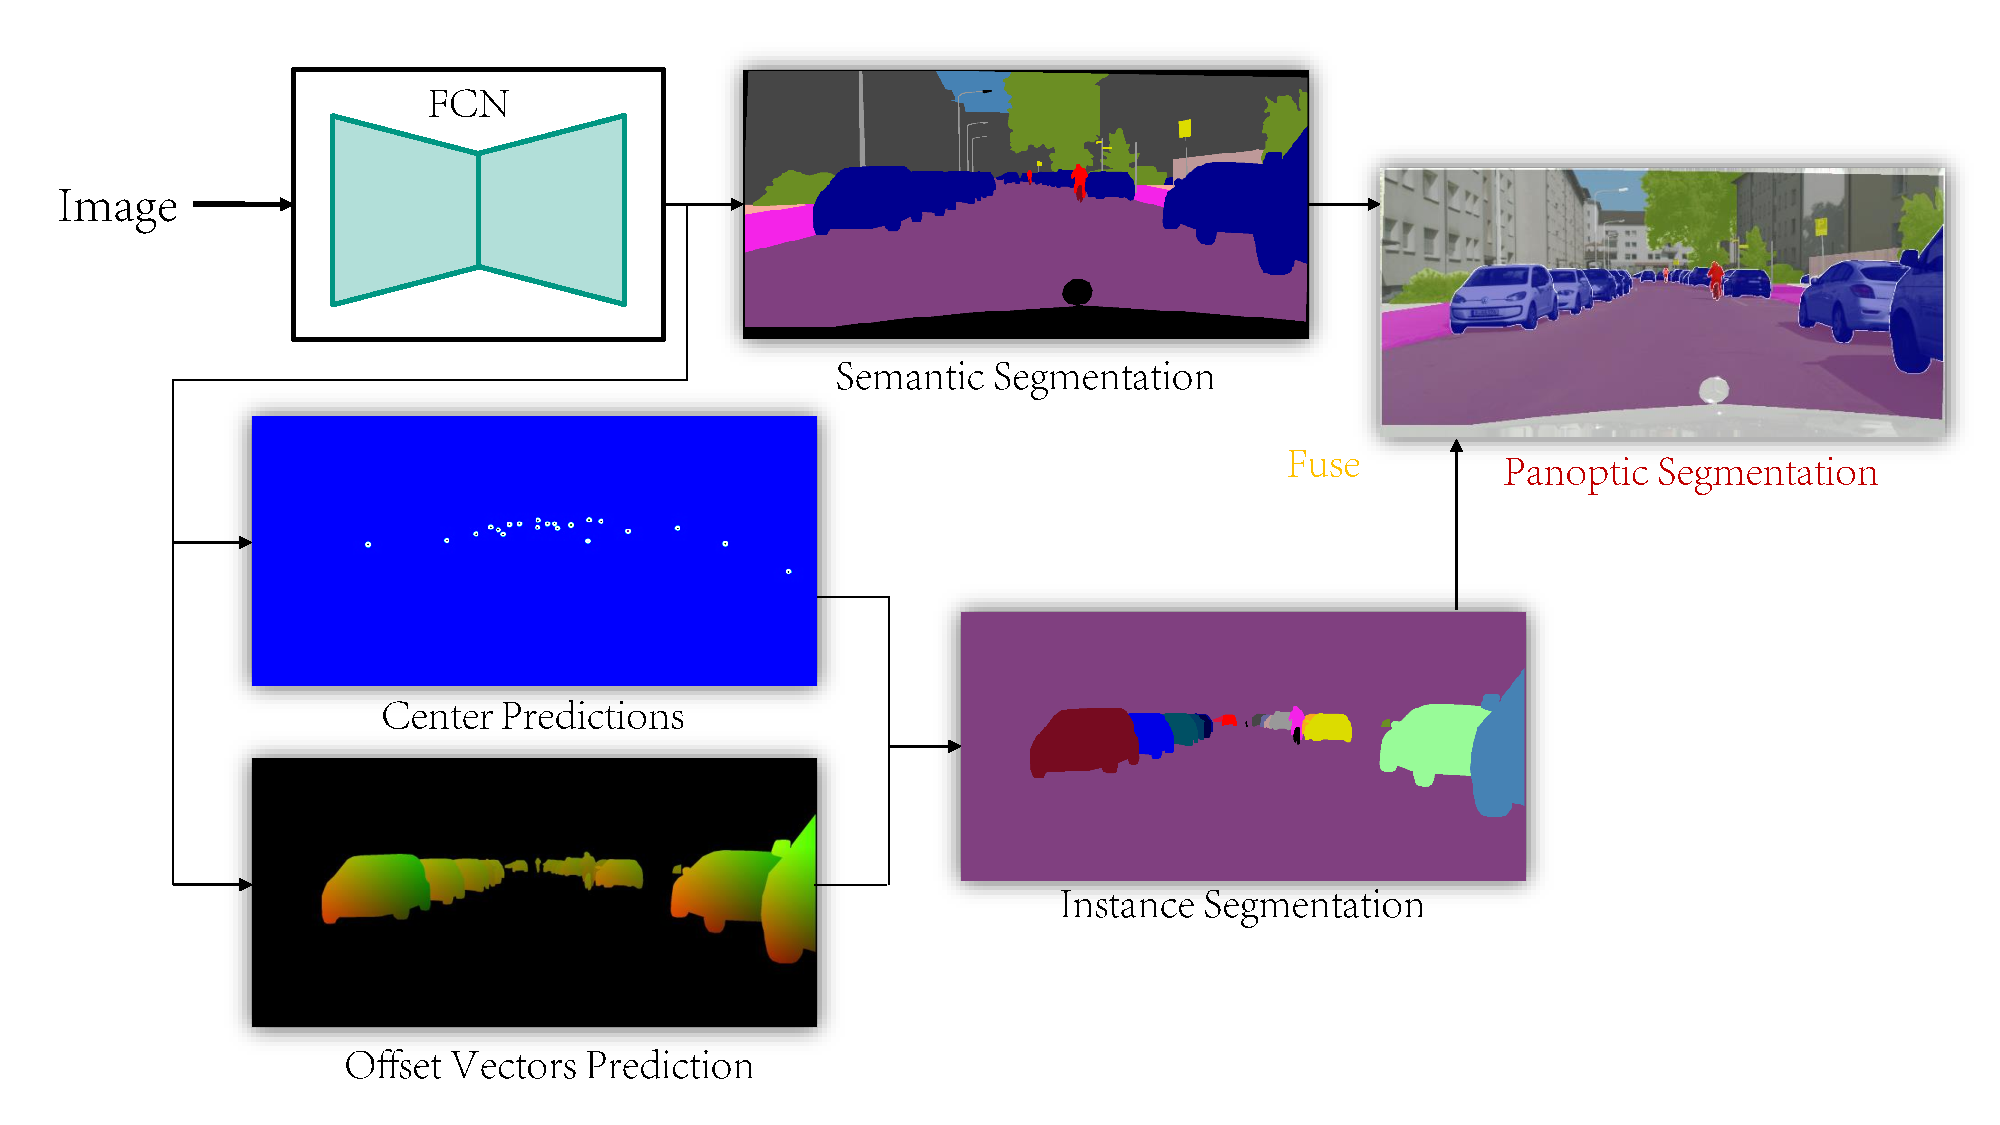
\includegraphics[width = \textwidth]{Graphics/Methodology/panoptic_seg_approach.pdf}
    \caption[Panoptic Segmentation Approach]{Illustration of general approach for panoptic segmentation - showing \gls{fcn} predicting 3 outputs where center points are offset representations combine to generate instance segmentation which in turn combines with semantic segmentation to generate panoptic segmentation.}
    \label{fig:panoptic_seg_approach}
\end{figure}


\subsection{Center Rendering}
\label{subsec:center_rendering}

During inference, center point predictions are pre-processed primarily for extracting exact center point locations out of center prediction (which is a probability distribution around center points). Furthermore, it is also desired to do a non-maxima suppression to avoid any false positives that might appear. Since, task specific head for center-point predictions is trained against a representation containing probability distributions around center-points of each \textit{things} class instance, therefore the output predicted by trained network also predicts a similar representation of probability distributions around probable center-points. Therefore, before a hough voting based grouping operation similar to \cite{Ballard1981} could be employed to generate class-agnostic instance segmentation, it is desired to extract exact pixel locations for each center point. 
To render exact center location and suppressing any false positives, following steps are performed:

\begin{enumerate}
    \item Threshold based non-maxima suppression.
    \item Max-pooling based non-maxima suppression.
    \item Filtering top-k number of pooled centers.
\end{enumerate}


\begin{figure}[!ht]
%\centering
    \subfigure[Predicted heatmap]{
        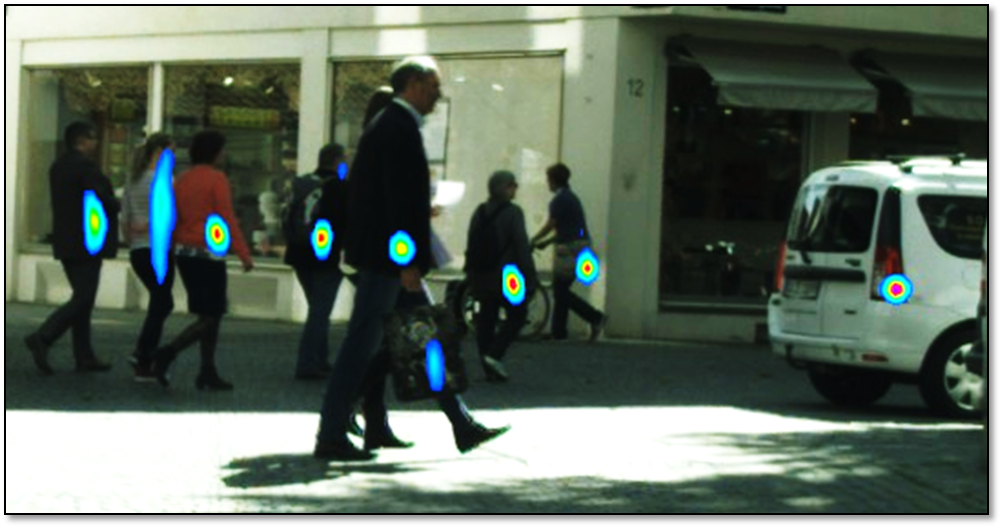
\includegraphics[width = \textwidth / 2 ]{Graphics/Methodology/Picture1}
        \label{fig:centerrawpred}}
    %\hspace{1pt}
     %add desired spacing between images, e. g. ~, \quad, \qquad, \hfill etc.
     %(or a blank line to force the subfigure onto a new line)
    \subfigure[Scaled and threshold at 0.39]{
        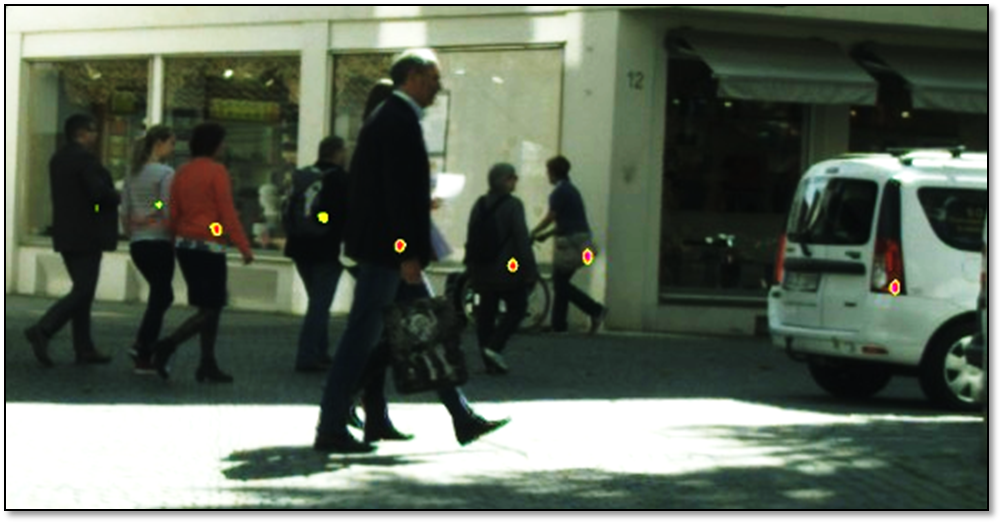
\includegraphics[width = \textwidth / 2 ]{Graphics/Methodology/Picture2}
        \label{fig:centerthreshold}}
    \subfigure[Max-pooling based NMS]{
        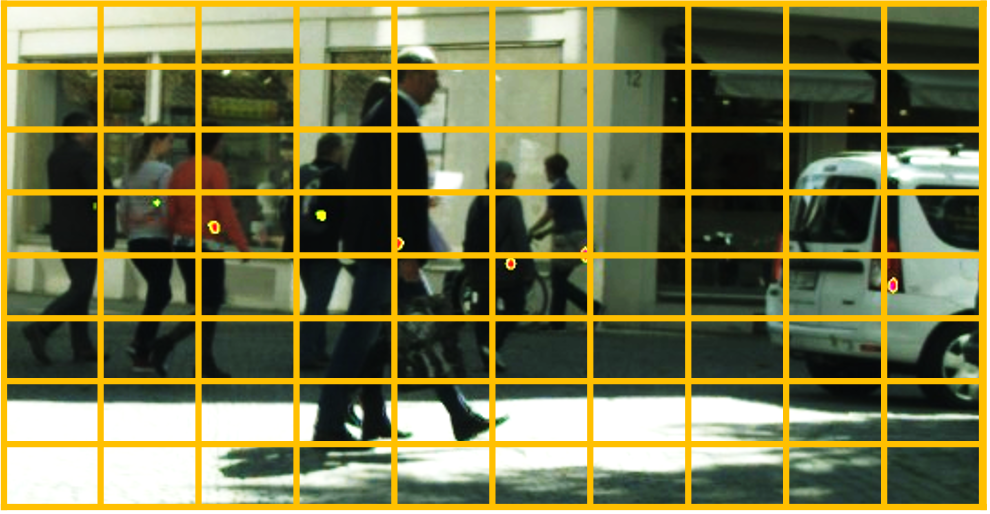
\includegraphics[width = \textwidth / 2 ]{Graphics/Methodology/Picture3}
        \label{fig:centermaxthreshold}}
%   \hspace{1pt}
    \subfigure[Extracted center locations]{
        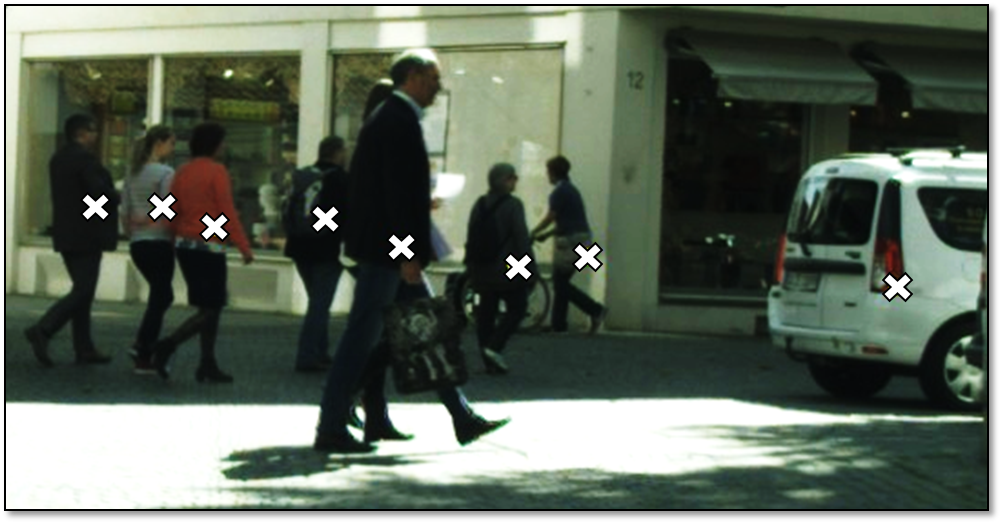
\includegraphics[width = \textwidth / 2 ]{Graphics/Methodology/Picture4}
        \label{fig:center_extracted}}
    \caption[Center Position Extraction ] {Raw center predictions from the network and subsequent steps for non-maxima supression and extracting exact center positions a) depicts raw predicted heatmap with centers represented by a probability distribution b) shows scaled and thresholded heatmap c) shows a non-maxima suppression (NMS) based on max-pooling with a fixed kernel window d) shows exact center locations extracted using max-pooling by keeping only highest prediction location in each kernel window.}
    \label{fig:centerpred_preprocessing}
\end{figure}

Center point prediction head in the network predicts a representation where each center point has been predicted as a probability distribution around probable center, visualisation of such output from network can be seen in figure \ref{fig:centerrawpred} where each distribution can be seen to extend over a number of pixels. It is desired to extract an exact number of center points with accurate locations. To this end, first the probabilities are scaled between $0-1$ and thresholded at $0.39$ , see figure \ref{fig:centerthreshold}. It was found that thresholding at $0.39$ resulted in acceptable trade-off between false positives and false negatives.   This is followed by a non-maxima suppression step which has been implemented efficiently as a max-pooling operation with stride of a single pooling window by keeping only the location of pixel with highest prediction confidence in each window as shown in figure \ref{fig:centermaxthreshold}, for further information see section \ref{subsec: pooling_operation}. This results in an effective non-maxima suppression resulting in unique center point locations which can be used for grouping offset representations to their corresponding centers. Additionally, maximum number of center-points are restricted to a highest of 200. Therefore, picking only the top-k center points from pooled centers where k in this case is chosen to be 50 or 200. The resulting center points after these operations are used for grouping offset vectors.




\subsection{Offset Directions}

In chapter \ref{sec:data_representation}, information about various data representations has been provided. In this work, various representations and encoding were conceptualized and implemented to generate datasets that were used to train the network. Section \ref{subsec:offsets}, describes few offset representation possibilities that are well-suited for representing pixel relationships to their center points. More specifically, it can be seen that end-to-end encoding can directly encode the distance and direction i.e. real offset with direction information required to reach its center point, see figure \ref{fig:e2e_vis_pixels}. On the other hand, center-to-end encoding only encodes the distance i.e  offset in terms of magnitude that is required to reach center without encoding direction, as visualised in figure \ref{fig:c2e_vis_pixels}. Similarly, euclidean encoding directly encodes the euclidean distance to the center point without being aware of the direction information, as shown in figure \ref{fig:euc_img_vis}. Nevertheless, efficient and precise grouping of pixels to corresponding centers demands direction information. End-to-end encoding inherently encodes direction and therefore does not require any additional processing to initiate grouping operation. However, center-to-end encoding does not include direction information and therefore demands an orientation correction for offset vectors. During inference, network predicts semantic segmentation, center predictions and offset predictions. Since network also predicts on whereabouts of center positions for each instances, it also gives the possibility to correct the orientation of offset vectors with respect to each center point. To this end following steps are performed:
\bigskip

\begin{enumerate}
    \item Extract exact center points using \gls{nms}. 
    \item In horizontal offsets, invert direction of pixel values on the right side of center point.
    \item In vertical offsets, invert direction of pixel values below the center point.
\end{enumerate}

\begin{figure}[!ht]
    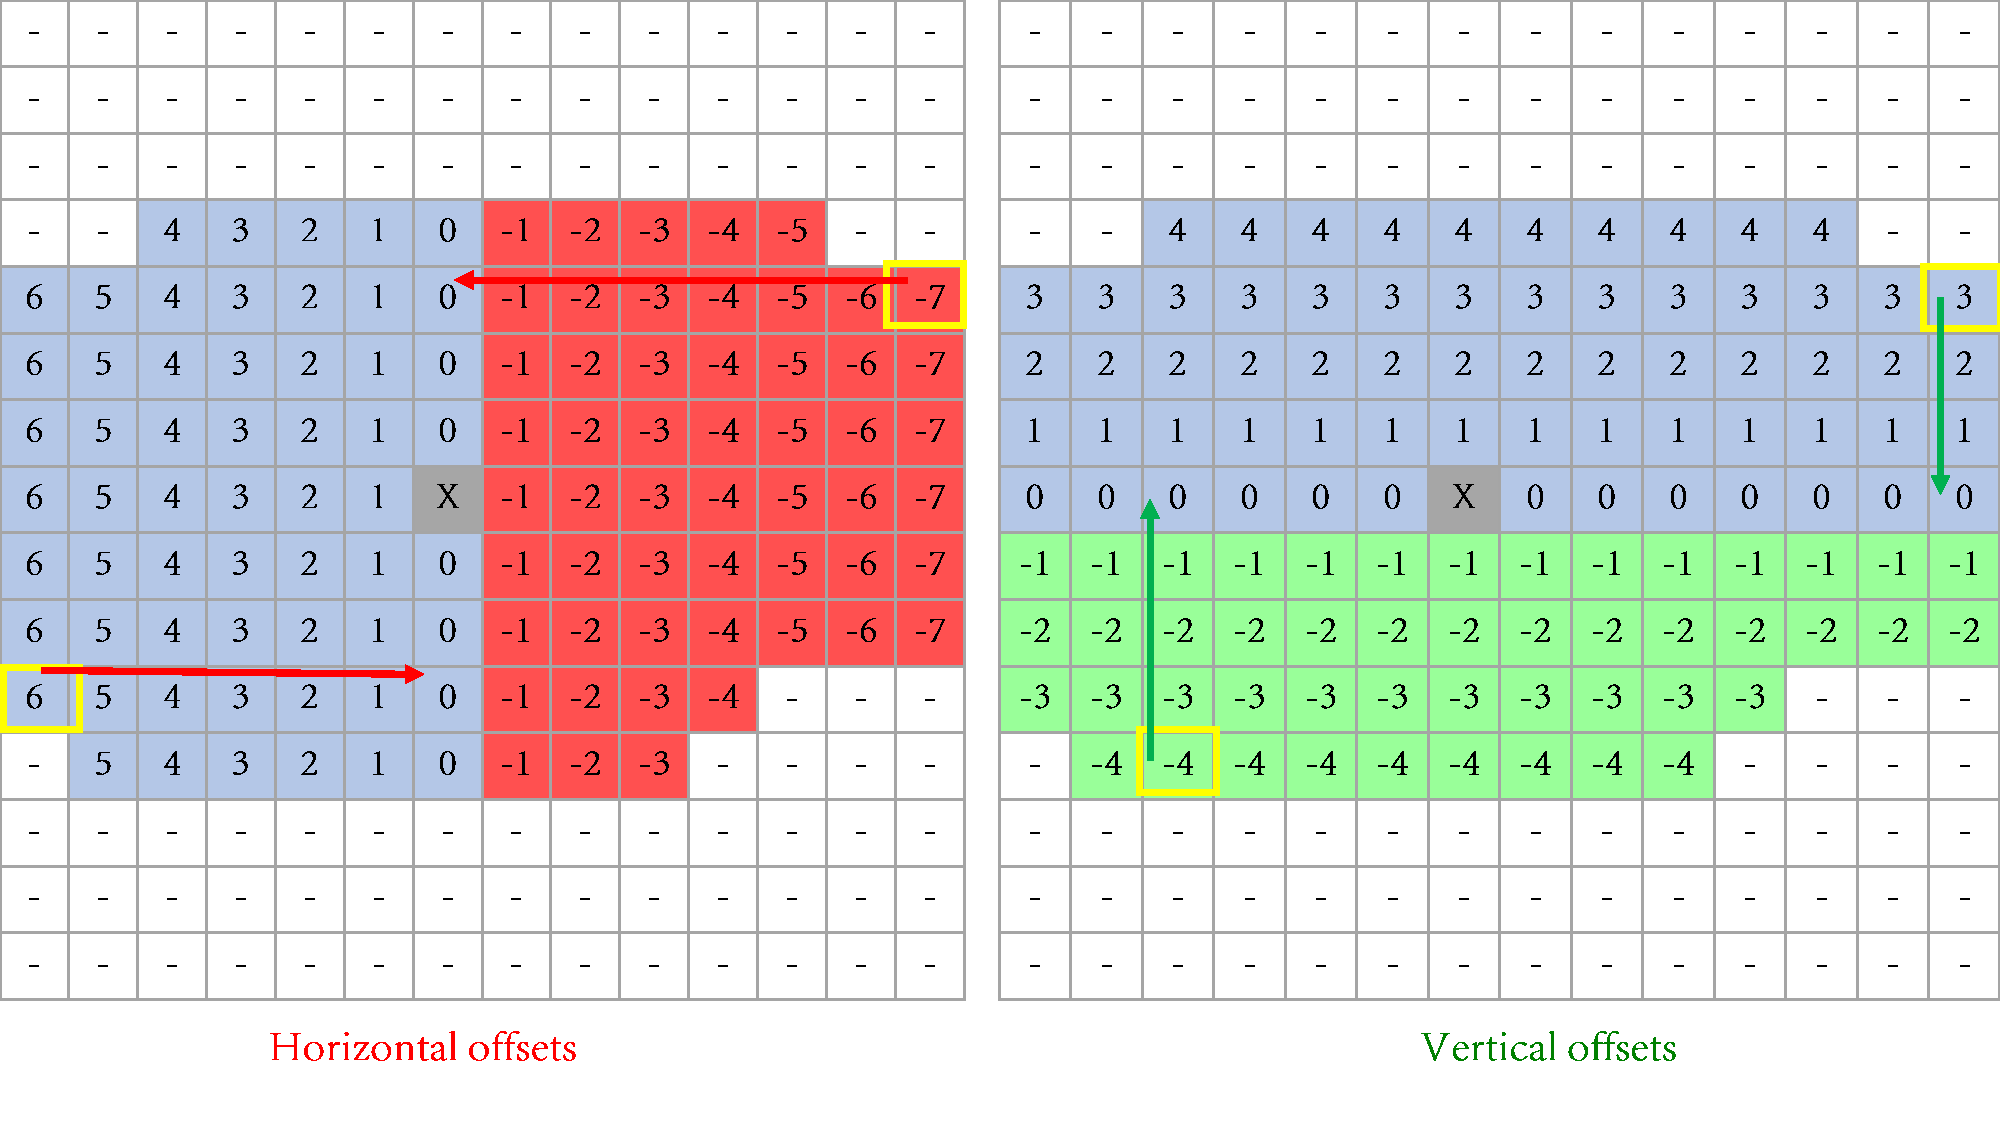
\includegraphics[width = \textwidth]{Graphics/Methodology/extra_offsets.pdf}
    \caption[Offset Vectors with Recovered Direction]{Illustration of offset vectors with recovered directions - recovered direction is based on the center point predictions, where offset vectors in horizontal and vertical offsets are flipped on one side of the predicted center (recovering the real direction of offset required to reach center)}
    \label{fig:offsets_pixels_recovered}
\end{figure}

\subsection{Instance Grouping}
\label{subsec:regression_approach}

First exact center points are achieved using non-maxima suppression as explained in section \ref{subsec:center_rendering}. Given a center point location, pixel values on the right side of center point in horizontal offsets are inverted which corresponds to a negative offset required to reach the center point if the encoding is center to end. Similarly, pixel values below this center point in vertical offsets are inverted to change direction which again indicates that a negative offset in vertical direction is required to reach center point. This is done independently for each center point. After this operation, each pixel in offset representation encodes the actual offset and direction required to reach center. Visualisation of which can be seen from the figure \ref{fig:offsets_pixels_recovered}, where each pixel in either of the offset predictions has corrected directions and essentially points toward center point.


Hence, to generate the instance segmentation output from processed predicted representation, first exact center pixel positions for all center points of potential instances are recovered. And offset vectors are ensured to point correctly in real offset direction i.e, if the encoding is end-to-end, see section \ref{subsec:e2e} - no processing required on the other hand, if encoding is center-to-end as described in section \ref{subsec:c2e} - offset vectors are inverted on one side in both horizontal and vertical offset predictions as illustrated  in figure \ref{fig:c2e_vis_pixels}. The resulting offset predictions then exhibit a predicted offset to their corresponding center pixel with true direction as visualised in figure \ref{fig:offsets_pixels_recovered}.  

\begin{figure}[!ht]
    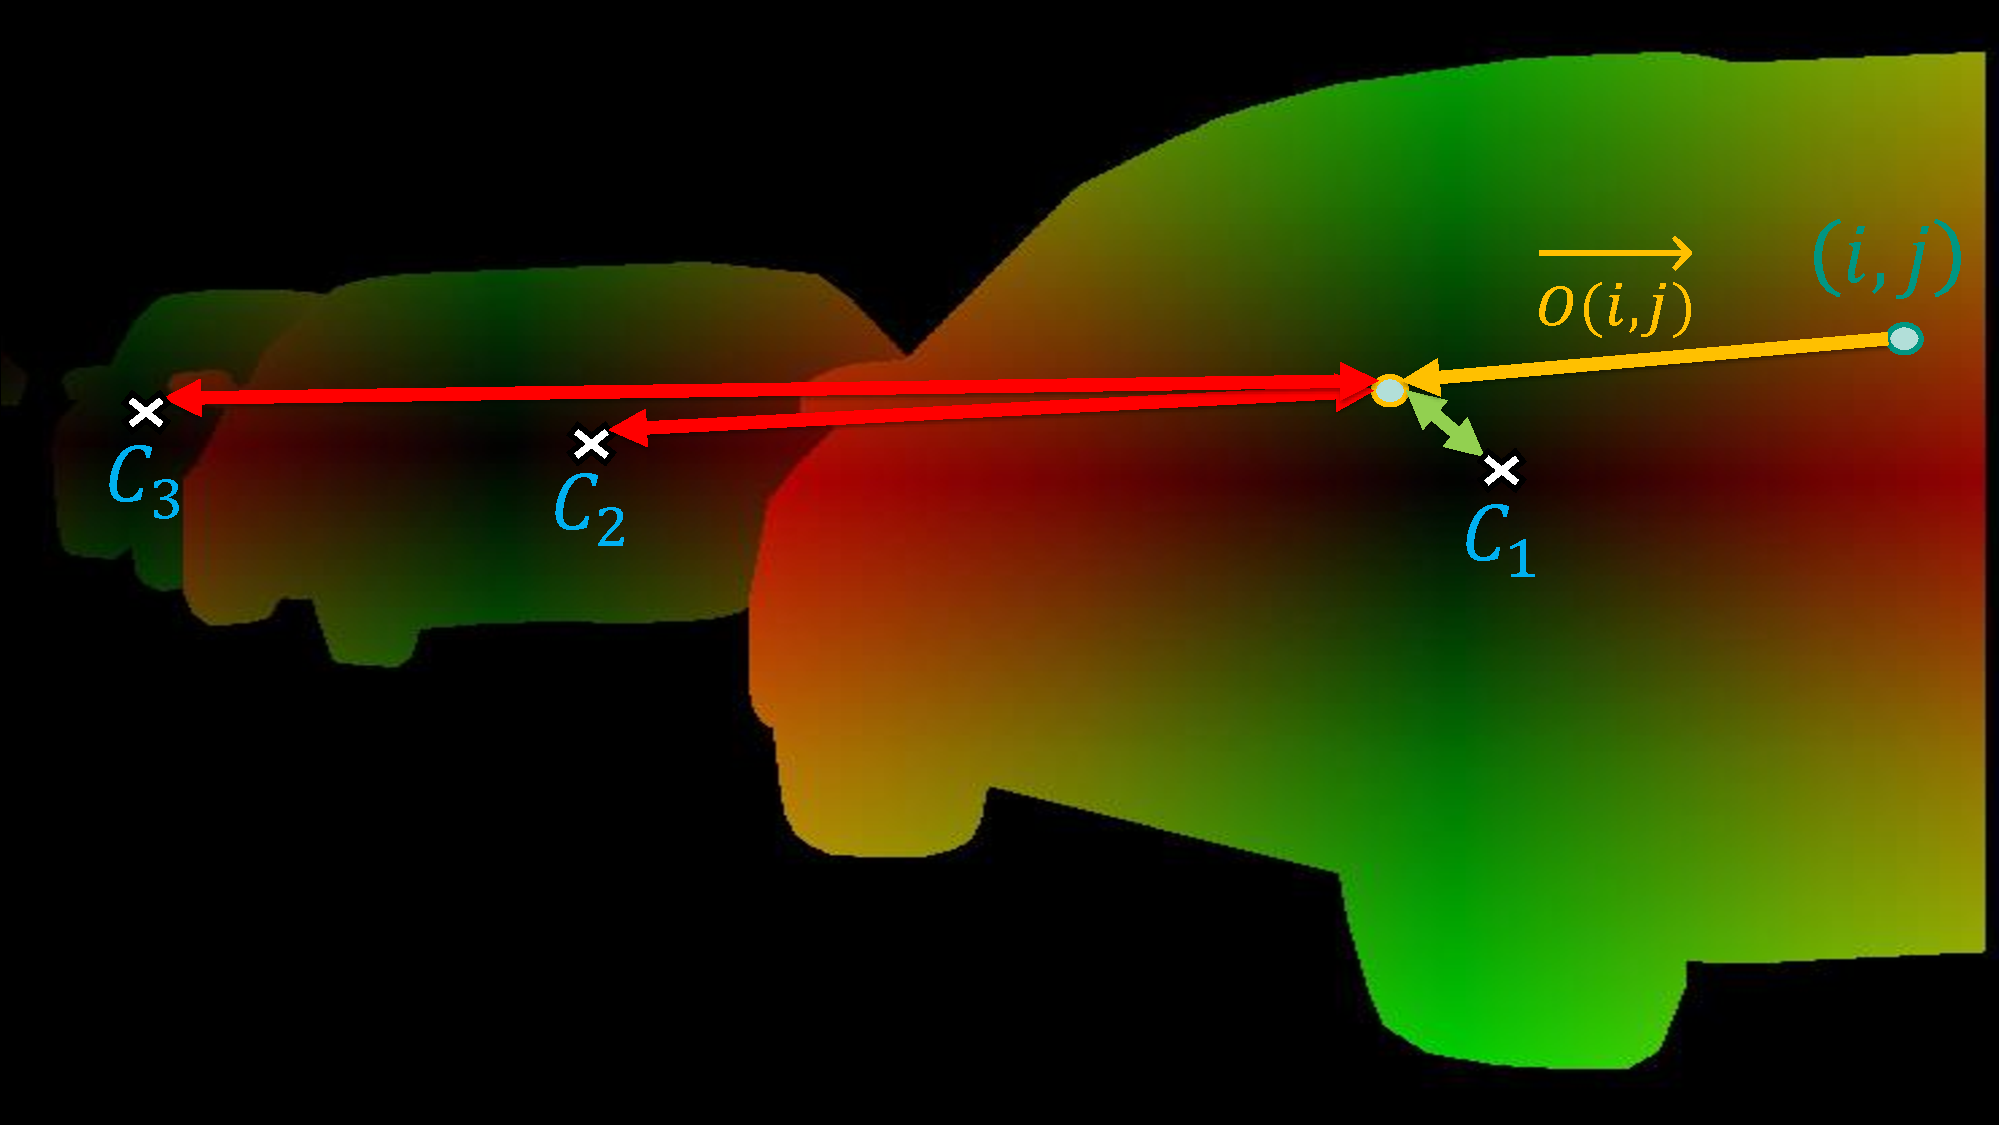
\includegraphics[width = \textwidth]{Graphics/Methodology/instance_regression.pdf}
    \caption[Regression Approach to Generate Instance Masks]{Illustration of regression operation employed to generate instance masks using center point positions and offset vector representations. Given a pixel at position $(i,j)$, it is moved by the predicted offset to a new location. This new location is compared to all the center positions, the pixel in the end is assigned to the center closest to the new location.}
    \label{fig:regression_approach}
\end{figure}

Given the processed representations as described, pixel grouping is then posed as a simple regression problem to generate class-agnostic instance masks as described by equation \ref{eq:regression}, originally proposed by \cite{Deeplabv3+:journals/corr/abs-1802-02611}.

\begin{equation}\hat{k}_{i, j}=\underset{k}{\operatorname{argmin}}\left\|\mathcal{C}_{k}-((i, j)+\mathcal{O}(i, j))\right\|^{2}
\label{eq:regression}
\end{equation}

Consider a pixel location $(i,j)$ as shown in the image \ref{fig:regression_approach}, move the pixel by an offset vector $\mathcal{O}(i,j)$ - which is the resultant vector of two vectors extracted from encoded values in horizontal and vertical offset predictions. Distance of this new position of pixel is calculated with respect to all the center points in the image. Finally, pixel $(i,j)$ is assigned to the center that exhibits least distance to the new position of the pixel. Same approach is taken for all the pixels in the offset predictions resulting in as many instance masks as centers pooled after \gls{nms} - essentially class-agnostic instance segmentation. In the presented work, this regression operation has been implemented as fast and efficient vectorized matrix operations.







\subsection{Panoptic Representation}


Prior sections of this chapter describe simple post-processing steps to generate class-agnostic instance segmentation. In this section, panoptic representation has been explained. The final goal of the task is to generate a representation that is easy to interpret and provides for a detailed information about the scene including semantic layout and instance level information of traffic participants. 

Goal of panoptic segmentation is to assign a unique value to every pixel in the image that encodes both semantic label and instance id.  Given a pixel value - $x_i$ where $\lceil x_i / 1000\rceil$  represents the semantic label, and remainder of $( x_i / 1000 )$ represents instance id.

Few sample encoded values of panoptic segmentation task are: 26000, 260001, 260002, 260003, 19, 18. In the first 3 examples belong to \textit{things class} where 26 is the class label and 0, 1, 2, 3 are instance ids whereas in the last two examples 18, and 19 represent pixels belonging to \textit{stuff} classes.

Therefore, generating a panoptic segmentation label is simple and defined as follows:

\begin{equation}
\mathrm{panoptic_{id}} = \mathrm{1000 class_{id}} + \mathrm{instance_{id}}
\label{eq:outeredgemodel}
\end{equation}


To generate such an encoding, it is important to first assign class labels to class-agnostic instance masks generated by post-processing of instance decoder outputs, as described. Assigning class label is a fast and parallel operation of majority voting implemented on \gls{gpu} where every masked regions is assigned a class label by looking into the same region in semantic segmentation prediction. Final class label is then assigned by simple majority voting for each instance mask which takes about 3ms on \gls{gpu} as suggested by \cite{Cheng_2020_CVPR}.





% !TeX root = ../thesis.tex

\chapter{Experimental Results}
\label{sec:evaluation}

Chapter \ref{sec:data_representation} presents various representations conceived within the scope of presented work to encode pixel-level relationships of instances. Chapter \ref{sec:experimentatl_setup} provides a brief overview of network architecture employed to learn these representations in combination with semantic segmentation and corresponding experimental setup. It further outlines the hyper-parameter specifications used for experiments carried out for evaluation purposes.  It is desired to evaluate the offset representations as well as distribution sizes and their affect on overall panoptic segmentation task. For a fair comparison and meaningful evaluation of results, manipulation of hyper-parameters across experiments is kept to a minimum. 

In this chapter results of experiments has been presented for evaluation purposes. Following section investigates various gaussian distribution sizes that were used to encode center-points and their affect on the task. A comparison between distribution sizes and performance on overall panoptic segmentation has been provided. Subsequently, the next section documents qualitative and quantitative analysis of different offset representations. Thereafter, an analysis on effects of different parameters used in post-processing step is provided. Based on lessons learned from experimentation with post-processing parameters and given the best post-processing and hyper-parameter settings, both offset representations and center points are evaluated against overall panoptic segmentation task. To the very end, a comparison between different feature extractor backbones and inference times has been provided.  


\bigskip



\section{Keypoints Evaluation}


\bigskip


In the presented work, instance segmentation which is a sub-task of panoptic segmentation relies heavily on center point predictions. Each instance mask generated by the presented bottom-up approach relies on a  center point pooled during non-maxima suppression as described in section \ref{subsec:center_rendering}. Therefore, learning on a reasonable center-point representation is critical for satisfactory performance of the model. As described in chapter \ref{sec:data_representation}, center points are encoded with a probability distribution around center points. To this end, comparative study has been carried out to investigate the right choice of distribution size. For a comparison purpose multiple datasets have been generated that encoded center points with guassian distribution of standard deviation 2, 4, 8 and 16. A comparison of these different variants with respect to overall panoptic task has been shown. Table \ref{tab:distribution_comparison} provides a comparison of models that were trained on different distribution sizes and their corresponding performance metric. Performance metric in this case is chosen to be \gls{pc}. The results document class-wise parsing covering against the above mentioned distribution sizes.  

An important mention here is the fact that each of the compared models uses same encoding type i.e center-to-end encoding, see section \ref{subsec:c2e}, hyper-parameters and post-processing parameters to generate panoptic segmentation, see chapter \ref{sec:experimentatl_setup} for details about experimental setup and parameter specifications.
\begin{table}[!htp]
  \resizebox{1 \textwidth}{!}{
  \begin{tabular}{@{}rcccccccccccccccccccc@{}}

  & \multicolumn{1}{P{90}{1.6cm}}{Road} &
    \multicolumn{1}{P{90}{1.6cm}}{Sidewalk} &
    \multicolumn{1}{P{90}{1.6cm}@{}}{Building} &
    \multicolumn{1}{P{90}{1.6cm}}{Wall} &
    \multicolumn{1}{P{90}{1.6cm}}{Fence} &
    \multicolumn{1}{P{90}{1.6cm}@{}}{Pole} &
    \multicolumn{1}{P{90}{1.6cm}}{Traffic Light} &
    \multicolumn{1}{P{90}{1.6cm}}{Traffic Sign} &
    \multicolumn{1}{P{90}{1.6cm}@{}}{Vegetation} &
    \multicolumn{1}{P{90}{1.6cm}}{Terrain} &
    \multicolumn{1}{P{90}{1.6cm}}{Sky} &
    \multicolumn{1}{P{90}{1.6cm}@{}}{Person} &
    \multicolumn{1}{P{90}{1.6cm}}{Rider} &
    \multicolumn{1}{P{90}{1.6cm}}{Car} &
    \multicolumn{1}{P{90}{1.6cm}@{}}{Truck}&
    \multicolumn{1}{P{90}{1.6cm}}{Bus} &
    \multicolumn{1}{P{90}{1.6cm}@{}}{Train} &
    \multicolumn{1}{P{90}{1.6cm}}{Motorcycle} &
    \multicolumn{1}{P{90}{1.6cm}}{Bicycle} &
    \multicolumn{1}{P{90}{1.6cm}@{}}{ \textbf{Mean}}\\
      \midrule
        $\mathbf{\sigma = 2}$ &97.6&82.4&90.0&50.0&55.9&42.8&56.5&63.9&90.3&63.23&93.0&39.0&41.5&55.8&69.7&46.9&29.1&39.6&36.1&60.2 \\
        $\mathbf{\sigma = 4}$ &97.8&83.7&90.8&52.8&54.6&50.7&59.3&68.2&91.1&63.3&93.9&42.7&43.4&61.1&66.1&61.2&64.1&42.0&36.7&64.4  \\
        $\mathbf{\sigma = 8}$ &97.7 &83.6&90.3&52.9&53.7&48.7&54.3&66.2&90.7&61.3&93.1&45.2&41.2&64.3&73.3&65.0&66.7&40.9&38.2&\textbf{64.6} \\
        $\mathbf{\sigma = 16}$ &96.2&76.1&88.1&44.7&49.3&35.5&50.4&58.2&89.1&60.18&91.6&43.8&37.5&59.9&63.5&52.6&30.1&37.8&36.0&57.9 \\

  \bottomrule
  \end{tabular}
  }
  \caption[Comparison of Distribution Sizes for Center Points]{
  Comparison of models trained on different distribution sizes and corresponding class-wise parsing covering results showing that model trained on distribution with a standard deviation $\sigma = 8$ pixels has the best result.}
  \label{tab:distribution_comparison}
\end{table}

\paragraph{Discussion}

The overall comparison suggests that model that was trained on center points with guassians of standard deviation $\sigma = 8$-pixels resulted in the best performance for cityscapes dataset \cite{Cordts2015}. Center point predictions were scaled between $0$ and $1$ and thresholded at $0.39$ for the purpose of non-maxima suppression (NMS). Pooling window to extract exact center locations was set to be $64\times64$ pixels. 

\begin{figure}[!ht]
\centering
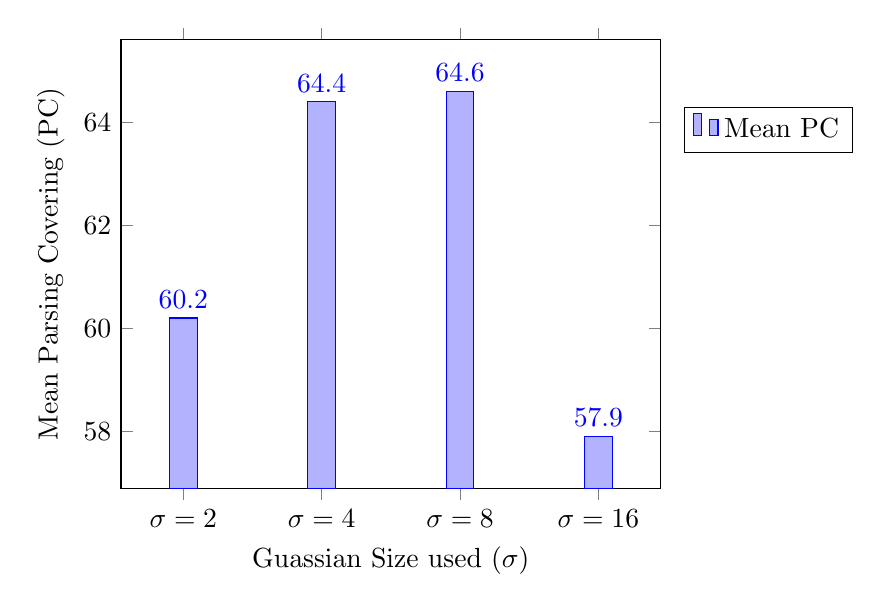
\begin{tikzpicture}  
\begin{axis}  
[      ybar,  
    enlargelimits=0.15,
    legend style={at={(1.2, 0.85)},
    anchor=north,legend columns=-1},
    ylabel={Mean Parsing Covering (PC)}, % the ylabel must precede a # symbol.  
    xlabel={Guassian Size used  $(\sigma)$},  
    symbolic x coords={$\sigma = 2$, $\sigma = 4$, $\sigma = 8$, $\sigma = 16$}, % these are the specification of coordinates on the x-axis.  
    xtick=data,  
     nodes near coords, % this command is used to mention the y-axis points on the top of the particular bar.  
    nodes near coords align={vertical},  
    ]  
\addplot coordinates {($\sigma = 2$,60.2) ($\sigma = 4$,64.4) ($\sigma = 8$,64.6) ($\sigma = 16$,57.9)};  
\legend{Mean PC}
\end{axis}  
\end{tikzpicture} 
\label{fig:bargraph_centerpoints}
\caption[Bar Graph for Gaussian Distribution Size Comparison]{Comparison between models trained on different distribution sizes $(\sigma)$, showing that model trained on guassian with a standard deviation $\sigma=8$ performs best among 4 distribution sizes.}
\end{figure}


Comparison between the above experiments (refer to comparison graph \ref{fig:bargraph_centerpoints}),  suggests that a guassian with a standard deviation $\sigma$ of 8-pixel is most suitable among the compared sizes to encode the center point of pixels for the given dataset which results in mean parsing covering of $\mathbf{64.6}$.

A closer look into the results show very similar overall performance between $\sigma =$ 4 and $\sigma =$ 8 which are $64.4$ and $64.6$ respectively. It can also be observed from table \ref{tab:distribution_comparison} that \textit{rider} and \textit{motorcycle} classes favour a relatively smaller distribution size of $\sigma$ = 4 pixels for the best performance in the given comparison. However \textit{car}, \textit{truck}, \textit{bus} and \textit{train} resulted in a better performance when encoded with a gaussian of standard deviation $\sigma$ = 8.  This is also an interesting find that suggests a smaller distribution size for smaller instances and vice versa. Another important mention here is the fact that not only \textit{things} classes were affected by varying $\sigma$ but it also had an effect on \textit{stuff} classes in particular \textit{pole}, \textit{traffic light} and \textit{traffic sign} showed a better performance when network was trained on a smaller distribution size of $\sigma$ = 4-pixels. It can be argued that smaller distribution size enforced the network to distinguish between classes that have smaller sizes. 



\begin{figure}[!htp] %!ht
%\centering
    \subfigure[Raw Center Prediction at $\sigma = 16-pixels$]{
        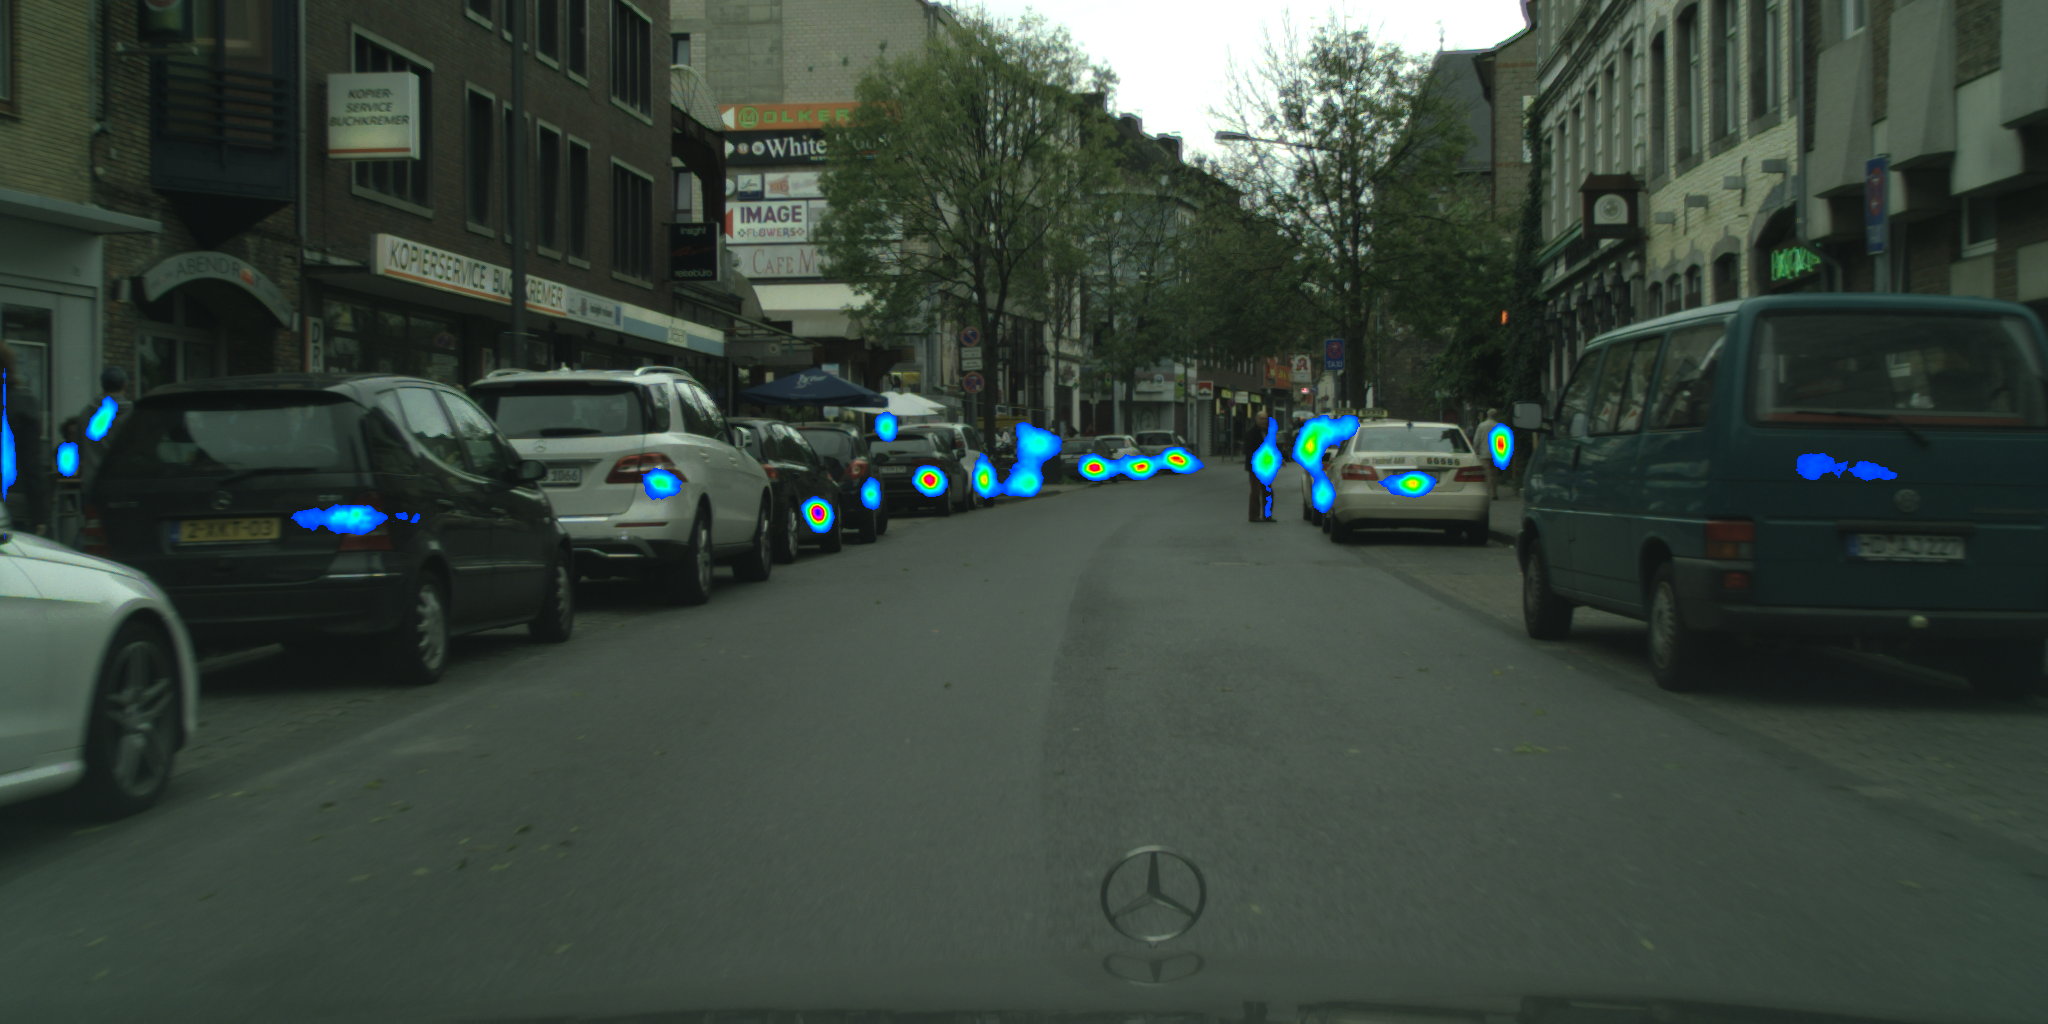
\includegraphics[width = \textwidth / 2 ]{Graphics/Evaluations/Keypoints/000355_prediction33x33}
            \label{fig:K1A}}
    \subfigure[Raw Center Prediction at $\sigma = 2-pixels$]{
        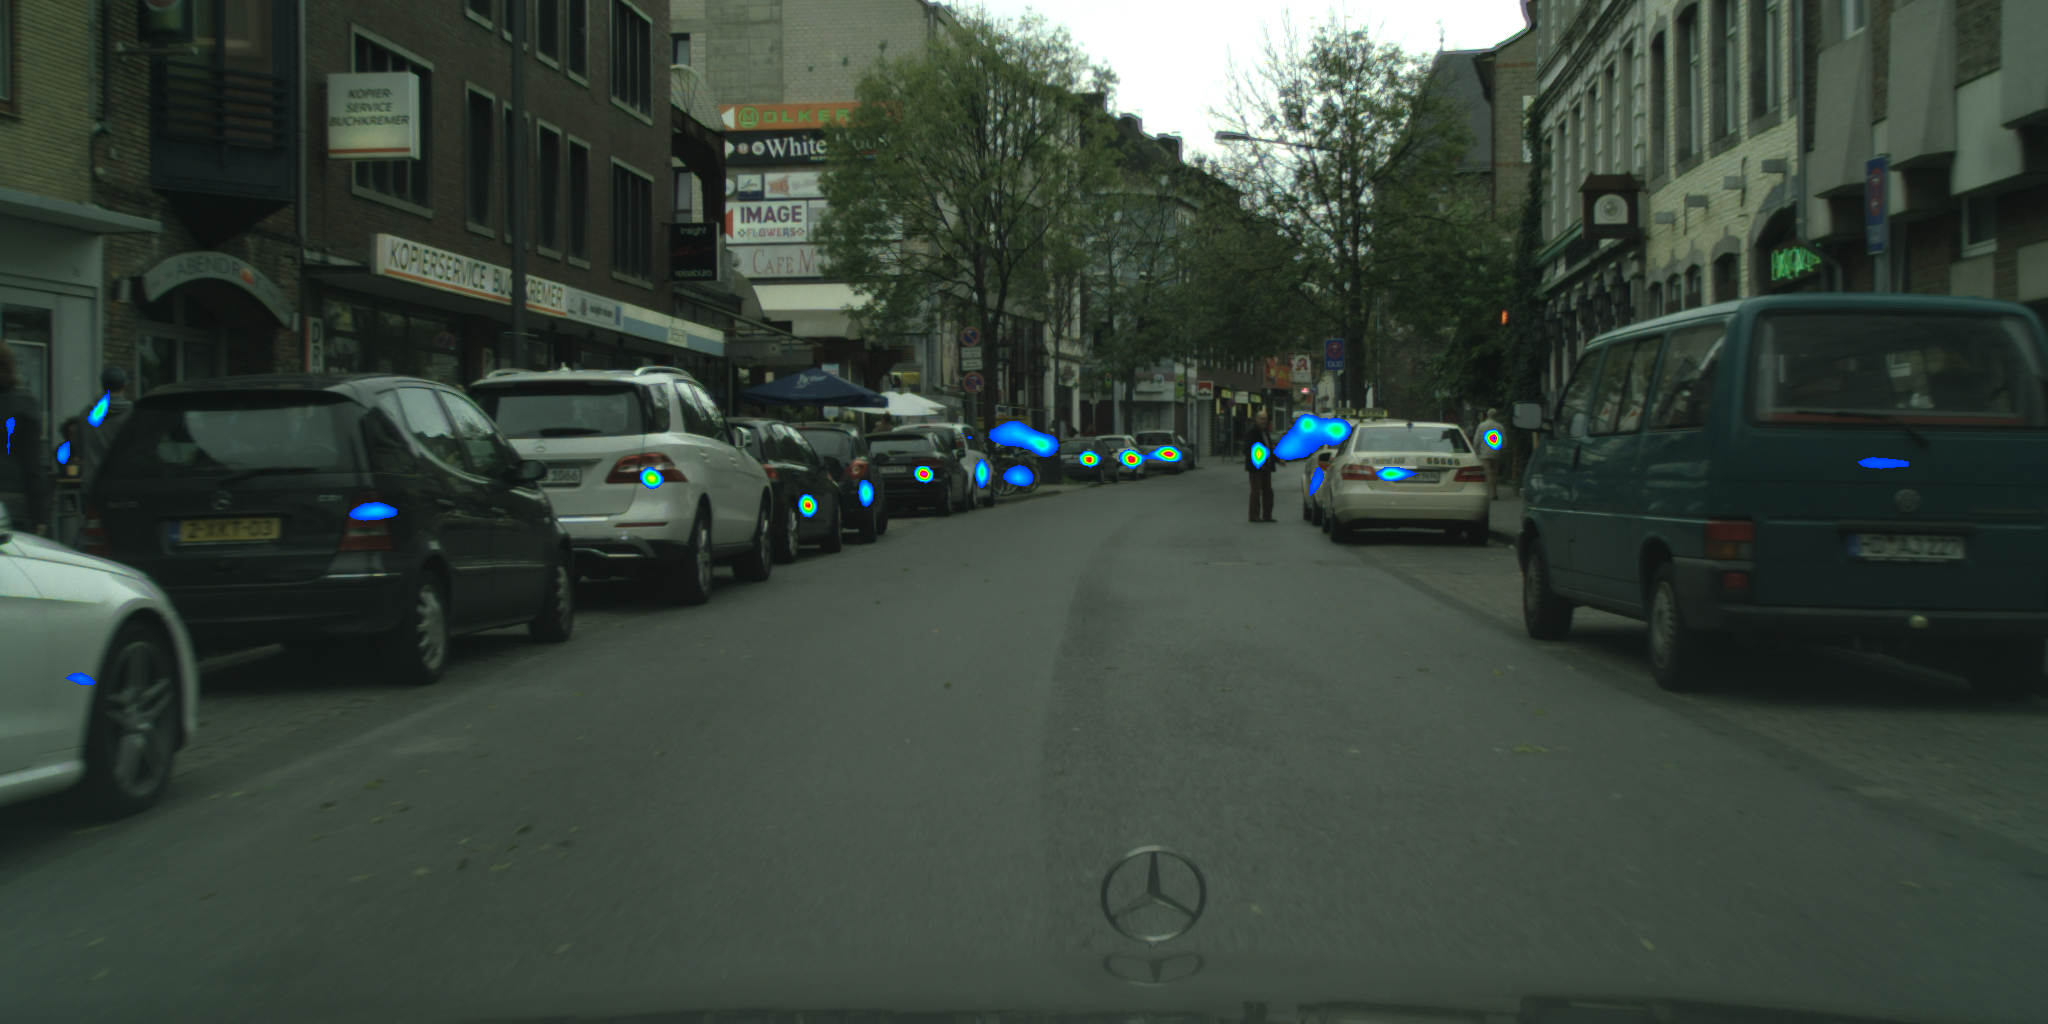
\includegraphics[width = \textwidth / 2 ]{Graphics/Evaluations/Keypoints/000355_prediction}
        \label{fig:K1B}}
    \subfigure[Raw Center Prediction at $\sigma = 16-pixels$]{
        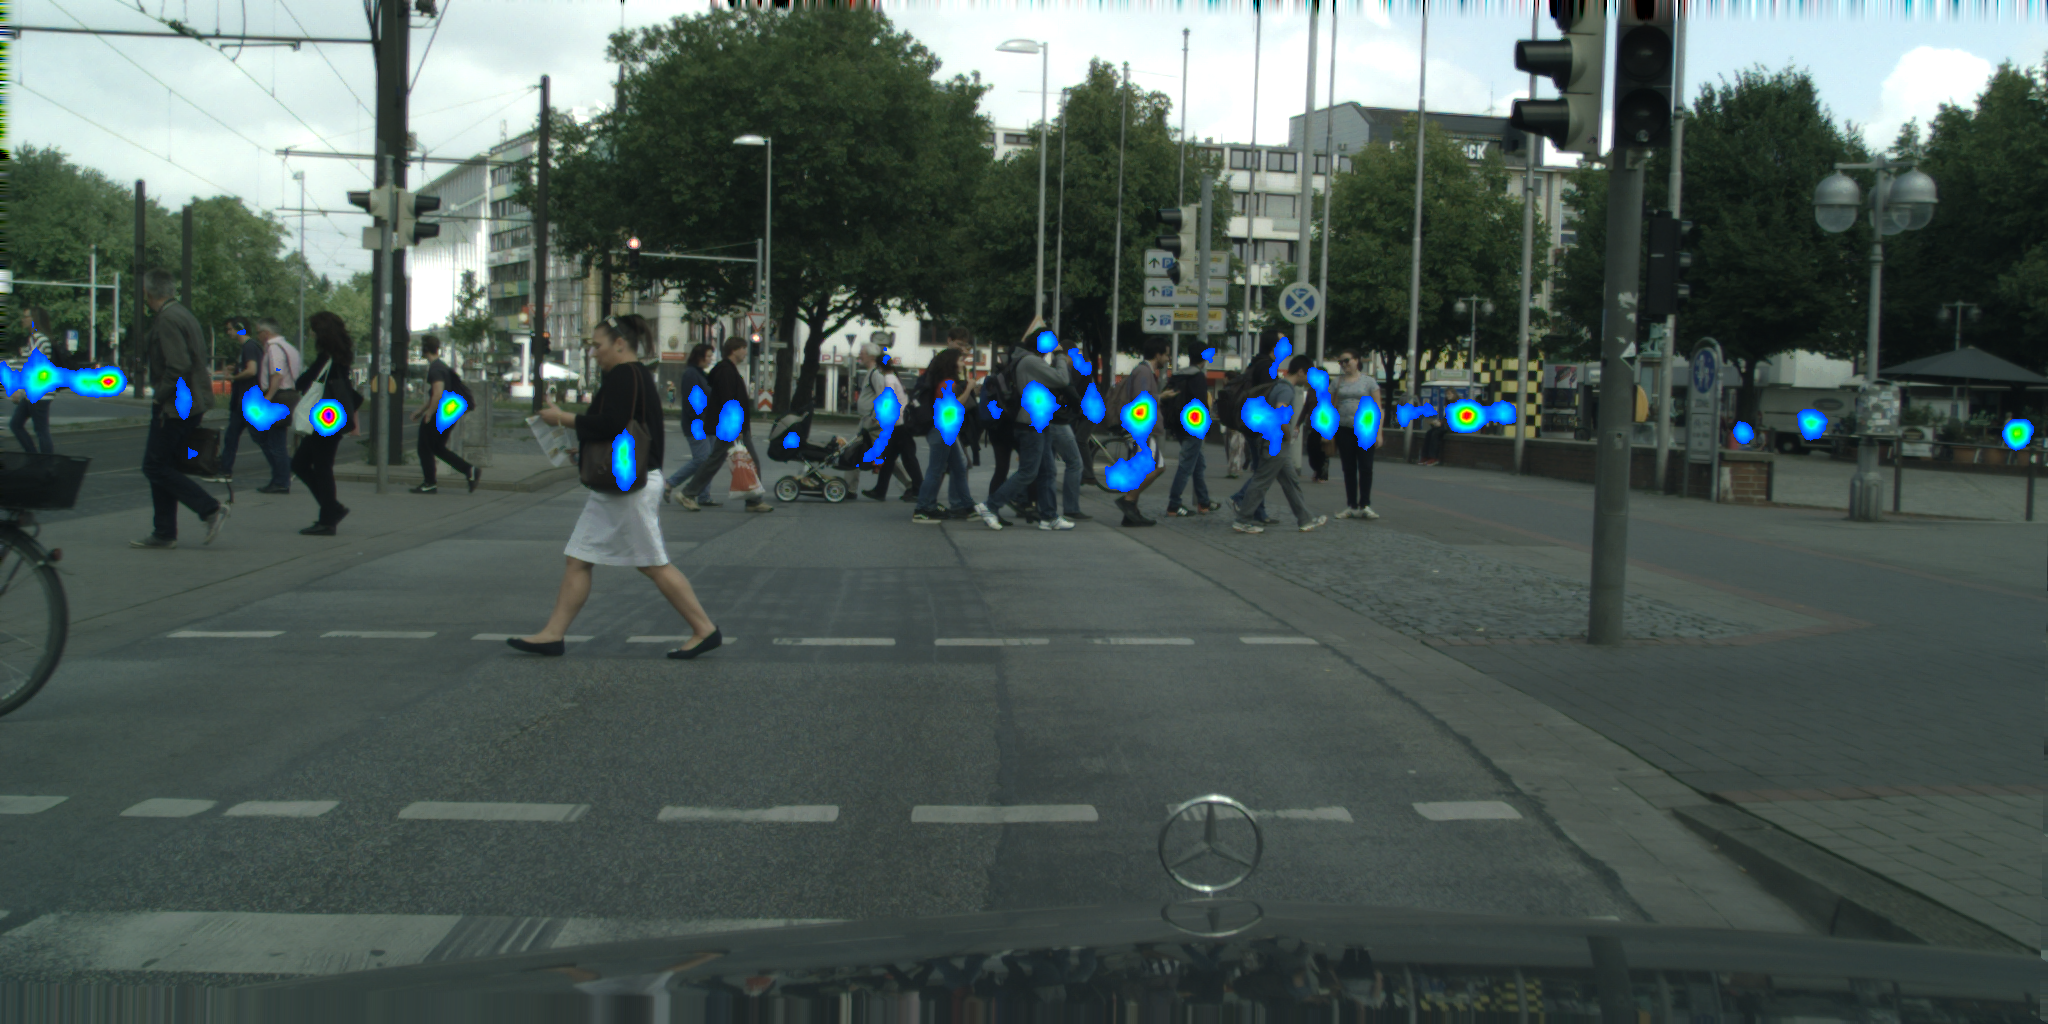
\includegraphics[width = \textwidth / 2 ]{Graphics/Evaluations/Keypoints/000607_prediction}
        \label{fig:K2A}}
    \subfigure[Raw Center Prediction at $\sigma = 2-pixels$]{
        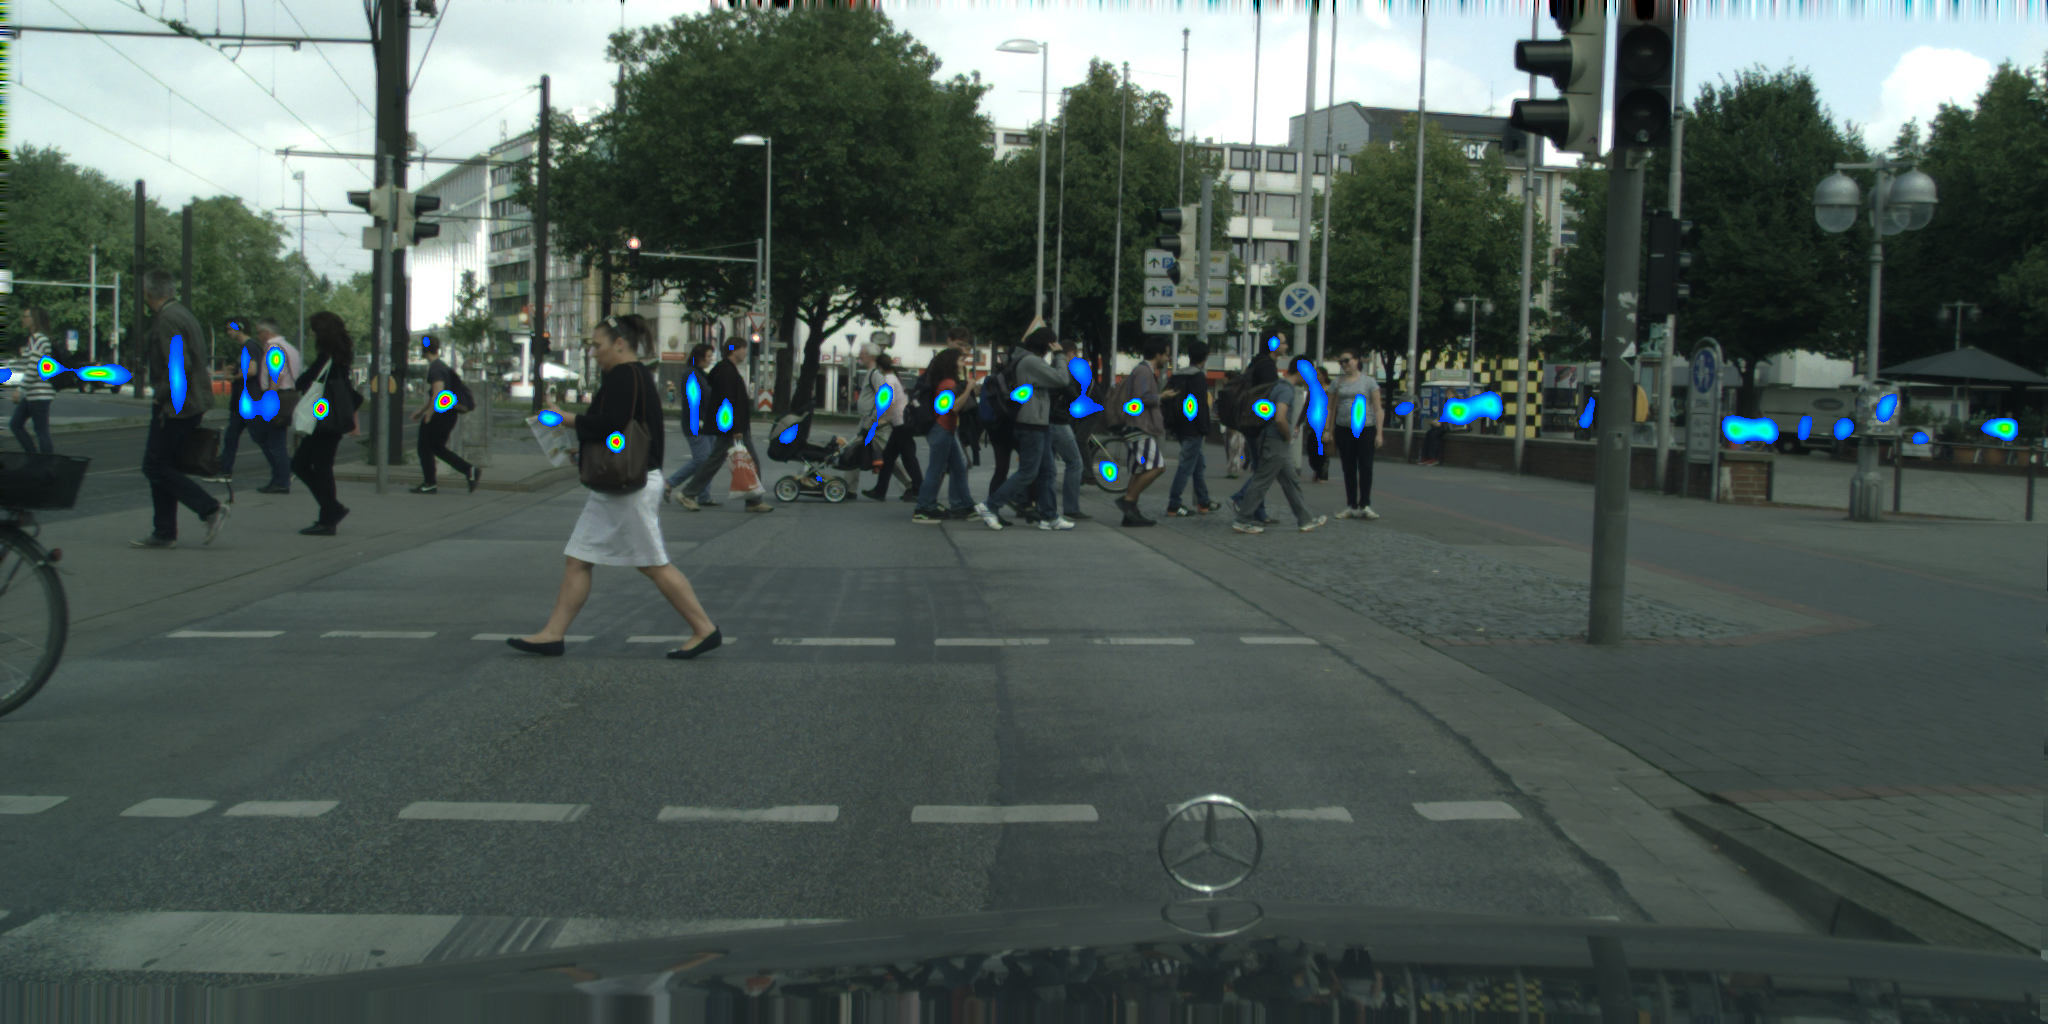
\includegraphics[width = \textwidth / 2 ]{Graphics/Evaluations/Keypoints/000617_prediction}
        \label{fig:K2B}}
    \subfigure[Raw Center Prediction at $\sigma = 16-pixels$]{
        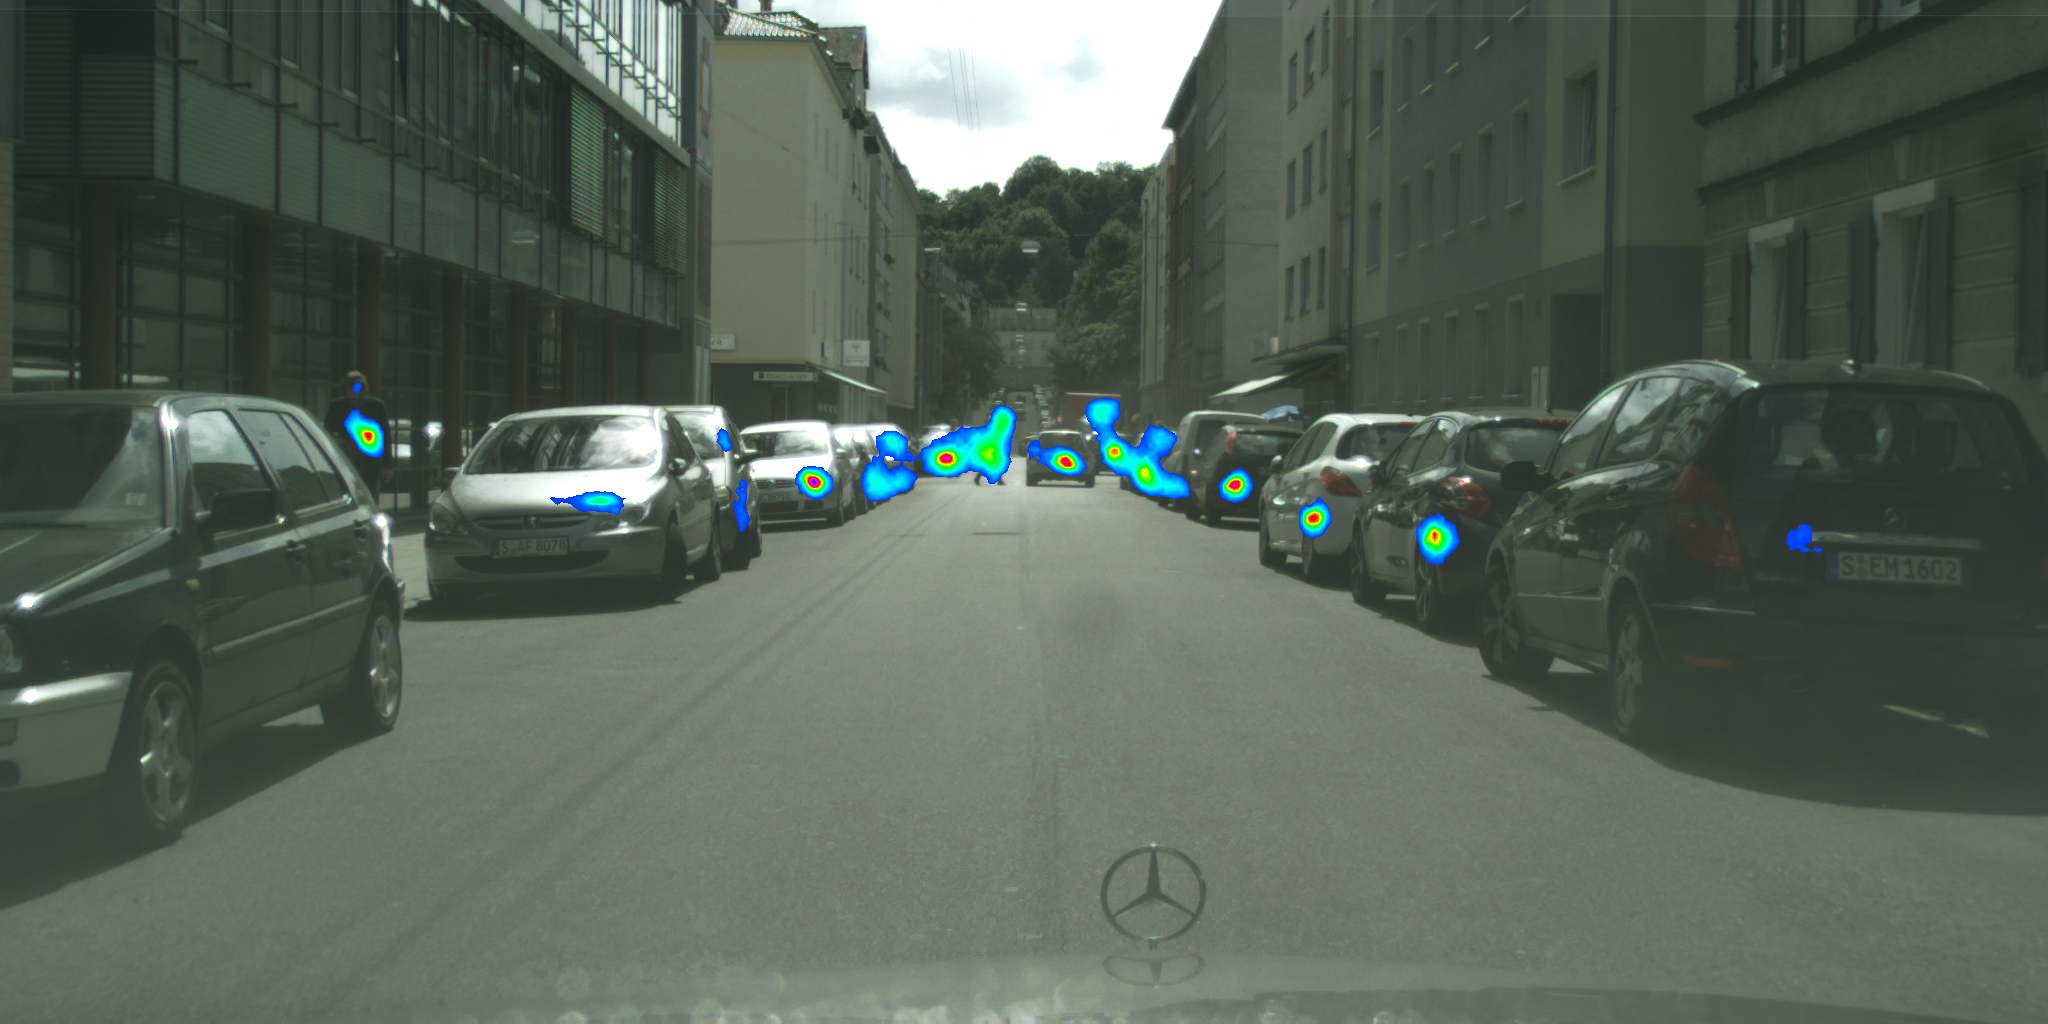
\includegraphics[width = \textwidth / 2 ]{Graphics/Evaluations/Keypoints/000053_prediction}
        \label{fig:K3A}}
    \subfigure[Raw Center Prediction at $\sigma = 2-pixels$]{
        \includegraphics[width = \textwidth / 2 ]{Graphics/Evaluations/Keypoints/000055_prediction}
        \label{fig:K3B}}
    \subfigure[Raw Center Prediction at $\sigma = 16-pixels$]{
        \includegraphics[width = \textwidth / 2 ]{Graphics/Evaluations/Keypoints/000207_prediction.png}
        \label{fig:K4A}}
    \subfigure[Raw Center Prediction at $\sigma = 2-pixels$]{
        \includegraphics[width = \textwidth / 2 ]{Graphics/Evaluations/Keypoints/000208_prediction}
        \label{fig:K4B}}
    \subfigure[Raw Center Prediction at $\sigma = 16-pixels$]{
        \includegraphics[width = \textwidth / 2 ]{Graphics/Evaluations/Keypoints/000234_prediction}
        \label{fig:K5A}}
    \subfigure[Raw Center Prediction at $\sigma = 2-pixels$]{
        \includegraphics[width = \textwidth / 2 ]{Graphics/Evaluations/Keypoints/000234_prediction5x5}
        \label{fig:K5B}}
    \caption[Raw Center Prediction Comparison] {Qualitative Comparison of predictions from models trained on different distribution sizes. Left column shows the output from model trained on center-points encoded with a guassian of standard deviation ($\sigma$) - 16 pixels. Whereas, right column shows the predicted output from model trained on center-points encoded with a guassian of standard deviation ($\sigma$) - 2 pixels. }
    \label{fig:Keypoints_comparison}
\end{figure}



For further analytical observation and reasoning, figure \ref{fig:Keypoints_comparison} illustrates a comparison between predicted center-points from two models where left column shows the output from model trained on center-points encoded with a guassian of standard deviation ($\sigma$) - 16 pixels. Whereas, right column shows the predicted output from model trained on center-points encoded with a guassian of standard deviation ($\sigma$) - 2 pixels. Models trained with two extreme sizes are chosen for qualitative comparison to highlight the differences. It can be seen that predictions on the right column are precise in terms of center localization i.e. predictions suggest comparatively smaller region for each predicted center point thus more precise in locating center points. Another observation that can be made from the illustrated images is the fact that center points shown on the right column are not only precise in term of space but also exhibit a relatively higher confidence for each center point.

Although a larger distribution size might seem to have greater influence on training and might lead to a faster convergence in some cases, following two important observations can be made by comparing corresponding predicted outputs.

\begin{enumerate}
    \item Comparatively smaller distribution size improve spatial precision. 
    \item Encoding with a larger distribution degrades prediction confidence.
\end{enumerate}

Therefore, it is important to consider right distribution size choice for respective domain.
%For the scope of presented work, experiments suggest a center-point encoding with $\sigma = 8$ pixels to be appropriate.


\section{Offset-Encoding Comparison}


In this section, offset encodings introduced in chapter \ref{sec:data_representation} are evaluated.
Offset representations basically encode distance to center for each instance. Since, offset values predicted by network are used to group pixels to generate class-agnostic instance segmentation, it is therefore important that these representations are effective and are structured in a way that are efficiently learned by the network. To this end, various experiments have been carried out to study these representations both qualitatively and quantitatively. For legibility, instead of providing class-level details, table \ref{tab:encodings_table} lists \textit{ mean parsing covering} over things and stuff classes individually as well as an overall mean parsing covering (Mean PC) over all classes.

\sisetup{round-mode = places, round-precision = 1, scientific-notation = fixed, fixed-exponent = 0}
\begin{table}[!htbp]
    \centering
    \begin{tabular}{crSSS}
        \hline
        & & $\mathbf{PC_{Stuff}}$ & $\mathbf{PC_{Things}}$ & $\mathbf{PC_{Mean}}$\\%
        \hline
        \parbox[t]{2mm}{\multirow{4}{*}{\rotatebox[origin=c]{90}{$Encoding$}}}
        & $\mathbf{End-End_{8}}$ & 72.9 & 54.1 & 65.0 \\
        & $\mathbf{Center-End_{8}}$ & 72.045 & 54.35 & 64.6 \\
        & $\mathbf{End-End_{16}}$ & 65.3 & 52.9 & 60.1 \\
        & $\mathbf{Center-End_{16}}$ & 67.2 & 45.15 & 57.9 \\
        \hline
    \end{tabular}
    \caption[Evaluation of Encoding Types ]{Comparison of center-end encoding and end-end encoding with trained in combination with center-points encoded as gaussian of standard deviation ($\sigma$) 8 and 16 pixels.}
    \label{tab:encodings_table}
\end{table}

In the table \ref{tab:encodings_table}, rows represent encoding type, whereas the number in the subscript of each element represents the encoding size used for training center points. From table above, it is evident that best parsing covering results have been achieved using center-points of standard deviation 8 pixels. Mean parsing covering  of $65.0$ has been achieved with end-to-end encoding, while the center-to-end encoding with same distribution size resulted in mean parsing covering of $64.6$. This again validates the results from previous section about the center point size. Furthermore, it also appears from the results in table \ref{tab:encodings_table} that end-end encoding is preferred encoding style, however this might not always be the case. Figure \ref{fig:Encodings_comparison}, provides few sample outputs generated using end-end encoding and center-end encoding. The column on the left shows outputs generated using end-end encoding while the right column shows corresponding images generated using center-end encoding. Since, outputs in the left column are generated using end-end encoding where network was expected to predict offset magnitude and direction with respect to center, it appeared to be relatively ambiguous for post-processing step to delineate boundaries between different instances. However, it can also be seen that number of masks generated in end-end cases are almost right but sense of instance boundaries is not retained. On the other hand, instance masks generated using predictions from the model trained on center-end encoding resulted in much better boundary separations which is evident from the figure \ref{fig:Encodings_comparison} - right column.

It has been observed that this happens due to the following reasons:

\begin{enumerate}
    \item Representation learned by the network is simpler i.e just distance to the center.
    \item Explicitly inverting offsets in center-end encoding gives larger separation across neighbouring instances, see figure \ref{fig:c2e_vis_pixels}.
\end{enumerate}


A more detailed class-wise parsing covering has been documented in the table \ref{tab:encoding_comparisonclass-wise} 

\begin{table}[!htp]
  \resizebox{1 \textwidth}{!}{
  \begin{tabular}{@{}rcccccccccccccccccccc@{}}

  & \multicolumn{1}{P{90}{1.6cm}}{Road} &
    \multicolumn{1}{P{90}{1.6cm}}{Sidewalk} &
    \multicolumn{1}{P{90}{1.6cm}@{}}{Building} &
    \multicolumn{1}{P{90}{1.6cm}}{Wall} &
    \multicolumn{1}{P{90}{1.6cm}}{Fence} &
    \multicolumn{1}{P{90}{1.6cm}@{}}{Pole} &
    \multicolumn{1}{P{90}{1.6cm}}{Traffic Light} &
    \multicolumn{1}{P{90}{1.6cm}}{Traffic Sign} &
    \multicolumn{1}{P{90}{1.6cm}@{}}{Vegetation} &
    \multicolumn{1}{P{90}{1.6cm}}{Terrain} &
    \multicolumn{1}{P{90}{1.6cm}}{Sky} &
    \multicolumn{1}{P{90}{1.6cm}@{}}{Person} &
    \multicolumn{1}{P{90}{1.6cm}}{Rider} &
    \multicolumn{1}{P{90}{1.6cm}}{Car} &
    \multicolumn{1}{P{90}{1.6cm}@{}}{Truck}&
    \multicolumn{1}{P{90}{1.6cm}}{Bus} &
    \multicolumn{1}{P{90}{1.6cm}@{}}{Train} &
    \multicolumn{1}{P{90}{1.6cm}}{Motorcycle} &
    \multicolumn{1}{P{90}{1.6cm}}{Bicycle} &
    \multicolumn{1}{P{90}{1.6cm}@{}}{\textbf{Mean}}\\
      \midrule
        $\mathbf{End-End_{8}}$ 
        &97.7&83.0&90.7&52.4&57.1&51.1&56.2&67.5&91.0&61.7&93.9&44.9&42.2&63.9&68.6&64.1&59.0&53.8&46.1&\texbf{65.0} \\
        
        $\mathbf{Center-End_{8}}$
        &97.7&83.6&90.3&52.9&53.7&48.7&54.3&66.2&90.7&61.3&93.1&45.2&41.2&64.3&73.3&65.0&66.7&40.9&38.2&\textbf{64.6} \\
        
        $\mathbf{End-End_{16}}$ 
        &96.0&75.0&87.4&43.6&52.8&31.1&42.7&54.4&87.2&58.4&89.7&39.4&38.6&61.7&72.9&61.8&62.1&43.7&43.3&\textbf{60.1} \\
        
        $\mathbf{Center-End_{16}}$ &96.2&76.1&88.1&44.7&49.3&35.5&50.4&58.2&89.1&60.18&91.6&43.8&37.5&59.9&63.5&52.6&30.1&37.8&36.0&\textbf{57.9} \\
     
     \bottomrule
  \end{tabular}
  }
  \caption[Comparison of Encoding types]{Comparison of center-end encoding and end-end encoding trained in combination with center-points encoded as gaussian of standard deviation ($\sigma$) 8 and 16 pixels as shown in the subscript.}
  \label{tab:encoding_comparisonclass-wise}
\end{table}




Table \ref{fig:Encodings_comparison} shows class-wise parsing covering for all the classes including both \textit{things} and \textit{stuff} classes. Here again \textit{End-End} and \textit{Center-End} represent encoding types and the number in the subscript shows the corresponding center point distribution chosen to train the network. For a better comparison two pairs of networks have been shown. It has been observed that \gls{pc} for stuff classes remains almost the same for models irrespective of the encoding type except for the models that have been trained with a gaussian distribution of $\sigma$ = 16 which has been shown in the table. Another interesting observation that can be made from the experiment results is the fact that \textit{rider}, \textit{motorcycle} and \textit{bicycle} show a better performance when trained with end to end encoding however \textit{person} and other larger \textit{things} classes show an improved performance when trained on a center-end representation. However a generally better quantitative performance has been achieved by \textit{End-End} encoding due to the fact that \textit{bicycles} and \textit{motorcycle} have shown to have $7.9\%$ and $12.9\%$  improvement when learned with End-End encoding.  Therefore End-End encoding results in better suited encoding for two-wheeled instances in comparison to Center-End encoding.


\begin{figure}[H] %!ht
%\centering
    \subfigure[End to End Encoding Result]{
        \includegraphics[width = \textwidth / 2 ]{Graphics/Evaluations/OffsetVectos/000689_prediction}
            \label{fig:O1A}}
    \subfigure[Center to End Encoding Result]{
        \includegraphics[width = \textwidth / 2 ]{Graphics/Evaluations/OffsetVectos/000686_prediction}
        \label{fig:O1B}}
    \subfigure[End to End Encoding Result]{
        \includegraphics[width = \textwidth / 2 ]{Graphics/Evaluations/OffsetVectos/001452_prediction}
        \label{fig:O2A}}
%   \hspace{1pt}
    \subfigure[Center to End Encoding Result]{
        \includegraphics[width = \textwidth / 2 ]{Graphics/Evaluations/OffsetVectos/001447_prediction}
        \label{fig:O2B}}
    \subfigure[End to End Encoding Result]{
        \includegraphics[width = \textwidth / 2 ]{Graphics/Evaluations/OffsetVectos/000686_pred4iction}
        \label{fig:O3A}}
    \subfigure[Center to End Encoding Result]{
        \includegraphics[width = \textwidth / 2 ]{Graphics/Evaluations/OffsetVectos/000684_prediction}
        \label{fig:O3B}}
    \subfigure[End to End Encoding Result]{
        \includegraphics[width = \textwidth / 2 ]{Graphics/Evaluations/OffsetVectos/000418_prediction}
        \label{fig:O4A}}
%   \hspace{1pt}
    \subfigure[Center to End Encoding Result]{
        \includegraphics[width = \textwidth / 2 ]{Graphics/Evaluations/OffsetVectos/000415_prediction}
        \label{fig:O4B}}
        \subfigure[End to End Encoding Result]{
        \includegraphics[width = \textwidth / 2 ]{Graphics/Evaluations/OffsetVectos/001733_prediction}
        \label{fig:O5A}}
%   \hspace{1pt}
    \subfigure[Center to End Encoding Result]{
        \includegraphics[width = \textwidth / 2 ]{Graphics/Evaluations/OffsetVectos/001732_prediction}
        \label{fig:O5B}}
    \caption[Qualitative Comparison of Encodings] {Qualitative comparison of instance segmentation masks generated using end-end encoding and center-end encoding. Left column shows instance mask generated using prediction from model that was trained on end-end encoding while the right column presents the instance segmentation generated using predictions from model, trained on center-end encoding}
    \label{fig:Encodings_comparison}
\end{figure}


\section{Post-processing Parameter Comparison}
\label{subsec:post-processingparameters}

Outputs generated by presented panoptic segmentation network is post-processed to generate instance segmentation out of center point prediction and offset predictions. Raw center predictions are essentially probability distributions around perspective center points. First step in generating instance segmentation from the aforementioned representations is to get exact center locations from predicted center distribution output. To achieve that a hard threshold is applied to the center predictions which is subsequently followed by a max-pooling based non-maxima suppression \gls{nms} operation that pools the pixel with highest predicted probability in each pooling window, thus extracting center positions from predicted distributions. For more details, reader is referred to \ref{subsec:center_rendering}.

Pooling right number of center points is critical for generating a representation with least false positives and false negatives. To this end, several experiments were performed to choose :

\begin{itemize}
    \item  Threshold value.
    \item  Pooling window size.
\end{itemize}

A coarse grid-search was made to study the affects of these parameters on overall panoptic segmentation task. Comparison of these parameters with respect to mean parsing covering has been compared in plot \ref{plot:post-processingcomparison}, see also table \ref{tab:parameter_comparison} for comparison.

\begin{figure}[h]{

\centering
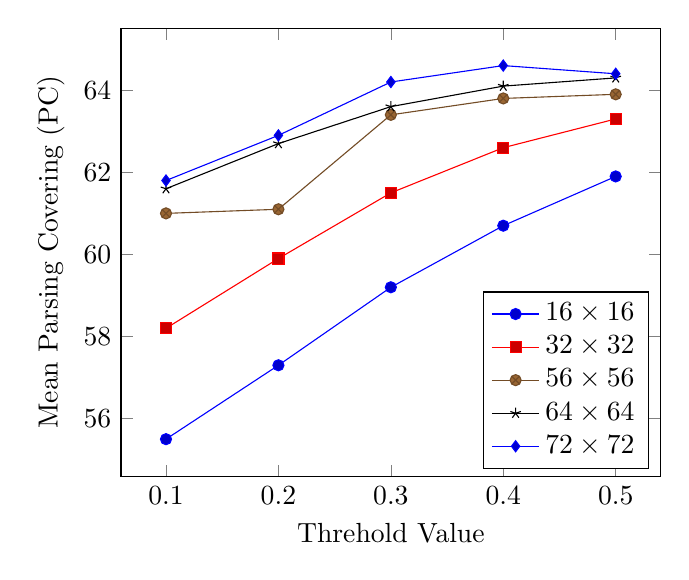
\begin{tikzpicture}
    \begin{axis}[
        xlabel=Threhold Value,
        ylabel=Mean Parsing Covering (PC),
        legend style={at={(0.67,0.215)},anchor=west}]
    \addplot plot coordinates {
        (0.1, 55.5)
        (0.2, 57.3)
        (0.3, 59.2)
        (0.4, 60.7)
        (0.5, 61.9)
    };
    \addlegendentry{$16\times16$}
    
    \addplot plot coordinates {
        (0.1, 58.2)
        (0.2, 59.9)
        (0.3, 61.5)
        (0.4, 62.6)
        (0.5, 63.3)
    };
    \addlegendentry{$32\times32$}
    
    \addplot plot coordinates {
        (0.1, 61.0)
        (0.2, 61.1)
        (0.3, 63.4)
        (0.4, 63.8)
        (0.5, 63.9)
    };
    \addlegendentry{$56\times56$}
    
    \addplot plot coordinates {
        (0.1, 61.6)
        (0.2, 62.7)
        (0.3, 63.6)
        (0.4, 64.1)
        (0.5, 64.3)
    };
    \addlegendentry{$64\times64$}
    
    \addplot plot coordinates {
        (0.1, 61.8)
        (0.2, 62.9)
        (0.3, 64.2)
        (0.4, 64.6)
        (0.5, 64.4)
    };
    \addlegendentry{$72\times72$}


    \end{axis}
\end{tikzpicture}
\label{plot:post-processingcomparison}
\caption[Post-processing Parameters Comparison ]{Comparison plot for parsing covering \gls{pc} at multiple threshold values and kernel window sizes showing a threshold value of around 0.4 and a pooling window of size $72\times72$ to be a favourable parameter choice.}}
\end{figure}

Further quantitative results corresponding to each investigated thershold level and kernel window for pooling center points has been illustrated in the table \ref{tab:parameter_comparison} below.

\sisetup{round-mode = places, round-precision = 1, scientific-notation = fixed, fixed-exponent = 0}
\begin{table}[H] % !htbp
    \centering
    \begin{tabular}{crSSSSS}
        \hline
        & & $Th_{0.1}$ & $Th_{0.2}$ & $Th_{0.3}$ & $Th_{0.4}$& $Th_{0.5}$ \\%
        \hline
        \parbox[t]{2mm}{\multirow{4}{*}{\rotatebox[origin=c]{90}{Kernel Size  }}}
        & $\mathbf{16\times16}$ & 55.5 & 57.3 & 59.2 & 60.7 & 61.9 \\
        & $\mathbf{32\times32}$ & 58.2 & 59.9 & 61.5 & 62.6 & 63.25\\
        & $\mathbf{56\times56}$ & 61.02 & 61.08 & 63.4 & 63.8 & 63.9\\
        & $\mathbf{64\times64}$ & 61.6 & 62.7 & 63.6 & 64.1 & 64.3\\
        & $\mathbf{72\times72}$ & 61.8 & 62.9 & 64.2 & \textbf{64.6} & 64.4\\
        \hline
    \end{tabular}
    \caption[Comparison of Threshold value and Pooling Kernel Window]{Table provides a comparison between various threshold values and pooling kernel window size. It can be seen that threshold of about 0.4 and pooling kernel of $72\times72$ results in best performance}
    \label{tab:parameter_comparison}
\end{table}


Comparison shows a threshold value of around 0.4 and a pooling window size of $72\times72$ to be a favourable parameter choice. Therefore, these parameters have been chosen as default for further experimentation at an early stage of evaluation.



\section{Overall Panoptic Task Evaluation}

Lessons learned from experiments with post-processing parameters have been used to select best performing settings. These parameters have been fixed for further experimentation and evaluation purposes. Therefore, a comparison after selecting these parameters has been provided in this section. Table \ref{tab:PC_overall} shows a comparison of different encoding types and center point distribution sizes with respect to class-wise parsing covering. \textit{End-End} and \textit{Center-End} represent encoding type while the number in subscript represents the distribution size used to encode the center-points.



\begin{table}[!htp] % 
  \resizebox{1 \textwidth}{!}{
  \begin{tabular}{@{}rcccccccccccccccccccc@{}}

  & \multicolumn{1}{P{90}{1.6cm}}{Road} &
    \multicolumn{1}{P{90}{1.6cm}}{Sidewalk} &
    \multicolumn{1}{P{90}{1.6cm}@{}}{Building} &
    \multicolumn{1}{P{90}{1.6cm}}{Wall} &
    \multicolumn{1}{P{90}{1.6cm}}{Fence} &
    \multicolumn{1}{P{90}{1.6cm}@{}}{Pole} &
    \multicolumn{1}{P{90}{1.6cm}}{Traffic Light} &
    \multicolumn{1}{P{90}{1.6cm}}{Traffic Sign} &
    \multicolumn{1}{P{90}{1.6cm}@{}}{Vegetation} &
    \multicolumn{1}{P{90}{1.6cm}}{Terrain} &
    \multicolumn{1}{P{90}{1.6cm}}{Sky} &
    \multicolumn{1}{P{90}{1.6cm}@{}}{Person} &
    \multicolumn{1}{P{90}{1.6cm}}{Rider} &
    \multicolumn{1}{P{90}{1.6cm}}{Car} &
    \multicolumn{1}{P{90}{1.6cm}@{}}{Truck}&
    \multicolumn{1}{P{90}{1.6cm}}{Bus} &
    \multicolumn{1}{P{90}{1.6cm}@{}}{Train} &
    \multicolumn{1}{P{90}{1.6cm}}{Motorcycle} &
    \multicolumn{1}{P{90}{1.6cm}}{Bicycle} &
    \multicolumn{1}{P{90}{1.6cm}@{}}{ \textbf{Mean}}\\
      \midrule

        $\mathbf{End-End_{8}}$ 
        &97.7&83.0&90.7&52.4&57.1&51.1&56.2&67.5&91.0&61.7&93.9&44.9&42.2&63.9&68.6&64.1&59.0&53.8&46.1&\texbf{65.0} \\
        
        $\mathbf{End-End_{16}}$ &96.0&75.0&87.4&43.6&52.8&31.1&42.7&54.4&87.2&58.4&89.7&39.4&38.6&61.7&72.9&61.8&62.1&43.7&43.3&60.1 \\
        $\mathbf{Center-End_{2}}$ &97.6&82.4&90.0&50.0&55.9&42.8&56.5&63.9&90.3&63.23&93.0&39.0&41.5&55.8&69.7&46.9&29.1&39.6&36.1&60.2 \\
        $\mathbf{Center-End_{4}}$ &97.8&83.7&90.8&52.8&54.6&50.7&59.3&68.2&91.1&63.3&93.9&42.7&43.4&61.1&66.1&61.2&64.1&42.0&36.7&64.4  \\
        $\mathbf{Center-End_{8}}$ &97.7 &83.6&90.3&52.9&53.7&48.7&54.3&66.2&90.7&61.3&93.1&45.2&41.2&64.3&73.3&65.0&66.7&40.9&38.2&\textbf{64.6} \\
        $\mathbf{Center-End_{16}}$ &96.2&76.1&88.1&44.7&49.3&35.5&50.4&58.2&89.1&60.18&91.6&43.8&37.5&59.9&63.5&52.6&30.1&37.8&36.0&57.9 \\

  \bottomrule
  \end{tabular}
  }
\caption[Overall Panoptic Task Comparison]{Comparison of different encoding types and center point distribution sizes with respect to class-wise parsing covering. Names \textit{End-End} and \textit{Center-End} represent encoding type while the number in subscript represents the distribution size used to encode the center-points.}
  \label{tab:PC_overall}
\end{table}

Comparison result suggest an appropriate size for encodings of different sizes. In general, it can be seen that smaller instances such as \textit{rider}, \textit{motorcycle} show a better performance when encoded with a smaller distribution sizes. However instances that are larger in size such as \textit{car}, \textit{truck}, \textit{bus} and \textit{train} favour a larger distribution size to encode center points. An overall best performance has been shown by encoding all the instances with a center point encoded using a guassian of standard deviation $\sigma$ = 8 pixels. 

\paragraph{Comparison with the State-of-the-Art}

Table \ref{tab:sotacomparison} shows a comparison between proposed models with xception-65 as backbone feature extractor trained on input size of $1025 \times 1025$ and batch-size = 1 with state of the art DeeperLab \cite{DBLPDeeperLab:journals/corr/abs-1902-05093}. Reported metric is \gls{pc} which is a newly proposed metric for quantifying panpotic segmentation therefore not alot of approaches have yet reported parsing covering for the evaluation of their approaches. It can be seen that proposed models with center-to-end and end-to-end encoding show a comparable performance even with smaller train crop size, partial cold start of training and a train batch size of 1 due to limited computational resources. Note that model from deeperlab uses full image resolution and manifold batch size.  
 
\begin{table}[H]
    \centering
        \begin{tabular}{cc|c} 
        \hline
            Method & Input Size  & PC $(\%)$ \\
            \hline DeeperLab - MNV2 & $513 \times 1025$  &64.66 \\
            DeeperLab - MNV2 & $1025 \times 2049$ &69.70 \\
            DeeperLab - Xception-71 &$1025 \times 2049$ &75.63 \\
            \hline (Ours) Xception-65_{c2e} &$1025 \times 1025$ &\texbf{64.6} \\
            (Ours) Xception-65_{e2e} & $1025 \times 1025$ &\texbf{65.0} \\
            \hline
        \end{tabular}
    \caption[Comparison with State of the art]{Comparison with state of the art DeeperLab with presented models at different input training sizes.}
    \label{tab:sotacomparison}
\end{table}



\section{Limitation}

Generating instance masks from center-points and offset vector representation has been employed as a simple regression problem, see section \ref{subsec:regression_approach}. Before such a grouping operation can initiate, a simple max-pooling based non-maxima suppression has been employed to get exact center locations, for more details, reader is referred to \ref{subsec:center_rendering}. It is sometimes observed that more than one mask covers a single instance. 
This behaviour has been shown in the figure \ref{fig:failurecaseexamples}

Reason for such behaviour can be explained by following reason:

\begin{enumerate}
    \item Centers predicted by the network are so dispersed that they occur in two consecutive pooling strides
    \item Center predictions occurred at the intersection of consecutive pooling filter strides.
\end{enumerate}

Illustrations of such behaviour has been visualised in the figure \ref{fig:faliurecasereason}.

\begin{figure}[H] %!htp
%\centering
    \subfigure[Failure Case 1]{
        \includegraphics[width = \textwidth / 2 ]{Graphics/Evaluations/failurecase1.png}
        \label{fig:failurecase1}}
    %\hspace{1pt}
     %add desired spacing between images, e. g. ~, \quad, \qquad, \hfill etc.
     %(or a blank line to force the subfigure onto a new line)
    \subfigure[Failure Case 2]{
        \includegraphics[width = \textwidth / 2 ]{Graphics/Evaluations/failurecase2.png}
        \label{fig:failurecase2}}
    \caption[Dual Center Pooling Illustration] {Illustration of center pooling limitation a) depicts an image showing two masks covering single instance on the left on image b) shows a small instance covered by two masks representing two center points pooled from same distribution }
    \label{fig:failurecaseexamples}
\end{figure}



\begin{figure}[H] %!htp
    \includegraphics[width = \textwidth]{Graphics/Evaluations/failurecase_reason}
    \caption[Dual Pooling of Distributions]{Illustration of two centers being pooled from one predicted distribution. Figure showing dispersed predicted distribution being pooled twice in consecutive pooling strides on the left and predicted distribution occurring at intersection of two consecutive pooling kernel strides.}
    \label{fig:faliurecasereason}
\end{figure}
\newpage
\section{Inference Times}


This section provides comparison between different backbone feature extractors against their inference times. 

Since, the feature extractor used for implementation of presented bottom-up panoptic segmentation network architecture relies on feature extractor from state of the art semantic segmentation architecture, it therefore has the possibility to use multiple backbones. Presented network architecture therefore can make use of multiple backbones depending on requirement for accuracy vs speed. It is also possible to manually reduce the maximum number of instances for segmentation by only picking the top-50 or top-200 highest predicted center-points. Therefore, table shows the inference times for both variants. 

\begin{table}[!htp]
\begin{center}

\centering



\begin{tabular}{c|c|c} 
\hline
    Backbone & Upto 200 Instances (msec)&  Upto 50 Instances (msec) \\
    \hline Xception 71 & $389$ & $281$ \\
     Xception 65 & $386$ & $263$ \\
    Xception 41 & $310$ & $191$ \\
    MobileNetv3 Large & $281$ & $162$ \\
    MobileNetv3 Small & $194$ & $102$ \\
    \hline
\end{tabular}
\end{center}
\caption[Comparison of Inference Time with Backbones]{Comparison of inference times in milliseconds incurred by different backbones for 50 and 200 instances.}
\end{table}

Reported inference times for different backbones have been recorded uisng NVIDIA RTX 2080Ti GPU.





% !TeX root = ../thesis.tex

\chapter{Conclusion and  Outlook}
\label{sec:conclusion_future-work}


\section{Conclusion}

The goal of this thesis was to approach panoptic segmentation as multi-task learning problem whereby learning semantic and instance segmentation jointly and presenting a coherent single view representation unifying semantic segmentation for \textit{stuff} classes and instance segmentation for \textit{things} classes. Presented works explored bottom-up paradigm for panoptic segmentation by conceiving and learning on pixel-level relationships to generate instance representations and subsequently instance segmentation. Since it is desired to replace two-stage object detector based approaches for instance segmentation, presented work studies various instance encoding possibilities in greater detail. A general approach adopted for this purpose is representing instances by their center points as reference along with additional modality that encodes pixel-level distances i.e. offset to center points. To this end, various center points and offset representations have been curated and studied. Research on these representations suggest a favourable size for encoding center point can lead to a better performance. It has also been shown that directly learning the offset representations can be tedious however learning a simple representation while leveraging a brief post-processing step can greatly improve instance boundary delineations and thus better instance segmentation results. Therefore, presented work shows a reasonable performance on panoptic segmentation task whilst avoiding top-down and two-stage instance segmentation approaches. It further highlights the importance for selecting a suitable distribution size for encoding key-points. It also provides a detailed comparison between different encoding styles that can be employed for learning offset vectors. 


\section{Future Work}

It has been observed that center of mass used for selecting the center points for instance representations is robust and generally tackles occlusions to a great extent. However, traffic participants such as bicycles and motorbikes are at times get predicted twice due to larger circular wheels. This is a problem that has been observed in some cases. It is therefore desired to explore the paradigm of center of gravity to represent such center points in future work. 

Since, end to end encoding has still shown relatively better performance quantitatively which to some extent corresponds to a difficult to learn yet more comprehensive representation. Therefore, it makes for an interesting investigation topic to scale such end-to-end offset encodings using an sigmoid function and learn on these scaled offset representations.
      

%% --------------------
%% |   Appendix+Verzeichnisse   |
%% --------------------
%\appendix
%\chapter{Appendix}
\label{appendix}

\section{Evaluation Parameters}
\label{sec:eval_param}



\newpage
%--------------------------------------------------------------------------------


% List of Figures
\cleardoublepage
\addcontentsline{toc}{chapter}{\listfigurename}
\listoffigures

% Liste of Tables
\cleardoublepage
\addcontentsline{toc}{chapter}{\listtablename}
\listoftables

% Bibliography
\bibliographystyle{IEEEtranSA}   		% IEEE Alphanumeric
\cleardoublepage
\addcontentsline{toc}{chapter}{Bibliography}
\bibliography{thesis_bibtex}

% Online References
\ifuseglossaries
	\printglossary[type=onlineref, style=mylist]
\else
\fi

\end{document}
